% Dieses Dokument muss mit PDFLatex geestzt werden
% Vorteil: Grafiken koennen als jpg, png, ... verwendet werden
%          und die Links im Dokument sind auch gleich richtig
%
%Ermöglicht \\ bei der Titelseite (z.B. bei supervisor)
%Siehe https://github.com/latextemplates/uni-stuttgart-cs-cover/issues/4
\RequirePackage{kvoptions-patch}
%
\documentclass[
               paper=a4,
%               twoside, % fuer die Betrachtung am Schirm ungeschickt
% Optionen fuer typearea.
               BCOR1.92mm,DIV12,headinclude, %je höher der DIV-Wert, desto mehr geht auf eine Seite - Hack für BCOR. Bei BCOR2mm sind die Fuellpunkte beim Inhaltsverzeichnis falsch
%               titlepage,
               bibliography=totoc,
%               idxtotoc,   %Index ins Inhaltsverzeichnis
%				liststotoc, %List of X ins Inhaltsverzeichnis, mit liststotocnumbered werden die Abbildungsverzeichnisse nummeriert
               headsepline,
               cleardoublepage=empty,
               parskip=half,
				pointlessnumbers, %f"ur englische Texte, dann unten \ifdeutsch und \ifenglisch anpassen.
%               draft    % um zu sehen, wo noch nachgebessert werden muss - wichtig, da Bindungskorrektur mit drin
               final   % ACHTUNG! - in pagestyle.tex noch Seitenstil anpassen
               ]{scrbook}

%Englisch:			   
\let\ifdeutsch\iffalse
\let\ifenglisch\iftrue

%Deutsch:
%\let\ifdeutsch\iftrue
%\let\ifenglisch\iffalse

			   
%%%
% Beschreibung:
% In dieser Datei werden zuerst die benoetigten Pakete eingebunden und
% danach diverse Optionen gesetzt. Achtung Reihenfolge ist entscheidend!
%
%%%


%%%
% Styleguide:
%
% Ein sehr kleiner Styleguide. Packages werden in Blöcken organisiert.
% Ein Block beginnt mit drei % in einer Zeile, dann % <Blocküberschrift>, dann 
% eine Liste der möglichen Optionen und deren Einstellungen, Gründe und Kommentare
% eine % Zeile in der sonst nichts steht und dann wieder %%% in einer Zeile.
%
% Zwischen zwei Blöcken sind 2 Leerzeilen!
% Zu jedem Paket werden soviele Optionen wie möglich/nötig angegeben
%
%%%

%%%
% Codierung
% Wir sind im 21 Jahrhundert, utf-8 löst so viele Probleme.
%
% Mit UTF-8 funktionieren folgende Pakete nicht mehr. Bitte beachten!
%   * fancyvrb mit § 
%   * easylist -> http://www.ctan.org/tex-archive/macros/latex/contrib/easylist/ 
\usepackage[utf8]{inputenc}
%
%%%

%%%
%Parallelbetrieb tex4ht und pdflatex
\makeatletter
\@ifpackageloaded{tex4ht}{\def\iftex4ht{\iftrue}}
                         {\def\iftex4ht{\iffalse}}
\makeatother
%%%


%%%
%Farbdefinitionen
\usepackage[hyperref,dvipsnames]{xcolor}
%


%%%
% Neue deutsche Rechtschreibung und Literatur statt "Literature", Nachfolger von ngerman.sty
\ifdeutsch
\usepackage[ngerman]{babel}
  %Ein "abstract" ist eine "Kurzfassung", keine "Zusammenfassung"
  \addto\captionsngerman{%
    \renewcommand\abstractname{Kurzfassung}%
  }
\else
%
%
% if you are writing in english
% für englische Texte, Hinweise zu weiteren, notwendigen Umstellungen in README.txt beachten
\usepackage[american]{babel}
\fi
%
%%%

%%%
% Anführungszeichen
% Zitate in \enquote{...} setzen, dann werden automatisch die richtigen Anführungszeichen verwendet.
\usepackage{csquotes}
%%%


%%%
% erweitertes Enumerate
\usepackage{paralist}
%
%%%

\usepackage{graphicx}
\usepackage{caption}

%%%
% fancyheadings (nicht nur) fuer koma
\usepackage[automark]{scrpage2} 
%
%%%


%%%
%Mathematik
%
\usepackage[fleqn,leqno]{amsmath} % Viele Mathematik-Sachen: Doku: /usr/share/doc/texmf/latex/amsmath/amsldoc.dvi.gz
%fleqn (=Gleichungen linksbündig platzieren) funktioniert nicht direkt. Es muss noch ein Patch gemacht werden:
\addtolength\mathindent{1em}%work-around ams-math problem with align and 9 -> 10
\usepackage{mathtools} %fixes bugs in AMS math
%
%for theorems, replacement for amsthm
\usepackage[amsmath,hyperref]{ntheorem}
\theorempreskipamount 2ex plus1ex minus0.5ex
\theorempostskipamount 2ex plus1ex minus0.5ex
\theoremstyle{break}
\newtheorem{definition}{Definition}[section]
%
%%%


%%%
% Intelligentes Leerzeichen um hinter Abkürzungen die richtigen Abstände zu erhalten, auch leere.
% siehe commands.tex \gq{}
\usepackage{xspace}
%Macht \xspace und \enquote kompatibel
\makeatletter
\xspaceaddexceptions{\grqq \grq \csq@qclose@i \} }
\makeatother
%
%%%


%%%
% Anhang
\usepackage{pdfpages}
\usepackage{appendix}
%[toc,page,title,header]
%
%%%


%%%
% Grafikeinbindungen
\usepackage{graphicx}%Parameter "pdftex" unnoetig

\graphicspath{{\getgraphicspath}}
\newcommand{\getgraphicspath}{graphics/}
%
%%%


%%%
% Enables inclusion of SVG graphics - 1:1 approach
% This is NOT the approach of http://www.ctan.org/tex-archive/info/svg-inkscape,
% which allows text in SVG to be typeset using LaTeX
% We just include the SVG as is
\usepackage{epstopdf}
\epstopdfDeclareGraphicsRule{.svg}{pdf}{.pdf}{%
  inkscape -z -D --file=#1 --export-pdf=\OutputFile
}
%
%%%


%%%
% Enables inclusion of SVG graphics - text-rendered-with-LaTeX-approach
% This is the approach of http://www.ctan.org/tex-archive/info/svg-inkscape,
\newcommand{\executeiffilenewer}[3]{%
\IfFileExists{#2}
{
%\message{file #2 exists}
\ifnum\pdfstrcmp{\pdffilemoddate{#1}}%
{\pdffilemoddate{#2}}>0%
{\immediate\write18{#3}}
\else
{%\message{file up to date #2}
}
\fi%
}{
%\message{file #2 doesn't exist}
%\message{argument: #3}
%\immediate\write18{echo "test" > xoutput.txt}
\immediate\write18{#3}
}
}
\newcommand{\includesvg}[1]{%
\executeiffilenewer{#1.svg}{#1.pdf}%
{
inkscape -z -D --file=\getgraphicspath#1.svg %
--export-pdf=\getgraphicspath#1.pdf --export-latex}%
\input{\getgraphicspath#1.pdf_tex}%
}
%%%

%%%
% Tabellenerweiterungen
\usepackage{array} %increases tex's buffer size and enables ``>'' in tablespecs
\usepackage{longtable}
%
%%%

%%%
% Eine Zelle, die sich über mehrere Zeilen erstreckt.
% Siehe Beispieltabelle in Kapitel 2
\usepackage{multirow}
%
%%%


%%%
% Links verhalten sich so, wie sie sollen
\usepackage{url}
%
%%%


%%%
% Index über Begriffe, Abkürzungen
%\usepackage{makeidx} makeidx ist out -> http://xindy.sf.net verwenden
%
%%%

%%%
%lustiger Hack fuer das Abkuerzungsverzeichnis
%nach latex durchlauf folgendes ausfuehren
%makeindex ausarbeitung.nlo -s nomencl.ist -o ausarbeitung.nls 
%danach nochmal latex
%\usepackage{nomencl}
%	\let\abk\nomenclature %Deutsche Ueberschrift setzen
%	  	\renewcommand{\nomname}{List of Abbreviations}
%		%Punkte zw. Abkuerzung und Erklaerung
%	  	\setlength{\nomlabelwidth}{.2\hsize}
%	  	\renewcommand{\nomlabel}[1]{#1 \dotfill}
%		%Zeilenabstaende verkleinern
%	  	\setlength{\nomitemsep}{-\parsep}
%	\makenomenclature
%
%%%

%%%
% Logik für Tex
\usepackage{ifthen} %fuer if-then-else @ commands.tex
%
%%%


%%%
% unterschiedliche Fancy-Chapter-Styles
%\usepackage[Bjarne]{fncychap}
%\usepackage[Lenny]{fncychap}
%
%%%


%%%
%
\usepackage{listings}
%
%%%


%%%
%Alternative zu Listings ist fancyvrb. Kann auch beides gleichzeitig benutzt werden.
\usepackage{fancyvrb}
%\fvset{fontsize=\small} %Groesse fuer den Fliesstext. Falls deaktiviert: \normalsize
%Funktioniert mit UTF-8 nicht mehr
%\DefineShortVerb{\§} %Somit kann im Text ganz einfach |verbatim| text gesetzt werden.
\RecustomVerbatimEnvironment{Verbatim}{Verbatim}{fontsize=\footnotesize}
\RecustomVerbatimCommand{\VerbatimInput}{VerbatimInput}{fontsize=\footnotesize}
%
%%%


%%%
% Bildunterschriften bei floats genauso formatieren wie bei Listings
% Anpassung wird unten bei den newfloat-Deklarationen vorgenommen
% Caption2 vielleicht besser
\usepackage{caption}
%
%%%


%%%
% Ermoeglicht es, Abbildungen um 90 Grad zu drehen
% Alternatives Paket: rotating Allerdings wird hier nur das Bild gedreht, während bei lscape auch die PDF-Seite gedreht wird. 
%Das Paket lscape dreht die Seite auch nicht 
\usepackage{pdflscape}
%
%%%


%%%
% Fuer listings
% Wird für fancyvrb und für lstlistings verwendet
% zustäzlich für den Paramter [H] = Floats WIRKLICH da wo sie deklariert wurden paltzieren - ganz ohne Kompromisse
% floatrow ist der Nachfolger von float
\iftex4ht
\usepackage{float}
\else
%tex4ht is not compatible with the advanced floatrow package
\usepackage{floatrow}
\fi
%
%%%


%%%
% Fuer Abbildungen innerhalb von Abbildungen
% Ersetzt das Paket subfigure
\usepackage{subfig}
%
%%%


%%%
%Fuer Tabellen mit Variablen Spaltenbreiten
%\usepackage{tabularx}
%\usepackage{tabulary}
%
%%%


%%%
% Fußnoten
% 
%\usepackage{dblfnote}  %Zweispaltige Fußnoten
%
% Keine hochgestellten Ziffern in der Fußnote (KOMA-Script-spezifisch):
%\deffootnote[1.5em]{0pt}{1em}{\makebox[1.5em][l]{\bfseries\thefootnotemark}} 
%
% Abstand zwischen Fußnoten vergrößern:
%\setlength{\footnotesep}{.85\baselineskip}
%
%
\renewcommand{\footnoterule}{}             % Keine Trennlinie zur Fußnote 
\addtolength{\skip\footins}{\baselineskip} % Abstand Text <-> Fußnote
% Fußnoten immer ganz unten auf einer \raggedbottom-Seite
\usepackage{fnpos}
%
%%%


%%%
%
\raggedbottom     % Variable Seitenhöhen zulassen
%
%%%


%%%
% Falls die Seitenzahl bei einer Referenz auf eine Abbildung nur dann angegeben werden soll,
% falls sich die Abbildung nicht auf der selben Seite befindet...
\iftex4ht
%tex4ht does not work well with vref, therefore we emulate vref behavior
\newcommand{\vref}[1]{\ref{#1}}
\else
\ifdeutsch
\usepackage[ngerman]{varioref}
\else
\usepackage{varioref}
\fi
\fi
%%%

%%%
% Noch schoenere Tabellen als mit booktabs mit http://www.zvisionwelt.de/downloads.html
\usepackage{booktabs} 
%
%\usepackage[section]{placeins}
%
%%%


%%%
%Fuer Graphiken. Allerdings funktioniert es nicht zusammen mit pdflatex
%\usepackage{gastex} % \tolarance kann dann nicht mehr umdefiniert werden
%
%%%


%%%
%
%\usepackage{multicol}
%\usepackage{setspace} % kollidiert mit diplomarbeit.sty
%
%http://www.tex.ac.uk/cgi-bin/texfaq2html?label=floats
%\usepackage{flafter} %floats IMMER nach ihrer Deklaration platzieren
%
%%%


%%%
%schoene TODOs
\usepackage{todonotes}
\let\xtodo\todo
\renewcommand{\todo}[1]{\xtodo[inline,color=black!5]{#1}}
\newcommand{\utodo}[1]{\xtodo[inline,color=green!5]{#1}}
\newcommand{\itodo}[1]{\xtodo[inline]{#1}}
%
%%%


%%%
% Neue Pakete bitte VOR hyperref einbinden. Insbesondere bei Verwendung des
% Pakets "index" wichtig, da sonst die Referenzierung nicht funktioniert.
% Für die Indizierung selbst ist unter http://xindy.sourceforge.net
% ein gutes Tool zu erhalten 
%%%


%%%
%
% hier also neue packages einbinden
%
%%%


%%%
% ggf.in der Endversion komplett rausnehmen. dann auch \href in commands.tex aktivieren
% Alle Optionen nach \hypersetup verschoben, sonst crash
%
\usepackage[]{hyperref}%siehe auch: "Praktisches LaTeX" - www.itp.uni-hannover.de/~kreutzm
%
%% Da es mit KOMA 3 und xcolor zu Problemen mit den global Options kommt MÜSSEN die Optionen so gesetzt werden.
%

% Eigene Farbdefinitionen ohne die Namen des xcolor packages
\definecolor{darkblue}{rgb}{0,0,.5}
\definecolor{black}{rgb}{0,0,0}

\hypersetup{
	breaklinks=true,
	bookmarksnumbered=true,
	bookmarksopen=true,
	bookmarksopenlevel=1,
	breaklinks=true,
	colorlinks=true,
	pdfstartview=Fit,
	pdfpagelayout=SinglePage,
	%
	filecolor=darkblue,
	urlcolor=darkblue,
	linkcolor=black,
	citecolor=black
}
%
%%%


%%%
% cleveref für cref statt autoref, da cleveref auch bei Definitionen funktioniert
\ifdeutsch
\usepackage[ngerman,capitalise,nameinlink]{cleveref}
\else
\usepackage[capitalise,nameinlink]{cleveref}
\fi
%%%


%%%
% Zur Darstellung von Algorithmen
% Algorithm muss nach hyperref geladen werden
\usepackage[chapter]{algorithm} 
\usepackage[]{algpseudocode}
%
%%%


%%%
% Schriften
%%%
%
\automark[section]{chapter}
\setkomafont{pageheadfoot}{\normalfont\sffamily}
\setkomafont{pagenumber}{\normalfont\rmfamily}
%\setheadsepline[.4pt]{.4pt} %funktioniert nicht: Alle Linien sind hier weg
%
%%%

%%%
%
\ifenglisch
% Fuer englische Texte sind serifenhafte Ueberschriften gut. Deshalb hier der Befehl zum Aktivieren von serifenhaften Ueberschriften
\setkomafont{disposition}{\normalfont\rmfamily}

% Bei englisschen Texten das Label (optionaler Eintrag bei \item) bei description-Umgegungen nur auf fett und nicht fett+serifenlos stellen.
\setkomafont{descriptionlabel}{\normalfont\bfseries}
\fi
%
%%%

%%%
% Fuer deutsche Texte: Weniger Silbentrennung, mehr Abstand zwischen den Woertern
\ifdeutsch
\setlength{\emergencystretch}{3em} % Silbentrennung reduzieren durch mehr frei Raum zwischen den Worten
\fi
%%%

%Symbole
%--------
%\usepackage[geometry]{ifsym} % \BigSquare
%\usepackage{mathabx}
%\usepackage{stmaryrd} %fuer \ovee, \owedge, \otimes
%\usepackage{marvosym} %fuer \Writinghand %patched to not redefine \Rightarrow
%\usepackage{mathrsfs} %mittels \mathscr{} schoenen geschwungenen Buchstaben erzeugen
%\usepackage{calrsfs} %\mathcal{} ein bisserl dickeren buchstaben erzeugen - sieht net so gut aus.
                      %durch mathpazo ist das schon definiert
\usepackage{amssymb}

%name-clashes von marvosym und mathabx vermeiden:
\def\delsym#1{%
%  \expandafter\let\expandafter\origsym\expandafter=\csname#1\endcsname
%  \expandafter\let\csname orig#1\endcsname=\origsym
  \expandafter\let\csname#1\endcsname=\relax
}

%\usepackage{pifont}
%\usepackage{bbding}
%\delsym{Asterisk}
%\delsym{Sun}\delsym{Mercury}\delsym{Venus}\delsym{Earth}\delsym{Mars}
%\delsym{Jupiter}\delsym{Saturn}\delsym{Uranus}\delsym{Neptune}
%\delsym{Pluto}\delsym{Aries}\delsym{Taurus}\delsym{Gemini}
%\delsym{Rightarrow}
%\usepackage{mathabx} - Ueberschreibt leider zu viel - und die \le-Zeichen usw. sehen nicht gut aus!


%Fallback-Schriftart
\usepackage{lmodern}  % Latin Modern Fonts sind die Nachfolger von Computer Modern, den LaTeX-Standardfonts
%Quelle: http://homepage.ruhr-uni-bochum.de/Georg.Verweyen/pakete.html
%Allerdings sieht diese Schritart in Diplomarbeiten fuer Fliesstext auch nicht besonders schoen aus.
%Trotzdem ist sie fuer Programmcode gut geeignet

%Schriftart fuer die Ueberschriften - ueberschreibt lmodern
\ifdeutsch
\usepackage[scaled=.95]{helvet}
\else
\usepackage[scaled=.90]{helvet}
\fi

% Für Schreibschrift würde tun, muss aber ned
%\usepackage{mathrsfs} %  \mathscr{ABC}

%Schriftart fuer den Fliesstext - ueberschreibt lmodern
%
\ifdeutsch
%
%Linux Libertine, siehe http://www.linuxlibertine.org/
%Packageparamter [osf] = Minuskel-Ziffern
%rm = libertine im Brottext, Linux Biolinum NICHT als serifenlose Schrift, sondern helvet (von oben) beibehalten
\usepackage[rm]{libertine}
%
%Alternative Schriftart: Palantino, Packageparamter [osf] = Minuskel-Ziffern
%\usepackage{mathpazo} %ftp://ftp.dante.de/tex-archive/fonts/mathpazo/ - Tipp aus DE-TEX-FAQ 8.2.1
%
\fi

\ifenglisch
%
\usepackage{charter} %Charter fuer englische Texte
\linespread{1.05} % Durchschuss für Charter leicht erhöhen
%
%\usepackage{mathptmx} %Times fuer englische Texte. Sieht nicht sooo gut aus.
%
%Fallback ist lmodern, die oben eingebunden wurde
\fi

%Schriftart fuer Programmcode - ueberschreibt lmodern
%Falls auskommentiert, wird die Standardschriftart lmodern genommen
%\usepackage[scaled=.92]{luximono} % Fuer schreibmaschinenartige Schluesselwoerter in den Listings - geht bei alten Installationen nicht, da einige Fontshapes (<>=) fehlen
%\usepackage{courier}
\usepackage[scaled=0.83]{beramono} %BeraMono als Typewriter-Schrift, Tipp von http://tex.stackexchange.com/a/71346/9075

\usepackage[T1]{fontenc}


% optischer Randausgleich - bei miktex gleich dabei - bei linux von
%  http://www.ctan.org/tex-archive/macros/latex/contrib/microtype/
%  herunterladen 
\usepackage{microtype}
%Falls bei einer Silbentrennung ploetzlich eine ganze Zeile fehlt (passiert unter Windows XP mit MikTex 2.5 und foxit reader als pdfreader
%\usepackage{pdfcprot}
%ausprobieren. Dieses erzeugt allerdings nur für Palatino (in dieser Vorlage die Default-Schrift) einen guten optischen Randausgleich
%Falls alle Stricke reissen, muss leider auf den optischen Randausgleich verzichtet werden.

%fuer microtype
%tracking=true muss als Parameter des microtype-packages mitgegeben werden
%
%Deaktiviert, da dies bei Algorithmen seltsam aussieht
%
%\DeclareMicrotypeSet*[tracking]{my}{ font = */*/*/sc/* }% 
%\SetTracking{ encoding = *, shape = sc }{ 45 }% Hier wird festgelegt,
            % dass alle Passagen in Kapitälchen automatisch leicht
            % gesperrt werden.
			% Quelle: http://homepage.ruhr-uni-bochum.de/Georg.Verweyen/pakete.html

%
%%%


%%%
% Links auf Gleitumgebungen springen nicht zur Beschriftung,
% Doc: http://mirror.ctan.org/tex-archive/macros/latex/contrib/oberdiek/hypcap.pdf
% sondern zum Anfang der Gleitumgebung
\usepackage[all]{hypcap}
%%%


%%%
% Deckblattstyle
%
% für englische Ausarbeitungen "language=english" benutzen
\usepackage[
	title={Online Visualization of German Power Plants and Their Production},
	author={Kazi Riaz Ullah},
	type=Master Thesis,
	institute=visus,
	number=0 1414 0001,
	course=info,
	examiner={Prof.\ Dr.\ Daniel Weiskopf},
	supervisor={Dipl.-Inf.\ Rudolf Netzel\\Dipl.-Inf.\ Nils Rodrigues\\Prof.\ Dr.\ Bruno\ Burger\\Dipl.-Inf.\ Alexander\ Schultz},
	startdate={September 01, 2016}, % English: July 5, 2013;    ISO: 2013-07-05
	enddate={March 03, 2017}, % English: January 5, 2014; ISO: 2014-01-05
	crk={H.3.3, H.5.2},
	%language=german
	language=english
	]{uni-stuttgart-cs-cover/uni-stuttgart-cs-cover}
%
%%%


%%%
%Bugfixes packages
%\usepackage{fixltx2e} %Fuer neueste LaTeX-Installationen nicht mehr benoetigt - bereinigte einige Ungereimtheiten, die auf Grund von Rueckwaertskompatibilitaet beibahlten wurden.
%\usepackage{mparhack} %Fixt die Position von marginpars (die in DAs selten bis gar nicht gebraucht werden}
%\usepackage{ellipsis} %Fixt die Abstaende vor \ldots. Wird wohl auch nicht benoetigt.
%
%%%


%%%
% Rand
%Viele Moeglichkeiten, die Raender im Dokument einzustellen.
%Satzspiegel neu berechnen. Dokumentation dazu ist in "scrguide.pdf" von KOMA-Skript zu finden
%  Optionen werden bei \documentclass[] in ausarbeitung.tex mitgegeben.
\typearea[current]{current} %neu berechnen, da neue Schrift eingebunden

%\usepackage{a4}
%\usepackage{a4wide}
%\areaset{170mm}{277mm} %a4:29,7hochx21mbreit

%Wer die Masse direkt eingeben moechte:
%Bei diesem Beispiel wird die Regel nicht beachtet, dass der innere Rand halb so gross wie der aussere Rand und der obere Rand halb so gross wie der untere Rand sein sollte
%\usepackage[inner=2.5cm, outer=2.5cm, includefoot, top=3cm, bottom=1.5cm]{geometry}



%
%%%


%%%
% Optionen                                                                  
%
%Skip=0 funktioniert nicht
\captionsetup{format=hang,labelfont=bf,justification=justified,singlelinecheck=false,skip=0pt}
%
%neue float Umgebung fuer Listings, die mittels fancyvrb gesetzt werden sollen
\floatstyle{ruled}
\newfloat{Listing}{tbp}{code}[chapter]
\newfloat{Algorithmus}{tbp}{alg}[chapter]
%
%amsmath
%\numberwithin{equation}{section}
%\renewcommand{\theequation}{\thesection.\Roman{equation}}
%
%pdftex
\pdfcompresslevel=9
%
%Tabellen (array.sty)
\setlength{\extrarowheight}{1pt}
%
%

% Andere Kapitelueberschriften
% falls einem der Standard von KOMA nicht gefaellt...
% Falls man zurück zu KOMA moechte, dann muss jede der vier folgenden Moeglichkeiten deaktiviert sein.

% 1. Moeglichkeit
%\usepackage[Sonny]{fncychap}

% 2. Moeglichkeit
\iffalse
\usepackage[Bjarne]{fncychap}
\ChNameVar{\Large\sf} \ChNumVar{\Huge} \ChTitleVar{\Large\sf}
\ChRuleWidth{0.5pt} \ChNameUpperCase
\fi

%Variante der 2. Moeglichkeit
\iffalse
\usepackage[Rejne]{fncychap}
\ChNameVar{\centering\Huge\rm\bfseries}
\ChNumVar{\Huge}
 \ChTitleVar{\centering\Huge\rm}
\ChNameUpperCase
\ChTitleUpperCase
\ChRuleWidth{1pt}
\fi

% 3. Moeglichkeit
\iffalse
\usepackage{fncychap}
\ChNameUpperCase
\ChTitleUpperCase
\ChNameVar{\raggedright\normalsize} %\rm
\ChNumVar{\bfseries\Large}
\ChTitleVar{\raggedright\Huge}
\ChRuleWidth{1pt}
\fi

% 4. Moeglichkeit
% Zur Aktivierierung "\iffalse" und "\fi" auskommentieren
% Innen drin kann man dann noch zwischen
%   * serifenloser Schriftart (eingestellt)
%   * serifenhafter Schriftart (wenn kein zusaetzliches Kommando aktiviert ist) und
%   * Kapitälchen wählen
\iffalse
\makeatletter
%\def\thickhrulefill{\leavevmode \leaders \hrule height 1ex \hfill \kern \z@}

%Fuer Kapitel mit Kapitelnummer
\def\@makechapterhead#1{%
  \vspace*{10\p@}%
  {\parindent \z@ \raggedright \reset@font
			%Default-Schrift: Serifenhaft (gut fuer englische Dokumente)
            %A) Fuer serifenlose Schrift:
            \fontfamily{phv}\selectfont
			%B) Fuer Kapitaelchen:
			%\fontseries{m}\fontshape{sc}\selectfont
            %C) Fuer ganz "normale" Schrift:
            %\normalfont 
			%
			\Large \@chapapp{} \thechapter
        \par\nobreak\vspace*{10\p@}%
        \interlinepenalty\@M
    {\Huge\bfseries\baselineskip3ex
	%Fuer Kapitaelchen folgende Zeile aktivieren:
	%\fontseries{m}\fontshape{sc}\selectfont
	#1\par\nobreak}
    \vspace*{10\p@}%
\makebox[\textwidth]{\hrulefill}%    \hrulefill alone does not work
    \par\nobreak
    \vskip 40\p@
  }}

  %Fuer Kapitel ohne Kapitelnummer (z.B. Inhaltsverzeichnis)
  \def\@makeschapterhead#1{%
  \vspace*{10\p@}%
  {\parindent \z@ \raggedright \reset@font
            \normalfont \vphantom{\@chapapp{} \thechapter}
        \par\nobreak\vspace*{10\p@}%
        \interlinepenalty\@M
    {\Huge \bfseries %
	%Default-Schrift: Serifenhaft (gut fuer englische Dokumente)
    %A) Fuer serifenlose Schrift folgende Zeile aktivieren:
    \fontfamily{phv}\selectfont
	%B) Fuer Kapitaelchen folgende Zeile aktivieren:
	%\fontseries{m}\fontshape{sc}\selectfont
	#1\par\nobreak}
    \vspace*{10\p@}%
\makebox[\textwidth]{\hrulefill}%    \hrulefill does not work
    \par\nobreak
    \vskip 40\p@
  }}
%
\makeatother
\fi

%
%%%


%%%
%Minitoc-Einstellungen
%\dominitoc
%\renewcommand{\mtctitle}{Inhaltsverzeichnis dieses Kapitels}
%
% Disable single lines at the start of a paragraph (Schusterjungen)
\clubpenalty = 10000
%
% Disable single lines at the end of a paragraph (Hurenkinder)
\widowpenalty = 10000 \displaywidowpenalty = 10000
%
%http://groups.google.de/group/de.comp.text.tex/browse_thread/thread/f97da71d90442816/f5da290593fd647e?lnk=st&q=tolerance+emergencystretch&rnum=5&hl=de#f5da290593fd647e
%Mehr Infos unter http://www.tex.ac.uk/cgi-bin/texfaq2html?label=overfull
\tolerance=2000
\setlength{\emergencystretch}{3pt}   % kann man evtl. auf 20 erhoehen
\setlength{\hfuzz}{1pt}
%
%%%


%%%
% Fuer listings.sty
\lstset{language=XML,
        showstringspaces=false,
        extendedchars=true,
        basicstyle=\footnotesize\ttfamily,
        commentstyle=\slshape,
        stringstyle=\ttfamily, %Original: \rmfamily, damit werden die Strings im Quellcode hervorgehoben		zusaetzlich evtl.: \scshape oder \rmfamily durch \ttfamily ersetzen. Dann sieht's aus, wie bei fancyvrb
        breaklines=true,
        breakatwhitespace=true,
        columns=flexible,
        aboveskip=0mm, %deaktivieren, falls man lstlistings direkt als floating object benutzt (\begin{lstlisting}[float,...])
        belowskip=0mm, %deaktivieren, falls man lstlistings direkt als floating object benutzt (\begin{lstlisting}[float,...])
        captionpos=b,
        numbers=left,
        stepnumber=1,
        showstringspaces=false,
        firstnumber=1,
        tabsize=1,
        numberfirstline=true,
        xleftmargin=3em,
}
\ifdeutsch
\renewcommand{\lstlistlistingname}{Verzeichnis der Listings}
\fi
%
%%%


%%%
%fuer algorithm.sty: - falls Deutsch und nicht Englisch. Falls Englisch als Sprache gewählt wurde, bitte die folgenden beiden Zeilen auskommentieren.
\floatname{algorithm}{Algorithmus}
\ifdeutsch
\renewcommand{\listalgorithmname}{Verzeichnis der Algorithmen}
\fi
%
%%%


%%%
% Das Euro Zeichen 
% Fuer Palatino (mathpazo.sty): richtiges Euro-Zeichen
% Alternative: \usepackage{eurosym}
\newcommand{\EUR}{\ppleuro}
%
%%%


%%%
%
% Float-placements - http://dcwww.camd.dtu.dk/~schiotz/comp/LatexTips/LatexTips.html#figplacement
% and http://people.cs.uu.nl/piet/floats/node1.html
\renewcommand{\topfraction}{0.85}
\renewcommand{\bottomfraction}{0.95}
\renewcommand{\textfraction}{0.1}
\renewcommand{\floatpagefraction}{0.75}
\setcounter{secnumdepth}{5}
%
%%%

%%%
%
% Bei Gleichungen nur dann die Nummer zeigen, wenn die Gleichung auch referenziert wird
%
% Funktioniert mit MiKTeX Stand 2012-01-13 nicht. Deshalb ist dieser Schalter deaktiviert.
%
%\mathtoolsset{showonlyrefs}
%
%%%

%%%
%Optischer Randausgleich
\usepackage{microtype}
%%%

%%%
% Rueckverweise aus dem Literaturverzeichnis
\usepackage[hyperpageref]{backref}
\ifdeutsch
% Deutscher Text
\newcommand{\babelbackrefnotcited}{\relax}
\newcommand{\babelbackrefcitedsingle}[1]{(Zitiert auf Seite~#1)}
\newcommand{\babelbackrefcitedmulti}[1]{(Zitiert auf den Seiten~#1)}
\newcommand{\babelbackrefand}{und}
\else
% Englischer Text
\newcommand{\babelbackrefnotcited}{\relax}
\newcommand{\babelbackrefcitedsingle}[1]{(Cited on page~#1)}
\newcommand{\babelbackrefcitedmulti}[1]{(Cited on pages~#1)}
\newcommand{\babelbackrefand}{and}
\fi
% Tweak backref
\renewcommand{\backreftwosep}{ \babelbackrefand~} % seperate 2 pages
\renewcommand{\backreflastsep}{ \babelbackrefand~} % seperate last of longer list
\renewcommand*{\backref}[1]{} % Standard deaktivieren
\renewcommand*{\backrefalt}[4]{% 
\ifcase #1 %
\babelbackrefnotcited%
\or
\babelbackrefcitedsingle{#2}%
\else
\babelbackrefcitedmulti{#2}%
\fi}
%
%%%

% JSON definition
\usepackage{xcolor}

\colorlet{punct}{red!60!black}
\definecolor{background}{HTML}{EEEEEE}
\definecolor{delim}{RGB}{20,105,176}
\colorlet{numb}{magenta!60!black}

\lstdefinelanguage{json}{
    basicstyle=\normalfont\ttfamily,
    numbers=left,
    numberstyle=\scriptsize,
    stepnumber=1,
    numbersep=8pt,
    showstringspaces=false,
    breaklines=true,
    frame=lines,
    backgroundcolor=\color{background},
    literate=
     *{0}{{{\color{numb}0}}}{1}
      {1}{{{\color{numb}1}}}{1}
      {2}{{{\color{numb}2}}}{1}
      {3}{{{\color{numb}3}}}{1}
      {4}{{{\color{numb}4}}}{1}
      {5}{{{\color{numb}5}}}{1}
      {6}{{{\color{numb}6}}}{1}
      {7}{{{\color{numb}7}}}{1}
      {8}{{{\color{numb}8}}}{1}
      {9}{{{\color{numb}9}}}{1}
      {:}{{{\color{punct}{:}}}}{1}
      {,}{{{\color{punct}{,}}}}{1}
      {\{}{{{\color{delim}{\{}}}}{1}
      {\}}{{{\color{delim}{\}}}}}{1}
      {[}{{{\color{delim}{[}}}}{1}
      {]}{{{\color{delim}{]}}}}{1},
}




 %Der untere Rand darf "flattern"
\raggedbottom

%%%
% Wie tief wird das Inhaltsverzeichnis aufgeschlüsselt
% 0 --\chapter
% 1 --\section % fuer kuerzeres Inhaltsverzeichnis verwenden - oder minitoc benutzen
% 2 --\subsection
% 3 --\subsubsection
% 4 --\paragraph
\setcounter{tocdepth}{3}
%
%%%

\makeindex

%Angaben in die PDF-Infos uebernehmen
\makeatletter
\hypersetup{
            pdftitle={}, %Titel der Arbeit
            pdfauthor={}, %Author
            pdfkeywords={}, % CR-Klassifikation und ggf. weitere Stichworte
            pdfsubject={}
}
\makeatother

\begin{document}
%tex4ht-Konvertierung verschönern
\iftex4ht
% tell tex4ht to create picures also for formulas starting with '$'
% WARNING: a tex4ht run now takes forever!
\Configure{$}{\PicMath}{\EndPicMath}{} 
%$ % <- syntax highlighting fix for emacs
\Css{body {text-align:justify;}}

%conversion of .pdf to .png
\Configure{graphics*}  
         {pdf}  
         {\Needs{"convert \csname Gin@base\endcsname.pdf  
                               \csname Gin@base\endcsname.png"}%  
          \Picture[pict]{\csname Gin@base\endcsname.png}%  
         }  
\fi

%Tipp von http://goemonx.blogspot.de/2012/01/pdflatex-ligaturen-und-copynpaste.html
%siehe auch http://tex.stackexchange.com/questions/4397/make-ligatures-in-linux-libertine-copyable-and-searchable
%
%ONLY WORKS ON MiKTeX
%On other systems, download glyphtounicode.tex from http://pdftex.sarovar.org/misc/
%
\input glyphtounicode.tex
\pdfgentounicode=1

\VerbatimFootnotes %verbatim text in Fußnoten erlauben. Geht normalerweise nicht.
%\frontmatter
%wird fuer Tabellen benötigt (z.B. >{centering\RBS}p{2.5cm} erzeugt einen zentrierten 2,5cm breiten Absatz in einer Tabelle
\newcommand{\RBS}{\let\\=\tabularnewline}

%% typoraphisch richtige Abkürzungen
\newcommand{\zB}[0]{z.\,B.\xspace}
\newcommand{\bzw}[0]{bzw.\xspace}
\newcommand{\usw}[0]{usw.\xspace}
\renewcommand{\dh}[0]{d.\,h.\xspace}

%from hmks makros.tex - \indexify
\newcommand{\toindex}[1]{\index{#1}#1}
%
\newcommand{\dotcup}{\ensuremath{\,\mathaccent\cdot\cup\,}} %Tipp aus The Comprehensive LaTeX Symbol List
%
%Anstatt $|x|$ $\abs{x}$ verwenden. Die Betragsstriche skalieren automatisch, falls "x" etwas größer sein sollte...
\newcommand{\abs}[1]{\left\lvert#1\right\rvert}
%
%für Zitate
\newcommand{\citeS}[2]{\cite[S.~#1]{#2}}
\newcommand{\citeSf}[2]{\cite[S.~#1\,f.]{#2}}
\newcommand{\citeSff}[2]{\cite[S.~#1\,ff.]{#2}}
\newcommand{\vgl}{vgl.\ }
\newcommand{\Vgl}{Vgl.\ }
%
\newcommand{\commentchar}{\ensuremath{/\mkern-4mu/}}
\algrenewcommand{\algorithmiccomment}[1]{\hfill $\commentchar$ #1}

% Seitengrößen - Gegen Schusterjungen und Hurenkinder...
\newcommand{\largepage}{\enlargethispage{\baselineskip}}
\newcommand{\shortpage}{\enlargethispage{-\baselineskip}}

\pagenumbering{arabic}
\frontmatter
\pagenumbering{Roman}
\Titelblatt

%Eigener Seitenstil fuer die Kurzfassung und das Inhaltsverzeichnis
\deftripstyle{preamble}{}{}{}{}{}{\pagemark}
%Doku zu deftripstyle: scrguide.pdf
\pagestyle{preamble}
\renewcommand*{\chapterpagestyle}{preamble}

\section*{Acknowledgments}
Acknowledgement goes here..............
\cleardoublepage

%Kurzfassung / abstract
%auch im Stil vom Inhaltsverzeichnis
%\ifdeutsch
%\else
\section*{Abstract}
%\fi
Summary of the thesis goes here
\cleardoublepage

% BEGIN: Verzeichnisse

\iftex4ht
\else
\microtypesetup{protrusion=false}
\fi

%%%
% Literaturverzeichnis ins TOC mit aufnehmen, aber nur wenn nichts anderes mehr hilft!
% \addcontentsline{toc}{chapter}{Literaturverzeichnis}
%
% oder zB
%\addcontentsline{toc}{section}{Abkürzungsverzeichnis}
%\section*{Abkürzungsverzeichnis}
%
%%%

%Inhaltsverzeichnis anlegen
\tableofcontents

% Bei einem ungünstigen Seitenumbruch im Inhaltsverzeichnis, kann dieser mit
% \addtocontents{toc}{\protect\newpage}
% an der passenden Stelle im Fließtext erzwungen werden.

%listof* untereinandergesetzt
%ACHTUNG! Falls ein anderer Kapitelstil gewählt wird, muss der Code hier evtl.
%  angepasst werden
\begingroup 
\makeatletter
  \def\@makeschapterhead#1{%
  \vspace*{10\p@}%
  {\parindent \z@ \raggedright \reset@font
            \normalfont \vphantom{\@chapapp{} \thechapter}
        \par\nobreak\vspace*{10\p@}%
        \interlinepenalty\@M
    {\huge \bfseries %
	%
	%Default-Schrift: Serifenhaft (fuer englische Dokumente)
	% Dann sowohl A als auch B deaktivieren
    %A) Fuer serifenlose Schrift folgende Zeile aktivieren:
	\ifdeutsch
    \fontfamily{phv}\selectfont
	\fi
	%B) Fuer Kapitaelchen folgende Zeile aktivieren:
	%\fontseries{m}\fontshape{sc}\selectfont
	%
	#1\par\nobreak}
    %\vspace*{1\p@}%
\makebox[\textwidth]{\hrulefill}%    \hrulefill alone does not work
    \par\nobreak
    \vskip 5\p@
  }}
\makeatother
\let\cleardoublepage\clearpage
\listoffigures
\let\cleardoublepage\relax
%\listoftables

%Wird nur bei Verwendung von der lstlisting-Umgebung mit dem "caption"-Parameter benoetigt
%\lstlistoflistings 
%ansonsten:
\ifdeutsch
\listof{Listing}{Verzeichnis der Listings}
\else
\listof{Listing}{List of Listings}
\fi

%mittels \newfloat wurde die Algorithmus-Gleitumgebung definiert.
%Mit folgendem Befehl werden alle floats dieses Typs ausgegeben
\ifdeutsch
\listof{Algorithmus}{Verzeichnis der Algorithmen}
\else
%\listof{Algorithmus}{List of Algorithms}
\fi
%\listofalgorithms %Ist nur für Algorithmen, die mittels \begin{algorithm} umschlossen werden, nötig

\endgroup

\cleardoublepage

\iftex4ht
\else
%Optischen Randausgleich und Grauwertkorrektur wieder aktivieren
\microtypesetup{protrusion=true}
\fi

% END: Verzeichnisse


\renewcommand*{\chapterpagestyle}{scrplain}
\pagestyle{scrheadings}
\pagestyle{scrheadings}

%ihead aufgeteilt - Bezeichnungen: 4.1, S. 119, scrguide

%für die Teilversionen - nur bei Verwendung von RCS/CVS
%\ihead[Version \RCSRevision]{Version \RCSRevision}

%Für die finale Version oder bei Verwendung von SVN
\ihead[]{}


% Sowohl für die Teilversionen als auch die finale Version:

\chead[]{}
\ohead[]{\headmark}
%
\cfoot[]{}
\ofoot[\usekomafont{pagenumber}\thepage]{\usekomafont{pagenumber}\thepage}
\ifoot[]{}


\mainmatter
%
%
% ** Hier wird der Text eingebunden **
%
\chapter{Introduction}

Data visualization allow us to take valuable information from itself instead of being bored from reading rows upon rows of spreadsheet data. It also allows extracting complex data into graphic visual representations and to communicate information clearly and efficiently via interactive graphical presentations. This visual communication process becomes for efficient when interactivity is added to it. Since July 2014, the Fraunhofer Institute of Solar Energy Systems (ISE) has been providing interactive charts on electricity production and other related information regarding electricity and power generation in Germany. This charts became very popular and widely used by people from different profession namely scientists, politicians, journalists as well as online/printed media. Due to the high popularity of these interactive energy charts, an additional interactive map is developed to make the whole framework more informative and interesting for the users. Thereby the aim of this visualization tool was to develop an interactive map to illustrate the geographical location of power plants in Germany on the OpenStreetMap. On top of that, this data layer is providing necessary information about power plants, source, capacity, operator, start date and other additional information that user might interested in. Furthermore, this new visualization framework is interconnected with the existing energy charts which make the framework stronger in principle.

However, the data set used for this visualization does not include all renewable and non-renewable power plants. Basically, the data is periodically collected from different neutral sources which include power plants that have an output of more than 100MW. Their reporting is obligatory to our source. In addition, the data set also contains information on voluntary reporting companies which are generating a relatively low power output. Apart from this, this interactive map also illustrates the power lines of Germany, specifically the 110KV, 220KV and 380KV lines. The data set for these power lines is extracted using Overpass turbo API. 

Due to the lack of frameworks that supply a sufficient visualization for this kind of scenario and data, it seemed to be essential to develop some additional interacting factors can be added to present the data in a way which tells the story of the data set more clearly. On the other hand, there is a scope of giving the user more control to make the interactive chart more useful. The main focus of this project was to visualize the data overlaid on a geographical projection using open source data mapping tool and deploy this framework to the web environment. In addition, a fully interactive data visualization is provided by adding custom API which allows technical and non-technical experts easy to get to grips with and custom made glyph icons are used to grasp the context.
 
\section*{Outline}
This structure of the thesis as follows:
\begin{description}

\item[Chapter~\ref{chap:relatedWork&Foundation} -- \nameref{chap:relatedWork&Foundation}:] In this chapter, related work in the field of interactive maps as well as time series chats which have a focus on energy data visualization are discussed. 

\item[Chapter~\ref{chap:background} -- \nameref{chap:background}:] In this chapter, a brief overview on this visualization tool, used libraries, data file format and working environments is given.

\item[Chapter~\ref{chap:softwareSystem} -- \nameref{chap:softwareSystem}] In this chapter, requirement analysis of the tool is discussed as well as the architecture and user interface are described. Furthermore, we explained different interactive functions that map offers and also a brief discussion on power line visualization techniques are optimized for better performance. 
 
\item[Chapter~\ref{chap:evaluation} -- \nameref{chap:evaluation}] In this chapter, online survey evaluation result of the interactive map and user feedback is discussed.   

\item[Chapter~\ref{chap:discussion} -- \nameref{chap:discussion}] In this chapter, the advantage and weakness of the interactive map are discussed.

\item[Chapter~\ref{chap:conclusion} -- \nameref{chap:conclusion}] In this chapter, an overview of the whole work, summary of the online evaluation result and scope of future work is discussed .

\end{description}

\section*{Acronym}
In this paper several abbreviations are used which may not be commonly known to everyone. Therefore, the following list is added to clarify the used terms and to avoid confusions with similar abbreviations. 

\begin{table}[H]
\centering
%\caption{List of abbreviations used in this thesis}
\label{Acronym}
\begin{tabular}{l|llll}
\textbf{Acronym} & \textbf{Definition} &  \\ \hline
OSM         & Open Street Map & \\
UI         & User Interface &  \\
JSON		& JavaScript Object Notation & \\  
API		& Application Programming Interface & \\  
\end{tabular}
\end{table}


\chapter{Related Work and Foundation}
\label{chap:relatedWork&Foundation}

The research on data visualization was settled in the context of Power Plants and their production mapping based on the geographical information system.  This chapter discusses related work about interactive maps and time series visualization. 

\section{Interactive Maps}

Maps are one of the more popular ways to visualizing geolocated data. There exist many web based dynamic interactive maps to visualize large, complex and compressed data set with the powerful interface. These are used to present economical, cultural, or scientific information about different geographical objects or locations such as cities, districts, or countries. It requires less search time to find objects and location of interest than a non-interactive map. These interactive maps are equipped with a variety of features and glyphs to simplify visual comparison and to speed up the search among displayed entities. Nowadays maps are light weight and portable. Unlike old techniques, new generation maps provide users an environment where the user can manipulate the data by clicking, scrolling, zooming, and get the details on demand. Color mapping, transparency, and glyph allow guiding users in an understandable way to grasp information from the whole context of visualization of a large data set, which is presented on the display. Modern interactive maps also allow filtering and retrieving information in an efficient manner. This flexibility of modern facility is attained by providing a clear and concise UI.

In September 2016, CarbonBrief \cite{cbg2016} has published an interactive map on their official website with an article named "How Germany generates its electricity". This is built using Leaflet and mapbox two open source libraries which illustrates all renewable and non-renewable power plants inside Germany. This map is based on data published by the German Federal Network Agency. A circle area marker is used to locate the power plants and its area represents the capacity, as shows in the Figure \ref{fig:mapcb}. Unfortunately, most of the power plant locations are based on postcodes which are converted to degrees latitude and longitude. Therefore, their location is not accurate. Within this map, a drop-down selector is used for interaction. Users can filter data on the map by selecting different power sources. An unique color is used for each source. But its significance is not explained in the online article.

\begin{figure}
  \begin{center}
    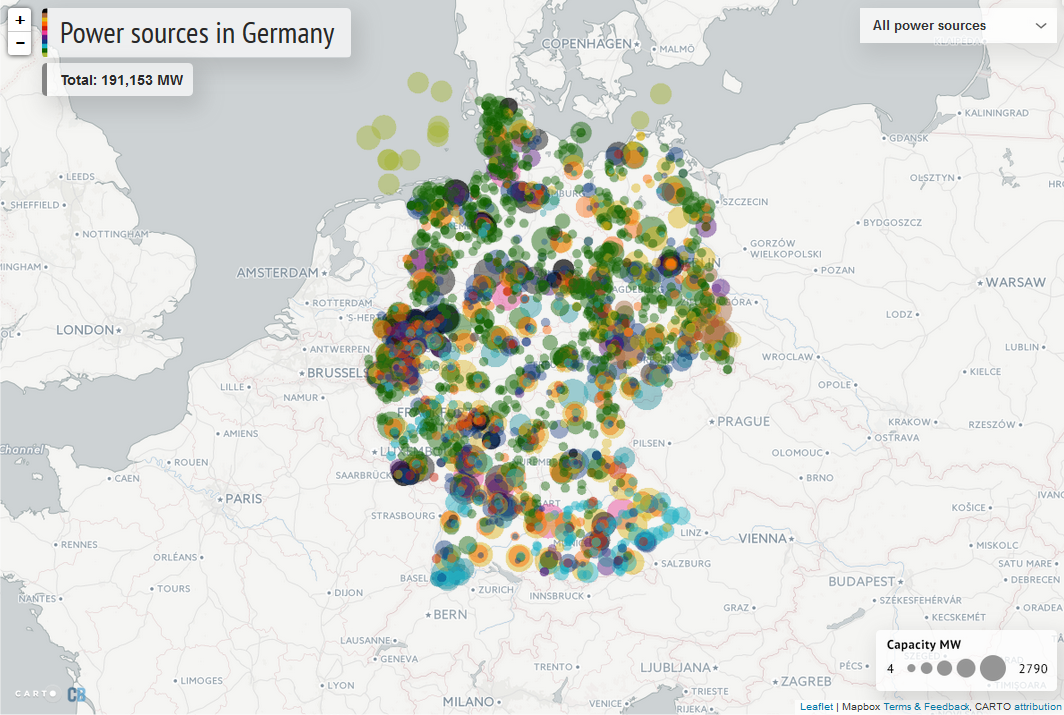
\includegraphics[width=1\textwidth]{mapcb}
    \caption{Interactive map showing the electricity production of Germany}
    \label{fig:mapcb}
  \end{center}
\end{figure}

Another interesting approach to the interactive map was published on July 2015 in the Washington Post \cite{wp2015} under the article of "how United states generate its electricity". This map provides information available power sources and its capacity in MW per US state. Like the previous example, circular area marker is also used here to locate power plants. Unfortunately, its not possible to know the capacity of each source individually. A Choropleth map is used to render different states inside the USA. The user can get information about the total power generated in a state by hovering over any state inside the map. The details of Choropleth map is discussed later in this section. A label is bound to each state which shows the total power generated by each source category and the area of the state is filled with darker color according to the principle of choropleth map. Unlike the previous example, no additional control layers are provided along with the map which makes this less interactive. However, meaningful and self explanatory glyph are used to define each power plants. The color of the logo of a power plant and color of the circular marker of the same power plant is the same. This scheme made easier to focus on each power plant category from a large dense area of the map..

\begin{figure}
  \begin{center}
    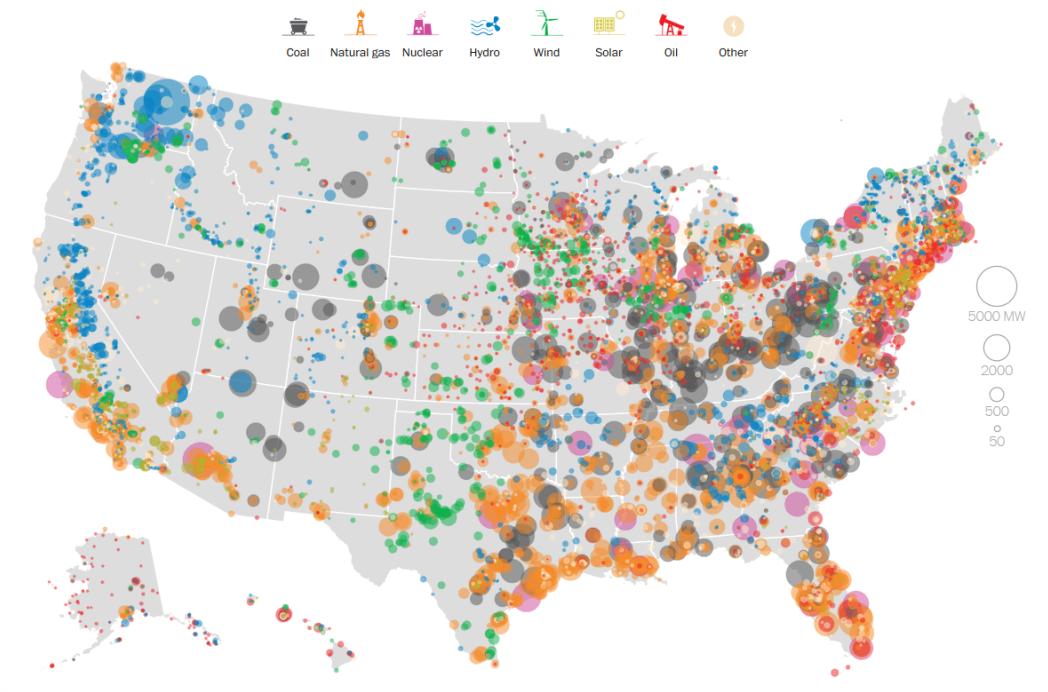
\includegraphics[width=1\textwidth]{mapusa}
    \caption{Interactive map showing how the United States generates its electricity}
    \label{fig:mapusa}
  \end{center}
\end{figure}

Choropleth map, Propotional Symbol map, Pinpoint maps, Connection maps, Isopleth maps are common types. In our case, particularly Pinpoint map and Choropleth are focused for locating the power plants and visualize their density inside Germany. In general, Choropleth Map displays geographical area surrounded by the border or area is colored or shaded in relation to a data variable. This mapping techniques provide a way to visualize density/value over an area. A color progression scale is used to represent the value in each area. On the other hand, pinpoint mapping is used to visualize the exact location of things. Currently, this mapping technique has become more popular. For example, Google Maps show the exact locations of points of interest. Companies from different sectors and service providers are creating their own applications using Google Maps or OSM to provide and share locations of different places such as banks, ATM machines, restaurants, hospitals, shopping malls, roads, rail ways, and shortest paths. We have used this mapping technique to visualize the exact geographical location of the power plants in Germany.

\subsection{Visualization Techniques}

\subsection*{Glyph-Based Visualization}

In different approach for locating renewable and non-renewable power plants and their production 
different countries have adapted different approaches. A common technique that has been observed from research, such as \cite{cbg2016} and \cite{wp2015}, is a circular area on the map. Circular area is the most used marker on the map. Basically, the center of the circle is locating the position and its area is describing the electricity production capacity of that corresponding power plant. These circular areas are filled with colors to categorize the power plants. Circles filled with different colors are easy to identify without deep investigation. To visualize the capacity along with the location of the power plant an ordinal data type is used to compare the size of a circle which is relative to a certain amount of Gigawatts or Megawatts. Mostly a legend is added to the map which provides useful meaning about the circles and helps the user to perceive useful information from the map. On the other hand symbols or glyph are used to represent the object which is the most fundamental way to show the position of power plants on the map. Markers with different colors are also used for easier navigation. Essentially markers can be used to represent anything that has a global position in latitude and longitude coordinates. Every interactive map generation tool provides default markers, which are familiar to most users. However, developers are able to change the markers or add own meaningful marker images. Along with the marker additional label or snippet added to provide more information or description about the marker. This title or snippet is displayed in an info window, a bubble appears over the marker when the user clicks or hovers over the marker.

CarbonBrief \cite{cbg2016} and the Washington Post \cite{gportal2016} have introduced two interactive maps. They provide information on how Germany generates its electricity. Both maps have used a colorful circular marker to locate the position of the plant inside Germany as well as the area of the circle representing the capacity. An internal drop-down navigation menu is added to the map of \cite{cbg2016} where the user can filter the plants by selecting different sources from the menu. On the other hand, \cite{gportal2016} is showing 380kV and 220kV power lines inside Germany along with the circular marker locating the plants and their generation. But there are no menu selection mechanism or filters for showing different power plants on the map. The available interaction techniques might be difficult for the users who are not expert enough using this type of interactive visualization tools. 

However, those approaches are missing the opportunity to engage user into the map on initial view. Circular markers with different colors might confuse the users to interpret the specific type of power plants. In particular, there is more than one unit of power plants are located in the same area. A plant with smaller generation capacity can be overlapped by a plant with larger capacity because of of its larger circular area. Therefore, pin point marker is used in our visualization framework to locate the power plants on the map. Logo inside the marker is self-explanatory and color of the markers is provided by the data set.
 
\subsection*{Interface and Interaction}

In CarbonBrief \cite{cbg2016} a full width map is used with menu selection mechanism (Figure \ref{fig:mapcbm}). With this menu selection, the user can select different categories of power sources. All this menu are hidden in the drop down section. Users are able to select only one category at a time from the menu. There is no possibility to select multiple categories of sources and render them into the map. This restricts users to view their desired power plants on the map. On the other hand, the Washington Post in \cite{wp2015} has published the map with not much functionality. No additional navigation menu is provided along with the map. To get details, user needs to hover over the map.

\begin{figure}
  \begin{center}
    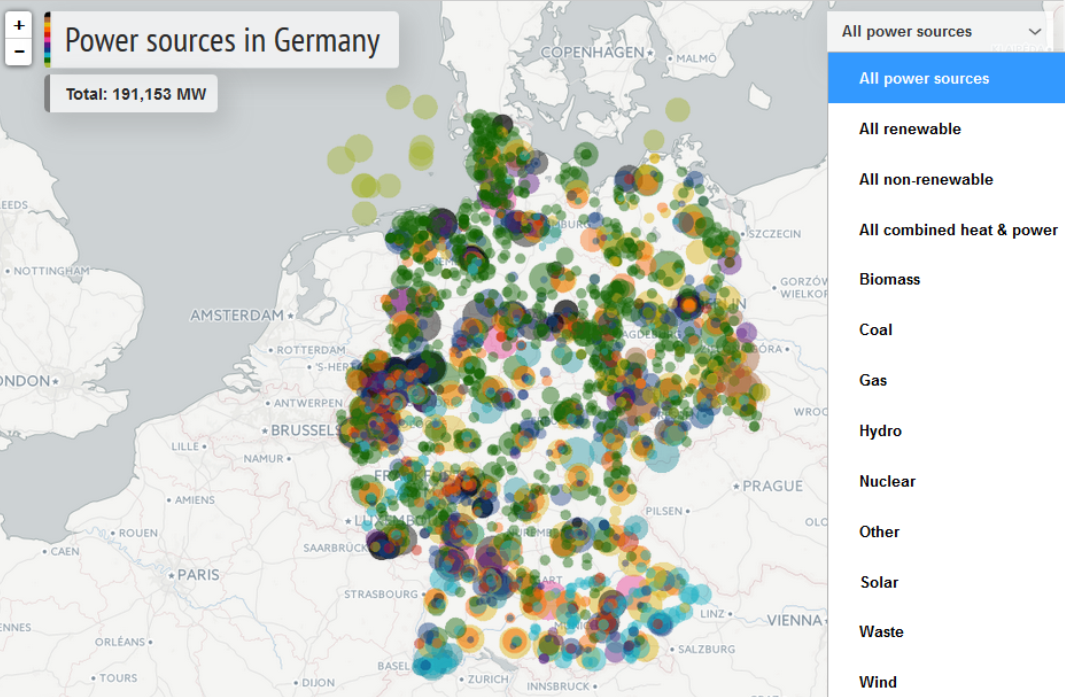
\includegraphics[width=1\textwidth]{mapcbddm}
    \caption{Interactive map : Menu selection mechanism}
    \label{fig:mapcbm}
  \end{center}
\end{figure}

In Geoportal \cite{gportal2016} also published a web based interactive map and providing information with a large and complex interface. Their interactive map has multiple functionality but still, lacks some important features.  For example, they are visualizing the power plants, which has the capacity above 100MW or equal as we are doing with our visualization framework. But there is no scope of power plant selection mechanism (Figure \ref{fig:mapgeo}).   
A descriptive but rather complex legend is added on the map. The user might find it difficult and it would take more time to explore the desired output out of this information visualization technique.

\begin{figure} [H]
  \begin{center}
    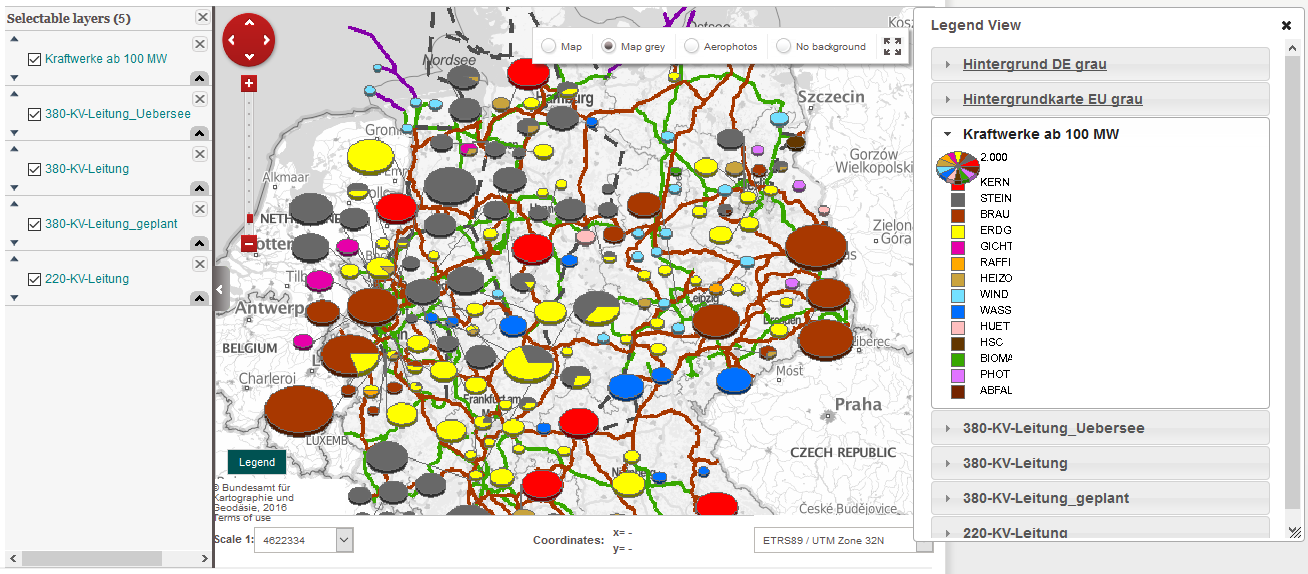
\includegraphics[width=1\textwidth]{geomapcl}
    \caption{Interactive map with Selectable layers and Legend.}
    \label{fig:mapgeo}
  \end{center}
\end{figure}

All these approaches and visualization techniques indeed enable users to extract the desired information from the map. However, in our visualization tool, we tried to make a clear, concise and efficient user interface. It might be easier for the user to figure out how our application works. We also tried to use familiar and consistent approaches to make the interface intuitive and given some more functionality to the users which are somehow missing in \cite{cbg2016}, \cite{wp2015} and \cite{gportal2016}. 

\section{Time series visualization}

There are countless visualization techniques that show time series data in the charts. One of the unique time series visualization is ThemeRiver \cite{981848}. This visualization depicts the thematic variations and changes over time within a large collection of data. The changes are shown in the context of a time line. The main focus of this visualization is to allow users to discern patterns which help to understand trends of the data-set. The theme river flow is directed from left to right. The variation of width represents the variation in the degree of representation unit. The horizontal width between two points on the theme river represents time interval and vertical distance or height of the river at any point of time indicates the strength of that point of the corresponding data set. It shows several streams, i.e. variables which changes over time and lays on top of each other as a layer. In visualization methods for time dependent data, Mueller and Schauman in \cite{1261490} have discussed different conventional approaches for visualizing time dependent data. ThemeRiver is one of the most well-known techniques to visualize multivariate data over Time. An intuitive interpretation of temporal changes can be observed by using this technique. In February 2008 New York Times depicting the “Ebb and Flow of Movies: Box Office Receipts Over Past 20 Years” \cite{boxoffice}. It was an interactive ThemeRiver visualization which illustrates the pattern of the amount of money films over a 21 years period make at the box office. This total figure is shown by varying heights and width that reach over time. A color scale is used to reveal the amount of revenue range. The online response to this visualization was drastic and controversial. Marco and Yifan also mention in \cite{CGF12910} about this New York Times(NYT) publication. Later Byron and Wattenberg \cite{Byron2008} outlined three issues which affected the aesthetics of the graph, e.g, the ordering different layers, the shape of the lowest curve, which suppose to be the baseline and the labels of the layers. ThemeRiver fits in a general mathematical framework. A standard way to visualize time series data is to plot them on a Cartesian graph, which has time on the x-axis and the numeric values on the y-axis. A flat baseline allows the user to easily read the total diagram. 

Later on, this flat baseline strategy has become very popular to visualize power production from renewable and non-renewable energy sources over time this visualization technology has been widely used. In another article of CarbonBrief \cite{cbuk2016}, ThemeRiver visualization technique (see Figure \ref{fig:ukecg}) is used to illustrate how UK is generating electricity over the last 50 years. Around 30\% of the UK electricity came from coal, which is clearly visibile from the illustration. On the other hand, US energy information administration in their Annual Energy Outlook 2017 \cite{eiagov} this flat base ThemeRiver is used to visualize the data for different aspects. Figure \ref{fig:eiatrgh} illustrates an example of it. 

\begin{figure} [H]
  \begin{center}
    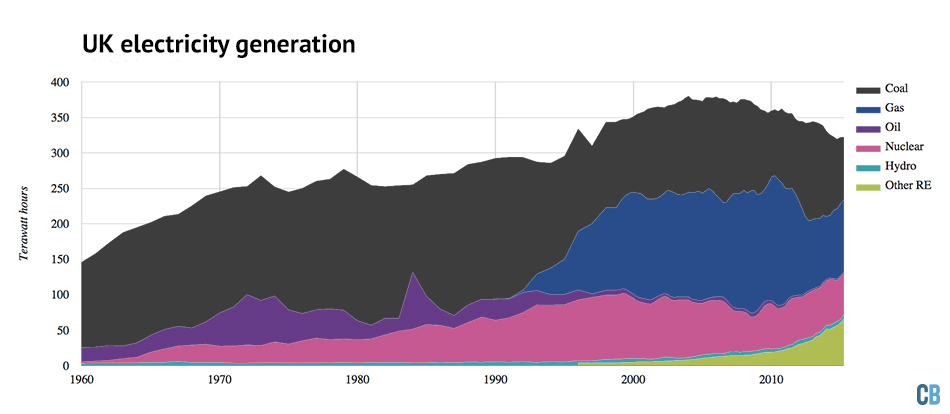
\includegraphics[width=1\textwidth]{UK-electricity-generation}
    \caption{UK electricity generation by fuel type. Source:\cite{cbuk2016}}
    \label{fig:ukecg}
  \end{center}
\end{figure}

\begin{figure} [H]
  \begin{center}
    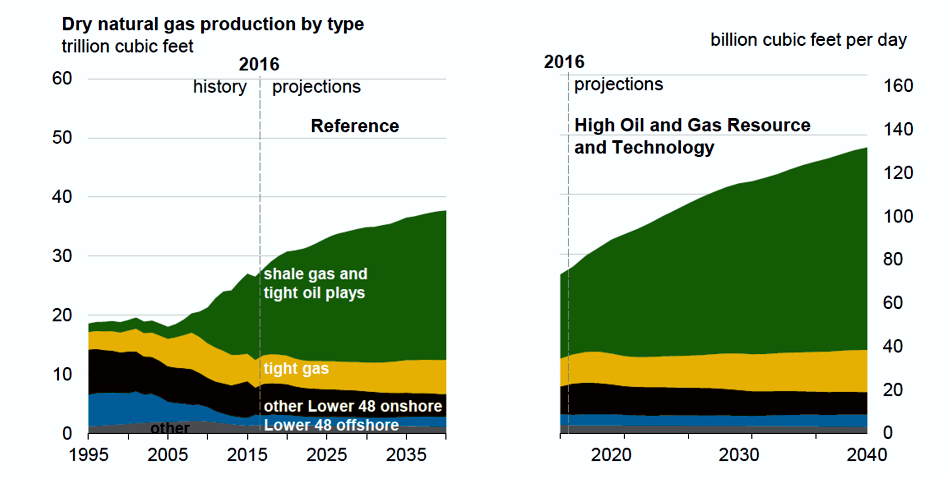
\includegraphics[width=1\textwidth]{eiatrg}
    \caption{U.S Dry natural gas production by type. Source:\cite{eiagov}}
    \label{fig:eiatrgh}
  \end{center}
\end{figure}




\chapter{Background of This Project}
\label{chap:background}

\section{Concept}

The main objective of this project was to make an interactive map with OpenStreetMap to visualize the location of the conventional and renewable power plants. In addition providing the type, production, status and other additional information, which might be interesting for the users. A convenient navigation menu needs to be added to manipulate the data set. Markers dedicated for each power plant would be intuitive. Information for power plants such as the name of the plants, start of operation, fuel type, installed power, grid operator should be displayed in a window or tooltip. Additionally, the high voltage line should be displayed on the map. In our case, three voltages (110kV, 220kV, and 380kV) power lines are displayed in three different unique colors. All these items need to be included in the selection mechanism. The user can select or deselect multiple power plants as well as the power lines according to their interest. As mentioned, information can be extracted from the map with just a few clicks of the mouse. Finally, a tight linking between the 2D graphical map and the temporal plots on \textit{www.energy-charts.de} must be established. This will help the user to see the hourly production for each power plant of different sources. At the end, this interactive map needs to be merged with the \textit{www.energy-charts.de}

Therefore, the creation of this web application was divided into some smaller parts. First, selection of geographical information visualization tool that supports the web environment. Formulation of data in a structured way that supports the visualization tool and web environment, in our case it is JSON. Second, filtering and categorizing the different power plants and power lines from the available data sources. Create a selection mechanism for each category. Third, to map each power plant and power line according to the category and select unique colors for them. Finally, render everything on the map.   
\clearpage  

\section{Tools}

Our online visualization tool is based on JavaScript. For visualizing geographical data Leaflet.js\footnote{Official Leaflet.js Website, \url{http://leafletjs.com/} (last accessed on \today)} version 0.7.7 framework is used. Some additional plugins are used to enhance the performance of the Leaflet map. They are available on the Leaflet website. All the plugins that have been used in the framework will be discussed in Section \ref{olandp}. JSON Data files of power plants are stored on the FTP server.

%Based on the backend the frontend/UI was entirely build %in HTML, CSS, JavaScript. Bootstrap\footnote{Official %Bootstrap.js Website, \url{http://getbootstrap.com/}   %(last accessed on \today)} design system is used for %responsive design. Additionally, a variety of %JavaScript libraries like jQuery\footnote{Official %jQuery.js Website, \url{https://jquery.com/} (last %accessed on \today)} and underscore\footnote{Official %UNDERSCORE.js Website, \url{http://underscorejs.org/}  %(last accessed on \today)} is used to eliminate the need %to reprogram basic functionality.

\section{Leaflet}

Leaflet is an open source JavaScript library for building interactive maps. It is relatively new as it was first released in 2011. It is popular for its flexibility and is used by renowned websites, like Pinterest, Flickr, The Washington Post and Foursquare. It has all features developers need to make an interactive map. It can handle various basic tasks mouse interaction and different map layers can be used. It is easy to extend with a variety of plugins which are available on its web page and plenty of opportunities to extend the basic functionality. It works efficiently across all the browsers as well as mobile platforms.

The map is rendered using tiled layers. Its basic display is implemented by one default basemap. Its build in capabilities enables creating thematic map layers for JSON and GeoJSON data. It also has the ability to draw points, circles, polylines, polygons, custom markers and styling these features dynamically. Among these features, custom markers are used for locating power plants and polylines are used for rendering the power plants on the map. Leaflet also supports Web Map Service(WMS), Vector layers and Tile layers. Power lines on the map are rendered as a vector layers in our framework. Additionally, different tile layers are available along with OpenStreetMap in our framework like streetview, grayscale and, outdoor. Leaflet has a controller that allows the users to see different tile layers as a base layer of the map. It also provides the functionality to add popups to the markers, overlay lines, and shapes. It is extremely light weight and there are no dependencies for this open source library. 

The purpose of using this library is because it is widely used and open source. It supports desktop as well as modern mobile devices. As a whole it is smaller in size, and it takes advantage of the new features of JavaScript and HTML. It is very easy to use and its API is easy to understand for performing common mapping tasks like changing base map, zooming, panning. Leaflet also provides a nice documentation which makes a low barrier to develop new applications.

\section{Other Libraries and Plugins}
\label{olandp}

The significant strength that made leaflet much more powerful is its ability to extend its classes and functionality with third party plugins. There is a large community behind leaflet. At the time of writing, there are more than 100 plugins available on the official website of Leaflet. A couple of plugins are also used in this tool which has a great impact on the performance. The plugins used for our visualization tool are mentioned below.

Plugins for Leaflet framework:
\begin{itemize}
  \item \textbf{Leaflet Marker Cluster}
  \item \textbf{Leaflet Label}
\end{itemize}
External plugins:
\begin{itemize}
  \item \textbf{jQuery.js}\footnote{Official jQuery.js Website, \url{https://jquery.com/} (last accessed on \today)}
  \item \textbf{Bootstrap}\footnote{Official Bootstrap.js Website, \url{http://getbootstrap.com/}   (last accessed on \today)}
  \item \textbf{Underscore.js}\footnote{Official UNDERSCORE.js Website, \url{http://underscorejs.org/}  (last accessed on \today)}
\end{itemize}

\section*{Leaflet Marker Cluster}
\label{sec:clusterr}

A very useful plugins for Leaflet is Leaflet.MarkerCluster. It helps to cluster a large number of markers on a map by providing an animated marker. Its clustering functionality for leaflet has a great impact on the performance of interactive map. It takes less processing time to load the data set and finally it help to make the map look cleaner. The plugin is available for download from the \textbf{Leaflet.markercluster}\footnote{Github Leaflet.markercluster Website, \url{https://github.com/Leaflet/Leaflet.markercluster} (last accessed on \today)} github page. Its CDN link is also provided, which can be used right after the declaration of Leaflet files in the header of the HTML. By default the plugin is providing some nice functionality such as \textbf{showCoverageOnHover}: helps to show the boundary that is been covered by the marker, \textbf{zoomToBoundsOnClick}: when a cluster is clicked it zooms to its bounds.

\begin{figure}[H]
  \begin{center}
\subfloat[All power plants markers of Germany\label{marker}]
  {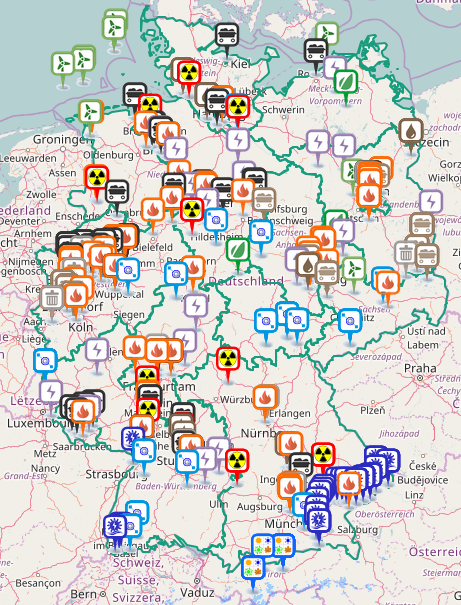
\includegraphics[width=.45\linewidth]{markers_new}}\hfill
\subfloat[Marker Cluster layer on Germany\label{markercluster}]
  {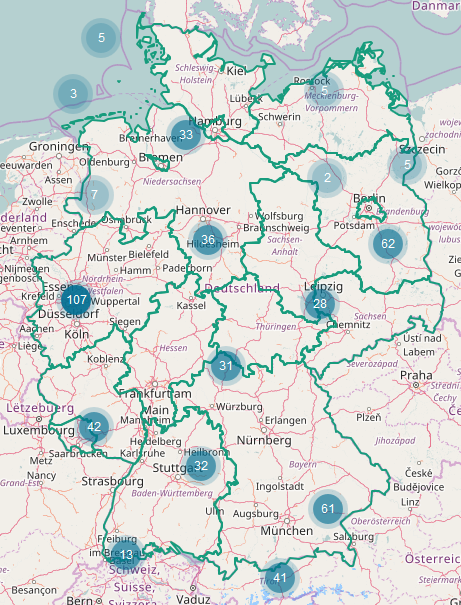
\includegraphics[width=.45\linewidth]{marker_cluster}}
\hfill
\caption{Impact of using marker cluster plugin}
\end{center}
\end{figure}

Figure \ref{marker} shows all the power plants with pinpoint marker inside Germany and Figure \ref{markercluster} shows the impact of using the marker cluster plugin. Clustered animated markers can be customized. Most importantly, it helps to visualize if there are more than one marker rendered in the same geographical location on the map. A cool built in feature spiderfies the child markers of that cluster. Figure \ref{fig:spiderfies} shows that there are in total 13 power plants located in the same area. Hence, to reduce complexity they are registered on a unique latitude and longitude.

\section*{Leaflet Label}

Leaflet label is a plugin for adding labels to markers \& different shapes such as paths, polygons, and circles on leaflet powered maps. \textbf{Leaflet.Label}\footnote{Github Leaflet.markercluster Website, \url{https://github.com/Leaflet/Leaflet.label/tree/0.2.1
} (last accessed on {\today})} development versions are available on GitHub . There is a default style for the label as you can see in the Figure \ref{fig:spiderfies} that power plants are located in Nordrhein-Westfalen. When the user hovers the cursor on the displayed objects of the map, this label appears with the data underlying for that particular object.

\begin{figure}[H]
  \begin{center}
\subfloat[Spiderfy view of multiple power plants located in the same location.
\label{fig:spiderfies}]
  {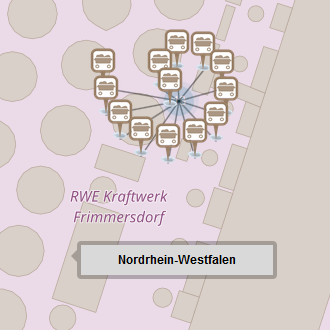
\includegraphics[width=.45\linewidth]{spider_new}}\hfill
\subfloat[Label of a Gas Power Plant\label{popupgas}]
  {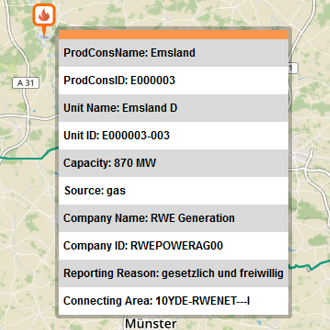
\includegraphics[width=.45\linewidth]{popupgas}}
\hfill
\caption{Impact of using marker cluster and Leaflet label plugin}
\end{center}
\end{figure}

\section*{jQuery}

jQuery is the most popular JavaScript library. Its features are rich. Its syntax is designed to make it easy for HTML document manipulation, handling events, animations, and developing Ajax applications. This free and open-source software enables developers for creating plugins on top of any JavaScript library. In our framework, jQuery is used for DOM element selection and manipulation and for handling events. For example, jQuery is used for the navigation menu in our framework. Our navigation menu is equipped with check-boxes and a drop-down menu. Effect of toggling check-boxes, effect of selecting drop-down menu options, and handling these events on different zoom level are all handled by jQuery. Other applications of jQuery will be discussed in details in Chapter \ref{chap:softwareSystem}  

\section*{Bootstrap}

Bootstrap is well known and free open-source framework. Its popular as front-end framework for designing websites. It is based on HTML \& CSS design with JavaScript extensions. It is dependent of jQuery It provides a responsive structure to the website and compatible with almost all the latest versions of browsers. In our framework, we have used bootstrap to make our website responsive. In particular, it is incorporated for designing the navigation menu of our map.
Bootstrap buttons, check boxes and drop-down navigation menus styling provides a great performance on the websites. These components are interactive and made with JavaScript plugins which are bundled in the Bootstrap package. Furthermore, one of the main reasons to use this plugin is, it offers a good documentation for almost every element what a typical web application requires. So its easy to customize and understandable by any web developer. For creating a nice user friendly interface for web applications with less effort, Bootstrap is a great solution.


\section{Working Environments}

Before developing the online visualization tool of German power plants Fraunhofer Institute for Solar Energy System (ISE) was providing interactive charts on electricity production, electricity stock market prices and import/export of electricity at the website Energy-Charts\footnote{Energy-Chart official webpage, \url{http://www.energy-charts.de/} (last accessed on {\today})}. This whole framework is developed based on JavaScript libraries. For visualizing data, bar chart, ThemeRiver, stacked Multi-Bar chart, and Pie chart are used. To make the chart interactive D3.js\footnote{d3.js official website, \url{https://d3js.org/} (last accessed on {\today})} and NVD3.js\footnote{NVD3.js official website, \url{http://nvd3.org/} (last accessed on {\today})} JavaScript libraries are taken into account. Electricity production of power plants, stock market prices, and import/export data are stored in the web server. There is no database for storing all these data. Therefore, the data used for our visualization tool is also stored in the web server. Other required JavaScript libraries, plugins, dependencies are stored in the webserver of Energy-Charts.

%[language=json,firstnumber=1]
\begin{Listing}[H]
\begin{lstlisting}
var Power_Plants = [
  { 
    "ProdConsName" : "Frimmersdorf",
    "ProdConsID" : "E000005",
    "UnitName" : "Frimmersdorf P",
    "UnitID" : "E000005-012",
    "Source" : "lignite",
    "color" : "rgb(150,125,100)" ,
    "Capacity" : 289,
    "CompanyName" : "RWE Generation",
    "CompanyID" : "RWEPOWERAG00",
    "ReportingAvailableCapacity" : "True",
    "WGS84Latitude" : 51.05629,
    "WGS84Longitude" : 6.57703,
    "Country" : "DE",
    "ReportingReason" : "gesetzlich und freiwillig",
    "ConnectingArea" : "10YDE-RWENET---I",
    "TSO" : "Amprion GmbH",
    "Commercialisation" : 1,
    "StartDate" : "2009-10-26T00:00:00+01:00",
    "EndDate" : "2017-09-30T00:00:00+02:00"
  },
  {....},
  {....}
]
\end{lstlisting}
\caption{An example of JSON-object for Brown Coal(lignite) power plant}
\label{lst:pp-json}
\end{Listing}

\section{File Format}

All the data sources that have been used for power plant visualization and their production in the enrgy charts are in the JSON\footnote{JSON official website, \url{https://json.org/} (last accessed on {\today})}(JavaScript Object Notation) format. This is data format is language-independent and use the extension .json. The MasterData power file is received in CSV (Comma-seperated values) format which is downloaded from the EEX\footnote{European Energy Exchange, \url{https://www.eex.com} (last accessed on {\today})} server. Fraunhofer ISE is authorized to download the files from the FTP server in csv format and later it is converted into JSON data. List \ref{lst:pp-json} shows an example how power plant files are structured in JSON. As we are using JavaScript libraries like Leaflet and NVD3, both support JSON data as input. It is easier to extract information from a large file if data and features are organized in such structured way. 

%[language=json,firstnumber=1]
\begin{Listing}[H]
\begin{lstlisting}
var _110KV_layer = [
    {
      "type": "Feature",
      "id": "way/18957128",
      "properties": {
        "@id": "way/18957128",
        "cables": "3",
        "frequency": "50",
        "power": "line",
        "voltage": "110000"
      },
      "geometry": {
        "type": "LineString",
        "coordinates": [
          [
            6.4336833,
            51.1353571
          ],
          [
            6.4337791,
            51.1353946
          ],
          [
            6.4345818,
            51.1357085
          ]
        ]
      }
    }
   ]
\end{lstlisting}
\caption{An example GeoJSON-object for 110kV power line inside Germany}
\label{lst:pl-json}
\end{Listing}

Another format that has been used for rendering power lines of Germany on the map is GeoJSON\footnote{GeoJSON official website, \url{https://geojson.org/} (last accessed on {\today})}. It is a popular data format among GIS (Geographic Information System) technology and services. Leaflet is very good at handling this GeoJSON format. Power lines inside Germany are created from GeoJSON objects. According to \cite{geojson16}, GeoJSON object is a format for encoding a variety of geographic data structures in the form of geometry and collection of features. GeoJSON supports points, LineString, Polygon, Multipoint, MultiLineString, Multipolygon. Features in GeoJSON contain a geometry object and additional properties and a feature collection represents a list of features. In the list \ref{lst:pl-json}, an example of GeoJSON feature is shown for 110kV power line. These GeoJSON objects are added to the map through creating a GeoJSON layer. The line feature showed in the list \ref{lst:pl-json} belongs to the 110kV layer. Its geometry type is LineString and coordinates are given under the type of geometry. Leaflet creates a GeoJSON layer and adds it to the map.


\subsection{Advantage}

JSON is language independent and programming language model data interchange format \cite{jsonfatfree2006}. This is one of the main reasons for using JSON. It provides a compatibility library for JavaScript, which really supports for reading JSON files using JSON.parse. It is also compatible with browsers and web applications. JSON has a natural way of evolving the data and information. It is very simpler to work with in conjunction with the browser scripting. JSON can be imported into any website, smaller and can represent all Unicode characters. It's also trivial to use it in AJAX applications.
 
On the other hand, GeoJSON is also a data interchange format. It has a standard way of passing information. Leaflet can adopt it well and its performance is very good compare to another available format. It doesn't matter from where it is generated. As long as it is GeoJSON, users can render power lines on the map. It is also easily explorable because it's a regular JavaScript object. This makes the handling easy of large files. Filtering, Styling and then rendering is easy on Leaftlet using this file type.

\subsection{Disadvantage}

JSON is hard to read by a human and it is confusing. Its enormous number of braces, brackets, and commas made it almost unreadable. Therefore, sometimes it is difficult to generate the proper command for parsing the target object from a complex JSON file. It is also not suitable for Big data.  An article \cite{jsontoobig} has described how big is too big for JSON.  Test results show that JSON file larger than 15MB is barely usable in modern browsers. Apparently, in our case, there was no data base available at the time of working. Hence, data are stored on the web server in the format of JSON or GeoJSON. Particularly, GeoJSON data of power lines are larger in size. Therefore, this large data file causes longer execution time for rendering. As a result, the browser crashes sometimes and performance of the map is affected after rendering a lot of polylines on the map. On the other hand, user would never be interested in downloading a large file which consumes so much data, specially on the mobile devices with such limited bandwidth.

\section{Power line(GeoJSON) File Source}
\label{sec:plsource}

In this section, the source of GeoJSON data for power lines and how it is generated using Overpass turbo are discussed.
Data for power lines are extracted from the overpass-turbo\footnote{Overpass turbo API, \url{https://overpass-turbo.eu/} (last accessed on {\today})} API. Overpass API acts like a database of OSM. It also offers search possibilities of power lines. 

\begin{figure}
  \begin{center}
    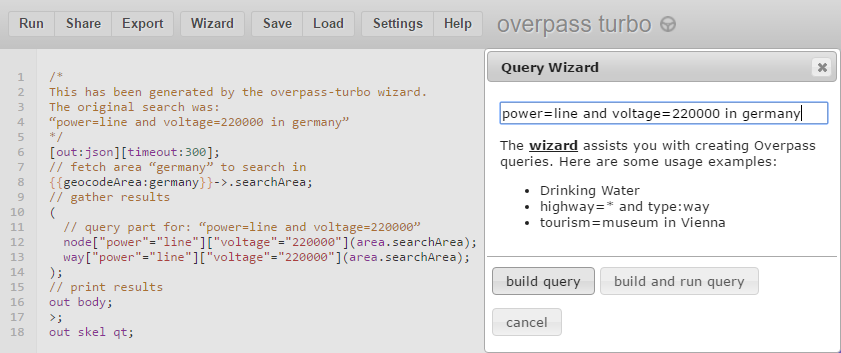
\includegraphics[width=1\textwidth]{wizardfull}
    \caption{Overpass turbo query wizard for generating query}
    \label{fig:wizard}
  \end{center}
\end{figure} 

\begin{figure} [H]
  \begin{center}
    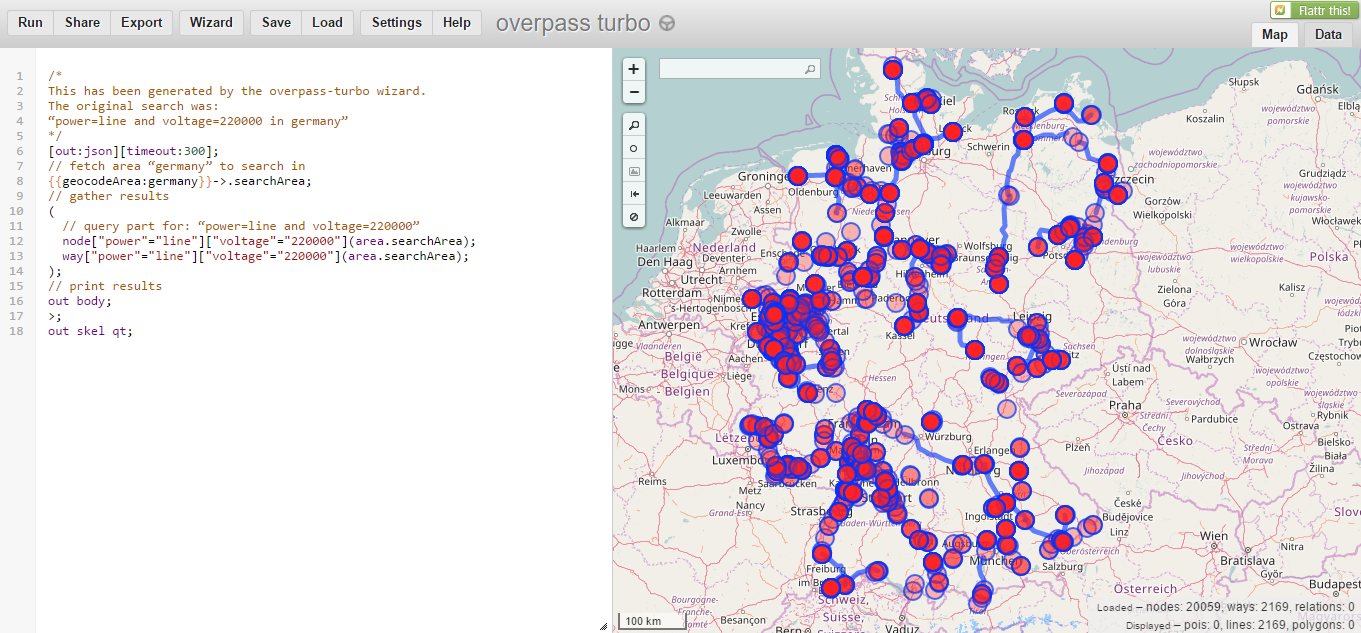
\includegraphics[width=1\textwidth]{optg}
    \caption[Overpass turbo API]{Overpass turbo API query (left) with rendered vector layer of 220kV power line (right) on the OpenStreetMap}
    \label{fig:optg}
  \end{center}
\end{figure} 

For querying power lines a unique tag value must be used. A tag consists of two parts, one is a key and another is value. They are used together separated by an equal. Overpass API uses the tag and serves the part of the OSM map and render it on the map. Therefore, Overpass turbo is used to run the overpass API query. There is a query wizard which assists one generating proper overpass queries. An example is shown in the Figure \ref{fig:wizard}. To get power line for 220kV, one have to fire up the wizard and enter \texttt{power=line} and \texttt{voltage=220000}. Here "power" is a key and "line" is a value of the tag. In addition, fetch area can be selected by simply typing the name of the country inside two curly brackets.
  
After the execution of the query, filtered results are rendered on the OSM. There is an option for exporting rendered data. We exported the data as GeoJSON and used it in our framework. This operation is done twice for exporting the GeoJSON of other two (110kV and 380kV) available power lines. The structure of this GeoJSON is already discussed on the list \ref{lst:pl-json}.

 
\chapter{Software System}
\label{chap:softwareSystem}

The online visualization toolkit is implemented as an additional tool for accessing plant data on Energy-Charts. Energy-Charts is build using JavaScript libraries. Therefore, same, or corresponding technologies were used for our interactive visualization map. 

The vision of this project is to provide an interactive map for users who are interested in Germany’s electricity production.  This visualization tool provides multiple possibilities to explore the Germany’s electricity generation and its distribution. First, users can get an overview of power plants. It shows the location, operating status, and generation capacity of all renewable and conventional power plants in Germany. Second, this interactive map is associated with ThemeRiver or stacked area charts where users can see an hourly production of electricity for each power plant. Finally, the tool also visualizes the power transmission lines (110kV, 220kV, and 380kV) of Germany. Furthermore, users can select multiple power plants and list them in a table chart for comparison. It is also possible to compare those selected units and based on their hourly production with Energy-Charts. 

\section{Requirement Analysis}
\label{sec:reqAn}

As mentioned before, to implement Energy Chart JavaScript library is used. Plant data are stored as JSON files on the server. Hence, for creating an interactive map as an extension to the Energy Chart and to match the functionality with the existing charts, JavaScript mapping library is also used for this project. Our goal was to create an interactive map which is dedicated to the power plants of Germany. Before implementing the tool, the basic must-have components for the map must be specified. Therefore, following things were considered as a list of requirements for the map to enable a quick exchange of information between users and the map.

\section*{System Requirements}
\begin{itemize}
	\item{Need to develop an interactive map with OpenStreetMap open source JavaScript libraries.}
	\item{For having no data base, our tool must be able to access JSON files from the server using AJAX query and deliver it to the map.}
	\item{The interactive map should run on web platform, support web technologies and usable on modern smart devices.}
\end{itemize}

\section*{Interface Requirements}
\begin{itemize}
	\item{To visualize the location of the plants, glyph based visualization technique can be used. A meaningful map marker must be used for each fuel source category. A fixed color code is assigned to each source category.}
	\item{In the case of mouseover or clicking event a marker, window, or tool-tip must appear displaying the basic information of the power plants. Displayed information needs to be extracted from given JSON files.}
	\item{In addition, the high voltage power lines should be displayed on the map for three voltages 110kV, 220kV, and 380kV.}
	\item{To complete the interface, a simple, clean, and effective navigation menu must be designed and should be placed above the map to display or hide different types of power plants and high voltage power lines.}
\end{itemize}

\section*{Functional Requirements}

\begin{itemize}
	\item{Internal communication between the interactive map and Energy-Charts must be established. Thus, the users can query plant data, see their hourly production, and can make a comparison.}
	\item{The map and energy charts have to be linked. Therefore every selection is reflected in both and that people should be able to chose individual power plants.}
	%\item{A way of comparison between power plants must be established.}
	\item{Navigation menu and its utility  should offer adequate possibility to allow user for controlling the view on the map API}
\end{itemize}

Therefore, to achieve and implement the above-mentioned requirements we decided to use a simple lightweight JavaScript mapping library – Leaflet.  Finally, we end up with a fully-clickable interactive map as a composite image consisting of a map, location markers and poly lines. 

In the following, we will give an overview of the architecture and explain the graphical user interface of the visualization tool.

\section{Architecture}
\label{sec:architecture}

The diagram in Figure \ref{fig:architecture} shows the architecture of the complete interactive map and its connection between server-side and client-side. 

Back-end is developed based on JavaScript along with the Leaflet. Additionally, jQuery and underscorejs are used to eliminate the necessity to reprogram the basic operation and functionality. Multimedia contents and JSON files are loaded on the FTP server. 

Initially, leaflet and additional JavaScript code for creating the map API are executed on the page load. By default, JavaScript code makes request to the file server over HTTP and get JSON files as a response. Location of all power plants are preserved in that JSON file. Leaflet parses the JSON file and render the power plants on the map. During this operation program also set the marker properties. Each source category has a unique marker image which are also stored in the server. At the end users get an interactive interface and can see the map on the screen with some colorful markers of power plants locating its location on the map. 

There is an individual script that executes after page load for establishing the connection between front-end and back-end. All the JavaScript events for navigation menu, buttons and map zoom-in/out events are registered there. The large GeoJSON files for high voltage power lines are not initially loaded. User needs to use the navigation menu for sending a new HTTP request to see them on the map. Server identifies the path of the requested file through scripts and returns the GeoJSON file to the client side. Finally leaflet parses the GeoJSON data and render it to the map.


\begin{figure}
  \begin{center}
    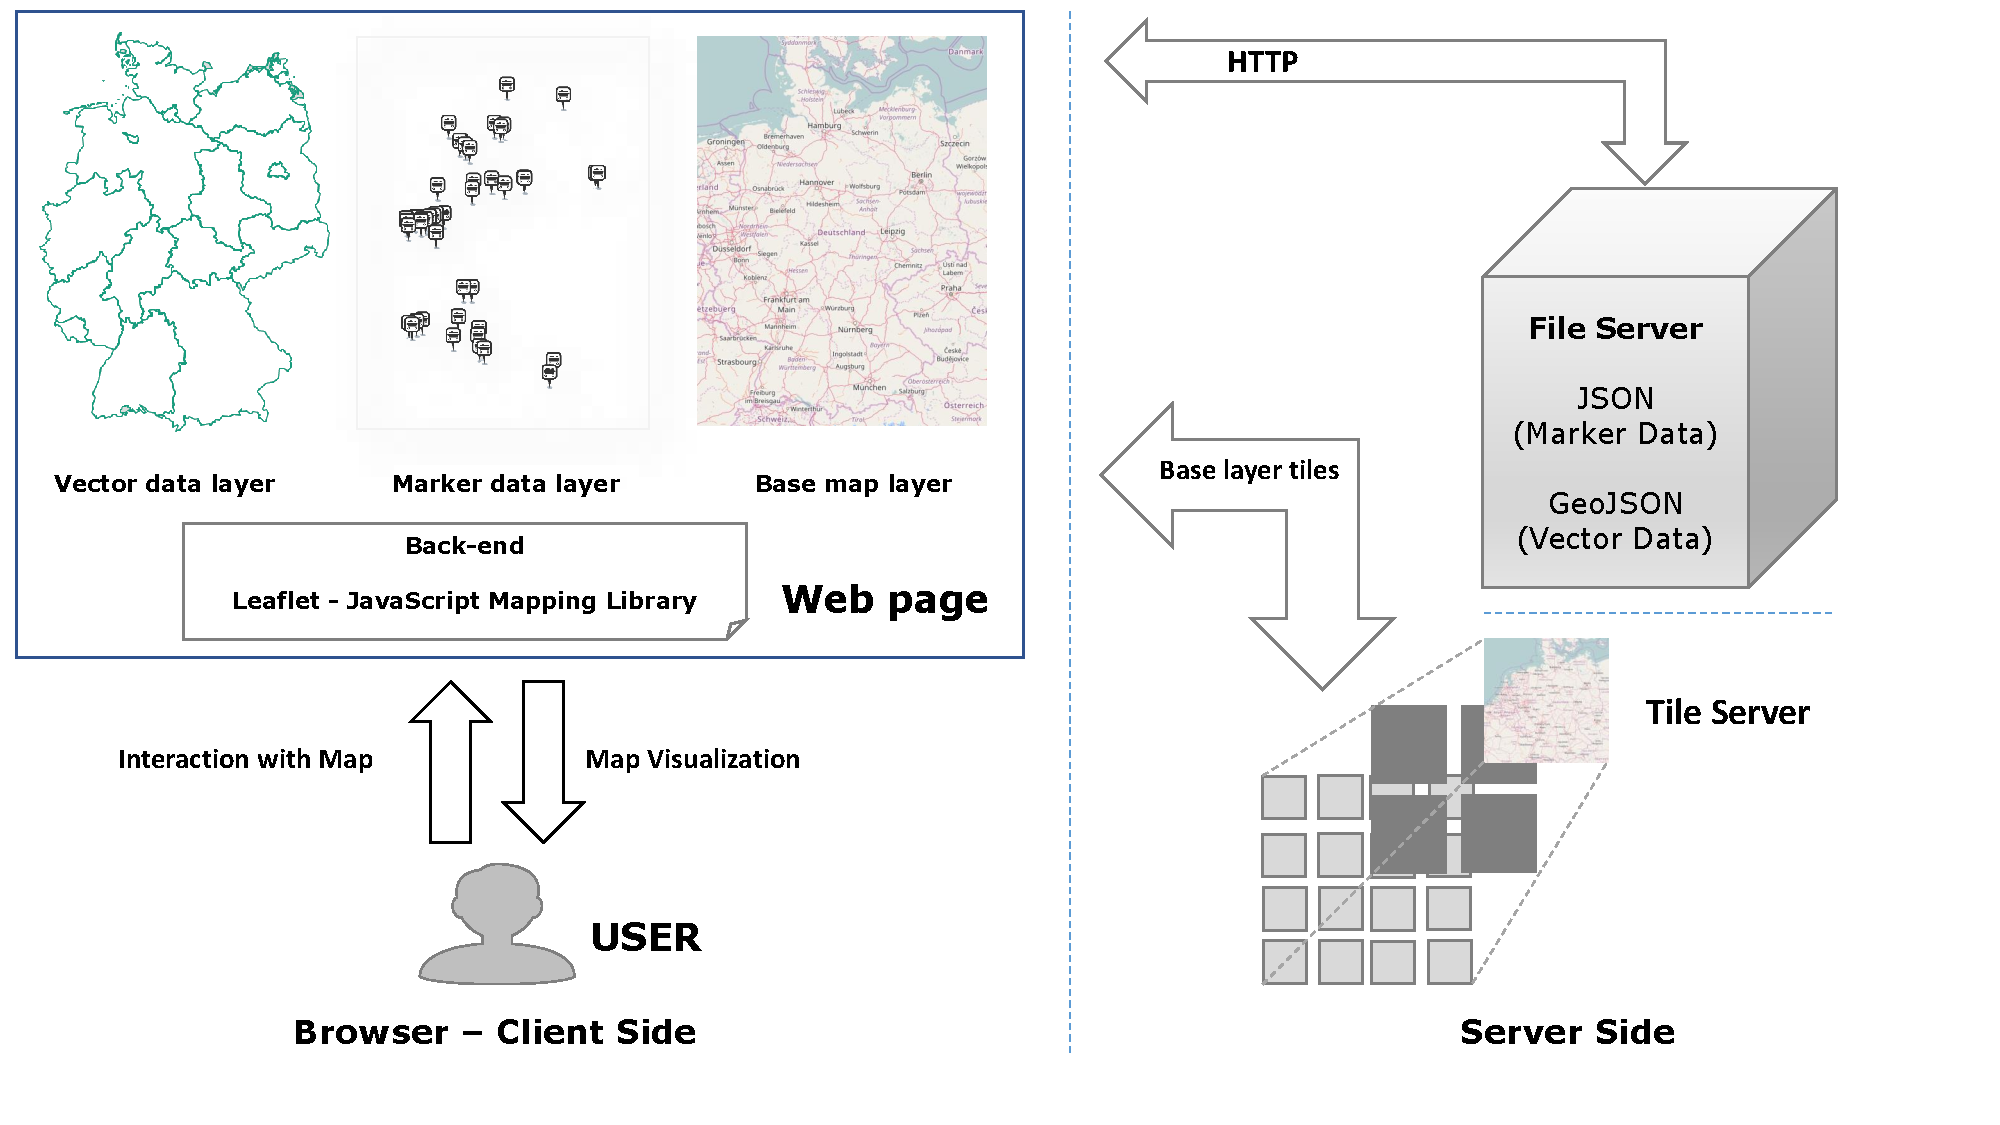
\includegraphics[width=1\textwidth]{architectureNew}
    \caption[The architecture of the visualization tool]{The architecture of the visualization tool - connection between back end and front end}
    \label{fig:architecture}
  \end{center}
\end{figure} 

\section{User Interface}
\label{sec:ui}

Based on the back-end the front-end is entirely developed in HTML, CSS, and JavaScript using the existing template for Energy Charts. Bootstrap design system was chosen for interface(e.g navigation menu, buttons and drop down) design and making the web page responsive. Furthermore, the user interface of interactive map is designed for desktop computers as well as smart mobile devices. In the following, the main structure of the graphical user interface containing the navigation menu, map API as well as the comparison chart will be presented. The main structure is shown in the Figure \ref{fig:structure}. As this interactive map is integrated into the Energy-Charts page, therefore the same template is used for the header section. Our graphical UI starts right after the navigation menu of the Energy-Charts page. Our interactive visualization tool starts with a navigation menu which can also be called as a control layer for the map. Check-boxes are used for the navigation menu area to externally control the map. They are decorated with unique colors. These colors are matched with the colors that have been assigned to each source category in the JSON file.  The map is located under the control layer where markers, power lines, and their basic information are displayed. An area for comparison list is allocated on the web page. Comparison table chart only appears when a user selects a power plant for comparison. Depending on the device, the appearance of the comparison list may change. Hence, our online interactive data mapping tool consists of three main parts: 

\begin{itemize}
	\item{Control Layer: Navigation menu with two subsections}
	\item{Map API: Cluster layer, markers, high voltage power lines, legends and basic information in the pop-up box}
	\item{Comparison List: Comparison table chart for comparing power generation of the power plants that fall under same source category.}
\end{itemize}

\begin{figure}
  \begin{center}
    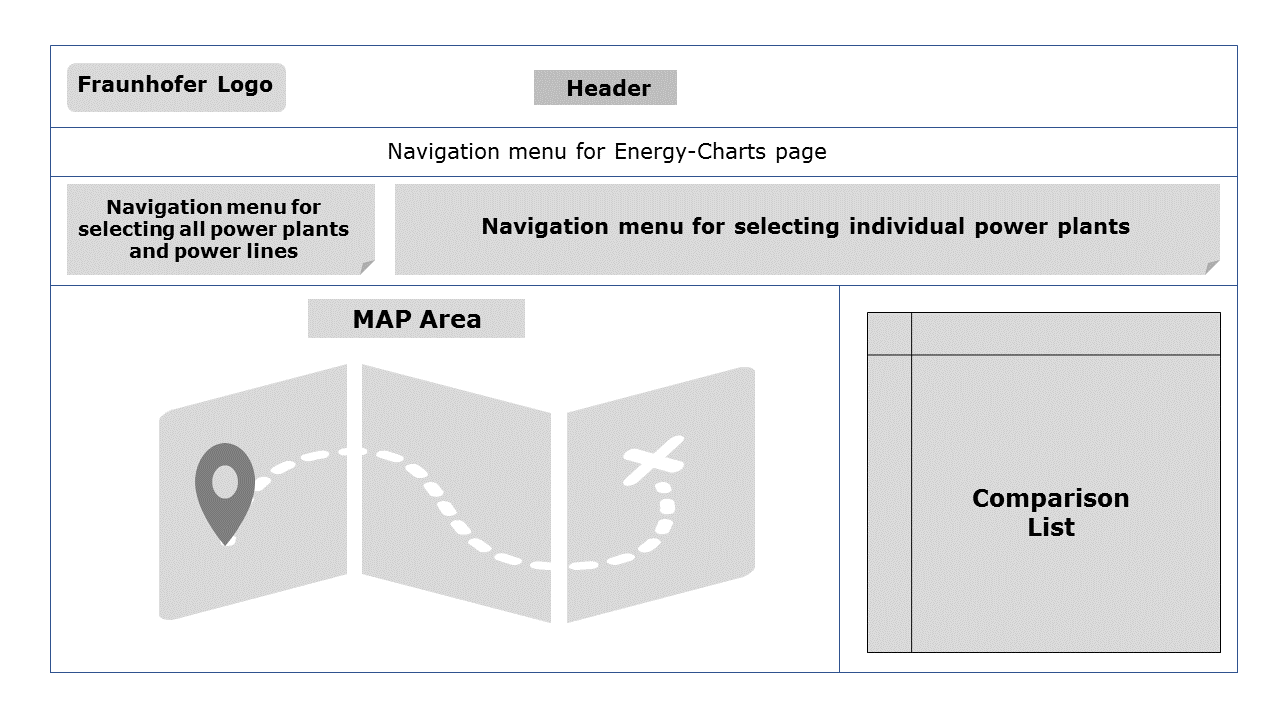
\includegraphics[width=1\textwidth]{structure}
    \caption{The main structure of the visualization page}
    \label{fig:structure}
  \end{center}
\end{figure}

In the following these parts are particularized in details.

\subsection{Control layer}
\label{sssec:controlLayer}

Control layer provides the functionality to manage the displayed content on the map. Check-boxes are used to control the map using external JavaScript events. It is possible to design these boxes in different ways. This circular design is inspired by the legends of energy power chart. For this reason, we designed this external navigation menu for controlling the map. Control layer is divided into two sections (See Figure \ref{fig:menuu}).

\begin{figure} [H]
  \begin{center}
    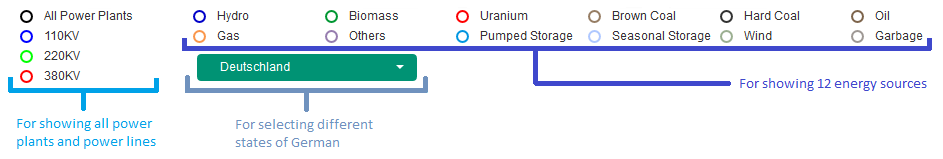
\includegraphics[width=1\textwidth]{menu}
    \caption{Navigation menu}
    \label{fig:menuu}
  \end{center}
\end{figure}


Check-boxes for selecting all power plants at once, and for high voltage power lines are located on the left side of the navigation menu. In the remaining space, check-boxes for selecting individual energy sources category are placed on the right side of the navigation menu. As provided in the JSON data, there are 12 energy source categories are provided in the navigation menu. Check-boxes are decorated with a circle with a border and a label next to the circle. A tool tip appears under it if the user hovers the mouse over the check-box (see Figure \ref{fig:menuTT}. Check-box area includes the circular check-box and its label. 

\begin{figure} [H]
  \begin{center}
    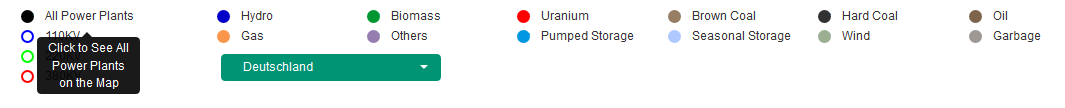
\includegraphics[width=1\textwidth]{menu_tooltip}
    \caption{Tool tip for Check-boxes}
    \label{fig:menuTT}
  \end{center}
\end{figure}

A drop-down selection menu is designed to locate and select 16 different states of Germany on the map. %sIt can be used to select between 16 German states in the form. It contains a header and labels for each state. 


\subsubsection*{Control Layer Properties}

Control layer is an essential part of the interactive map. To perform an action, the user needs to select check-boxes. When the status of the check-box is not selected or unchecked, its appears as an empty white circle with a colored border. On selection, it is filled with its previously assigned border color (see Figure \ref{fig:menufilled}) and reveals the power plant on the map. For example, to show all power plant on the map the user must click on the check-box labeled with “All Power Plants”. This action triggers all 12 check-boxes of power plants and fills the circles with colors (see Figure \ref{fig:menu2}). While continuing this operation if any one of the power plants is unchecked or deselected, then “All Power Plants” is automatically deselected.  On the other hand, if all 12 check-boxes are selected manually, this action also selects the check-box of “All Power Plants”. Therefore, based on selection the content of the map will be updated. Same properties and behaviors are also applicable for individual high voltage power lines. To see the power lines on the map, the user must select the check-boxes assigned for each power line. 

\begin{figure} [H]
  \begin{center}
    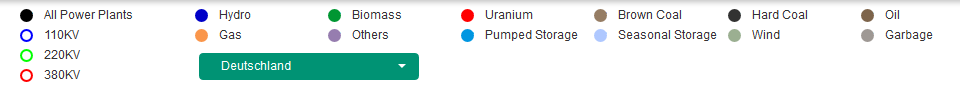
\includegraphics[width=1\textwidth]{menu_filled}
    \caption{Navigation menu with all power plant selected.}
    \label{fig:menufilled}
  \end{center}
\end{figure}

\begin{figure} [H]
  \begin{center}
    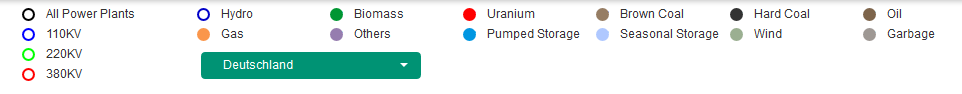
\includegraphics[width=1\textwidth]{menu_one_not_selected}
    \caption{Navigation menu where one energy-source is deselected.}
    \label{fig:menu2}
  \end{center}
\end{figure}

The drop-down selection mechanism for German states is also a part of the control layer. It was added to give users an opportunity to control the map and find different states inside Germany. Users can choose between 16 states from the menu for zooming in and to have the local view of that particular state. This animated zoom-in option uses a feature of Leaflet to get the bounds of the selected state data layer and fits on the map with the maximum possible zoom level. This will help the user to get an idea about the power plant density inside the selected state of Germany. The user needs to select “Deutschland” to restore the global view of the German map. Figure \ref{fig:stateSelection} shows an example of state selection mechanism. On the selection of Baden-Württemberg from the drop-down list, it is highlighted, and map zoomed in to fit it on the map screen.

\begin{figure}
  \begin{center}
    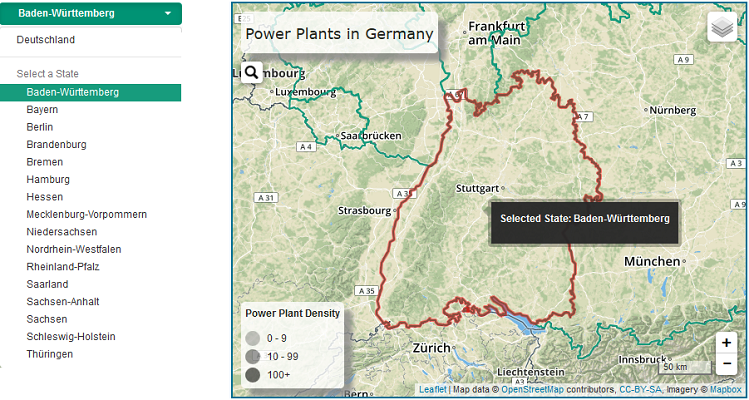
\includegraphics[width=1\textwidth]{state_selection}
    \caption[A German state (Baden-Württemberg) is highlighted]{A German state (Baden-Württemberg) is highlighted, when it is selected from the drop-down navigation menu}
    \label{fig:stateSelection}
  \end{center}
\end{figure}

\begin{figure}
  \begin{center}
    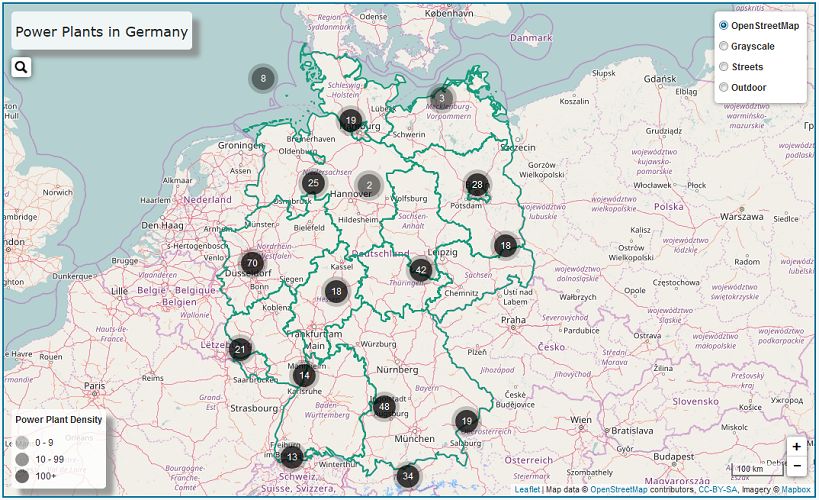
\includegraphics[width=1\textwidth]{map_view}
    \caption[Interactive map area]{Interactive map area equipped with legends on (top-left and bottom-left), initial cluster view, zooming and map scale control (bottom-right), different base map layer controller(top-right)}
    \label{fig:mapView}
  \end{center}
\end{figure}

\subsection{Map API}
\label{sssec:mapArea}

The interactive map appears under the navigation menu on the web page. Our initial view of the map, when the page opens, is illustrated in Figure \ref{fig:mapView}. After initializing the map, the default view of the map is set to Germany with a zoom level 6. Therefore, the entire map of Germany is visible in the map area. The area is equipped with legends, zoom controller, and map scale controller. The custom control layer is collapsed and placed on the top-right corner of the map. Beside these, another information layer is added by default to highlight the border of Germany and its states. This vector data layer is a collection of polygons and stored as GeoJSON on the server. This GeoJSON was extracted from GitHub\footnote{Databundeslander, \url{https://gist.github.com/oscar6echo/4423770} (last accessed on \today)}. In addition, a cluster view of all markers was created using Leaflet.MarkerCluster plugin and was added to the map. This cluster view could help the user to understand the density of power plants of a particular area. The number written inside of a cluster represents the total number of markers contained under this. Cluster layer is filled with black color and its opacity depends on the density of the markers. A custom control legend is added to the bottom-left corner of the map area describing the color scale. When user mouse over a cluster it shows the bound of its markers and if the user clicks on a cluster it zooms to its bounds. As discussed in Chapter~\ref{chap:background} Section~\ref{sec:clusterr}, this plugin is also helpful to find if there are more than one plant located at the same position on the map.

\subsubsection{Functionality}
\label{sssec:functionality}

\begin{figure} [H]
  \begin{center}
    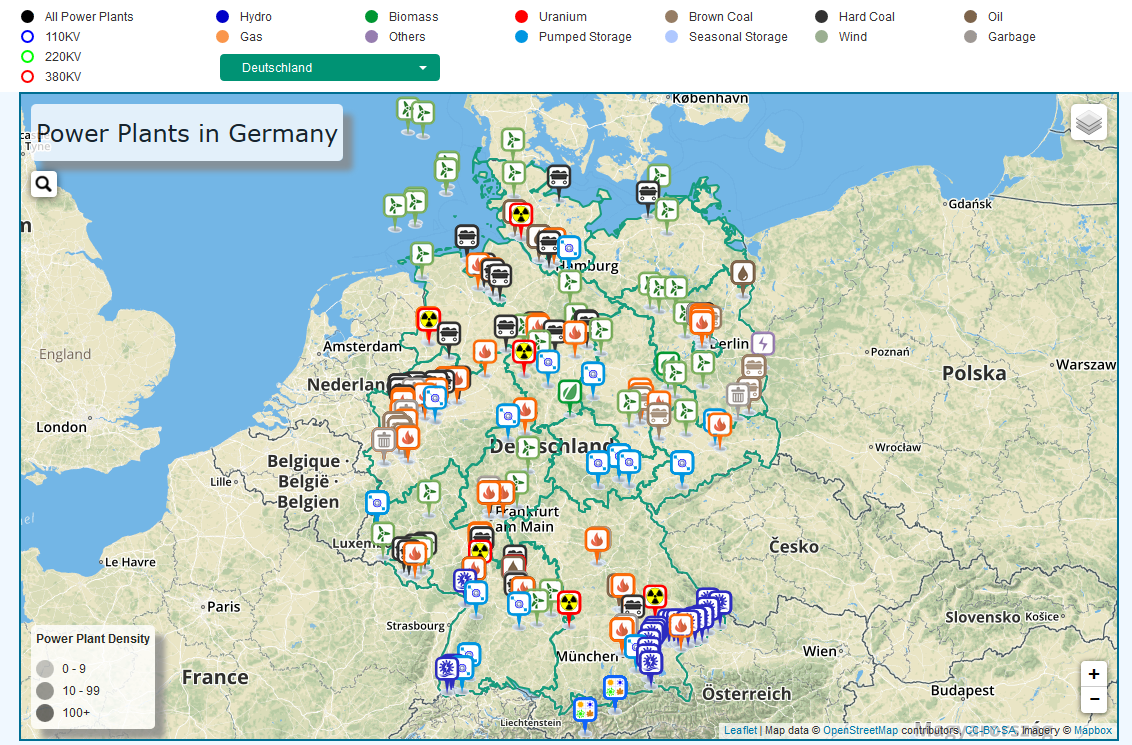
\includegraphics[width=1\textwidth]{marker_ini}
    \caption{Showing the geographical location of all power plants with markers.}
    \label{fig:markerini}
  \end{center}
\end{figure}

In this section, the functional aspects of our visualization tool in the combination with our control layer are discussed.

As discussed in Section \ref{sssec:mapArea}, by default a cluster view of all power plants are rendered on the map. This is added as a layer on the map. Cluster view interprets that there are no check-box selected or no action was performed externally on the map. From this position, users can zoom in by clicking the zoom-in button or even by scrolling the mouse. Markers smoothly split from the cluster on zoom-in and merge to its cluster on zoom-out. If any check-box is selected, this action will remove the cluster layer from the map. In the case of viewing all power plants on the map, the user needs to select “All Power Plant” and as a result, all the markers are visible on the map (see Figure \ref{fig:markerini}). For Each energy source category, a unique color and marker logo are assigned. At the time of reading the JSON data, markers are categorized and stored in groups. Each object of layer group is rendered on the map as a check-box input. For example,  to see all nuclear power plants, the user needs to select the check-box labeled “Uranium”. In that case, only the nuclear marker layer object is added to the map (See Figure \ref{fig:uranium}. Here, jQuery is used for targeting the html DOM (Data Object Model) input check-box object and leaflet functionality is used to add it to the map. 

\begin{figure}
  \begin{center}
    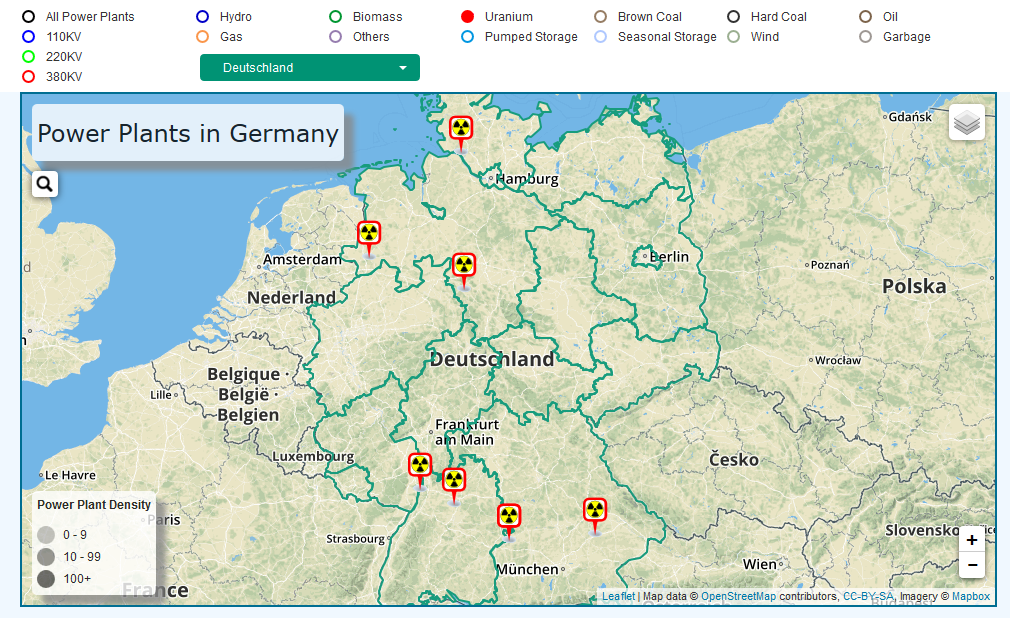
\includegraphics[width=1\textwidth]{uranium_selected}
    \caption{Showing all nuclear power plants.}
    \label{fig:uranium}
  \end{center}
\end{figure}

Along with the geographical location representation, information about each power plants have also been attached to its location marker. Every time a user clicks on a marker a pop-up is attached to it with a specified HTML content and finally, the pop-up appears on the center of the map. We have used a custom design for the pop-up. It is a table with details on the power plant, two buttons, and colored border. Figure \ref{fig:mpp} shows two different pop-up boxes for two different power plant categories. It is clearly visible that they are similar in structure but not in color. The color of the border and the button varies for different categories. This pop-up box is used for displaying the basic information of power plants from the JSON. Basic information includes unit name,unit id, source, capacity, company name, start date and some other additional information. 


\begin{figure}
  \begin{center}
\subfloat[A marker pop-up of Gas power plant\label{fig:gaspp}]
  {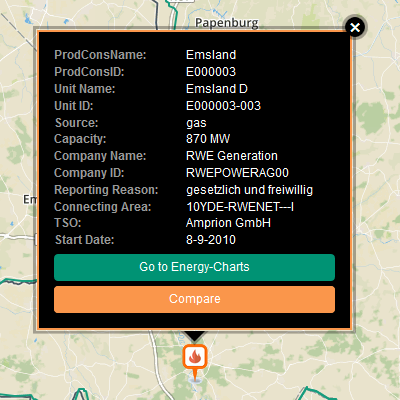
\includegraphics[width=.45\linewidth]{gas_pop}}\hfill
\subfloat[A marker pop-up of Nuclear power plant\label{fig:npp}]
  {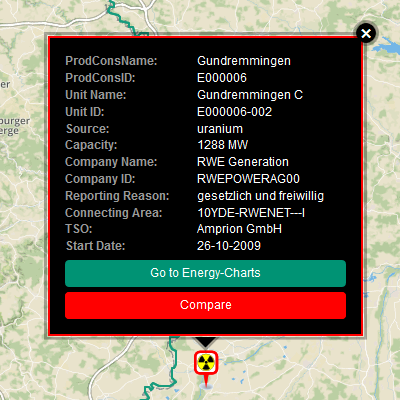
\includegraphics[width=.45\linewidth]{uranium_pop}}
\hfill
\caption{Marker Pop-up box}
\label{fig:mpp}
\end{center}
\end{figure}

\subsubsection{Connectivity between map and energy-charts}
\label{sssec:connectivity}

In this section, the connectivity between interactive map and energy chart is discussed. This was one of the main functional requirements for our interactive map application.

Our goal was to access and view the hourly electricity production data of each power plant from the interactive map. Therefore, an internal connection is established. Users can select power plants and send a query to the energy charts to see their production. If the data of that specific power plant unit is available on the server, then hourly production of that power plant will be illustrated on energy charts. Users are informed over a browser pop-up window on the energy chart page if there is not data available.

The interactive map provides two possibilities to access power plant data on the energy charts. First approach, using the “Go to Energy-Charts” button, which acts as a link (see Figure \ref{fig:buttons}.  Users can send a query by clicking on the “Go to Energy-Charts” button to directly view the time line visualization of electricity production. Each of this button has a unique link for sending queries. These links are dynamically generated while inserting the basic information of power plants in the pop-up box. This link delivers information to the chart. These information are \textit{source} and \textit{ID}. Each power plant has a unique unit id and source category, which are provided inside the power plant JSON data as an object. The hourly production JSON data also have the same object for unit id but its source category is specified inside the file name. Therefore, the value of \textit{source} variable is required to query the desired file and the value of \textit{ID} is required to match the desired power plant data. Hence, only one power plant production data is visible on the hourly production chart and others visibility are hidden. Second approach is using the "Compare" button, which leads to the Comparison List. Comparison list and its application for accessing electricity production data is discussed in the Section \ref{sssec:comparisonList}.

\begin{figure}
\centering
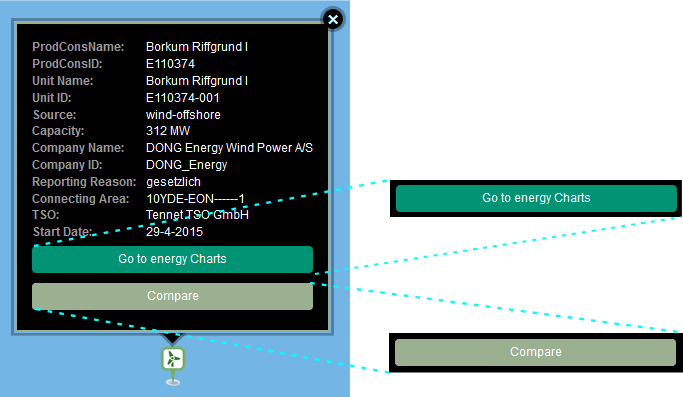
\includegraphics[width=1\textwidth]{buton}
\caption[Buttons inside pop-up box]{\textit{Go to energy charts} button - to see its electricity production on energy chart and \textit{Compare} button - to add this plant to the comparison list}
\label{fig:buttons}
\end{figure}

\subsection{Comparison List}
\label{sssec:comparisonList}

Our interactive map provides an additional feature, where users can compare multiple power plant, and in the end, users can view their hourly electricity generation on the chart. A click on the “Compare” button (see Figure \ref{fig:buttons}) generates a comparison list (see Figure \ref{fig:ctable}) on the interactive map page. The comparison list will appear next to the map (or below, for mobile devices). Users can dynamically add more power plants to the list. Newly added plants are listed as a new entry on the table. If a plant is added to the table then its “Compare” button is disabled and marked as “Selected”. This function prohibits adding the same element several times to the list. The hourly production data of the power plants in the comparison list can also be shown in the Energy Charts by clicking the “Compare on Energy Charts”. This describes the second of approach for accessing hourly electricity generation data. Like “Go to Energy-Charts” button, “Compare on Energy-Charts button also acts as a link. This new button also passes information upon clicking it. Unlike the first approach, this link passes the information from the comparison table. Therefore, more than one power plant data is visible on the charts. Figure \ref{fig:eccharts} shows the hourly production data for the wind-offshore power plants because only those three power plants are listed in the comparison table. This function runs when users click on the "Compare on Energy Charts" button. 

\begin{figure} [H]
\centering
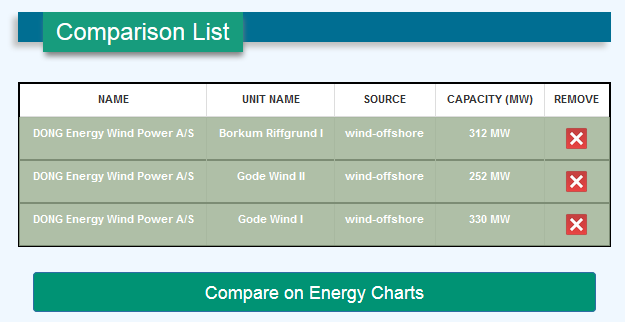
\includegraphics[width=1\textwidth]{comparison_table_wind}
\caption[Wind-offshore(3) power plants are listed on the comparison table]{Wind-offshore(3) power plants are listed on the comparison table. Table also includes a button (\textit{Compare on Energy Charts}) to see their hourly production on energy chart.}
\label{fig:ctable}
\end{figure}

\begin{figure}
\centering
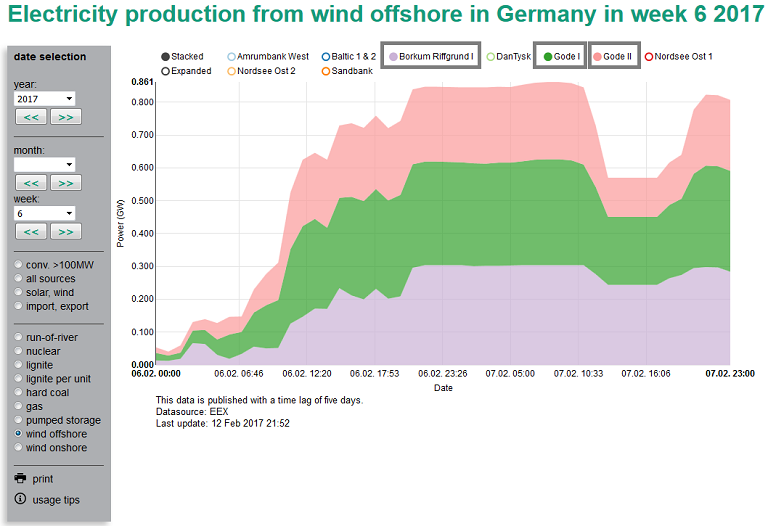
\includegraphics[width=1\textwidth]{ecchart}
\caption[Energy Chart showing the hourly production data]{The chart is created after clicking the "Compare on Energy charts" button in Figure \ref{fig:ctable}. Wind-offshore is selected in the left navigation area (source) and only listed power plants are selected and the rest are deselected.}
\label{fig:eccharts}
\end{figure}

Only power plants from the same source category can be compared on the comparison list. Users can add as many power plants as needed in the comparison list from different source category but this approach disables the functionality to compare them on energy charts page. For example, if users are interested to view the electricity production of Nuclear(Uranium) power plants then users should include only Nuclear power plants to the comparison list and use the "Compare on Energy Charts" to see their production. Currently, the energy charts can only illustrate the hourly data for a single source category. There is a form, inside the gray area with some radio buttons, for controlling the chart and to see the electricity production on the chart for different sources (see Figure \ref{fig:eccharts}). Energy charts provides the unit wise electricity production data for Hydro, Nuclear, Brown Coal (lignite), Hard Coal, Gas, Pumped storage, Oil, Wind-offshore, and Wind-onshore power sources. At present there is no data available for Biomass, Seasonal storage, Garbage, and Others source category. Therefore, it is not possible to see their production and compare them on energy charts.   

\section{Data query process on energy charts}
\label{sec:algorithm}

In the Section \ref{sssec:connectivity}, how the interactive map is connected to the energy charts is already discussed. The algorithm used for solving this functional requirement is separated from that discussion and described here in details. 

As mentioned before there are two different ways to access and view the hourly electricity production data. The basic difference between these two approaches is not much. “Go to Energy Charts” button passes only two variables (\textit{source} and \textit{ID}) over URL and direct to energy chart page. Figure \ref{fig:url} shows how the underlying link of the button is updated dynamically. 

\begin{figure}
\centering
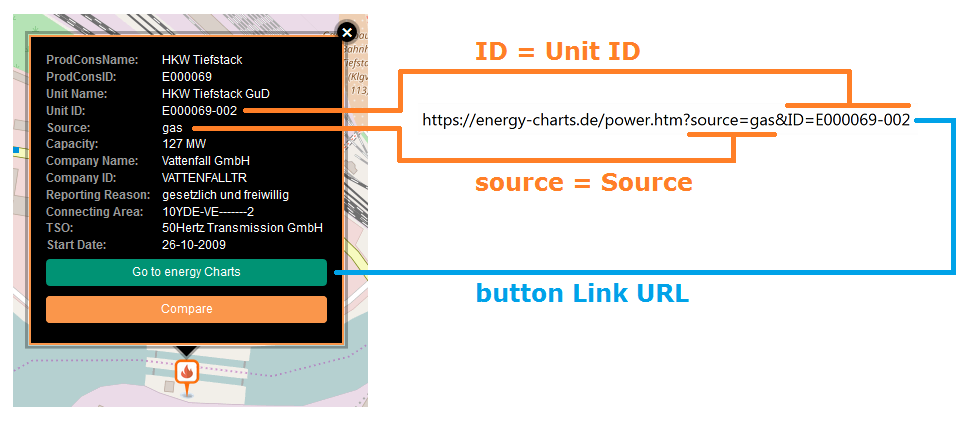
\includegraphics[width=1\textwidth]{url}
\caption{Hyperlink of "Go to Energy Charts"}
\label{fig:url}
\end{figure}

The functionality of "Compare on Energy Charts" button is also discussed before in Section \ref{sssec:connectivity}. The functionality of this button is to pass one or more unit ids over the URL. When a user adds a new power plant to the comparison list, the unit id of that power plant is added inside the \textit{ID} variable. Consequently, the link of the "Compare on Energy Charts" button is updated in the background. Figure \ref{fig:stepsPP} shows different steps of adding more than one power plant in the comparison list and how the link is updated in every step. This approach starts when users want to compare one or more than one power plants. For example, a user wants to compare the capacity and hourly production of three Nuclear power plants. In Step 1, user opened a pop-up window of a Nuclear plant and added this to the comparison list by clicking on the "Compare" button. Step 2 and Step 3 can be done in the similar way. Therefore, two more power plants are added to the comparison table. Thus, in total three unit ids are added to the \textit{ID} and the redirect link for "Compare on Energy Charts" is updated as showed in the Figure \ref{fig:stepsPP}. 

\begin{figure} [H]
\centering
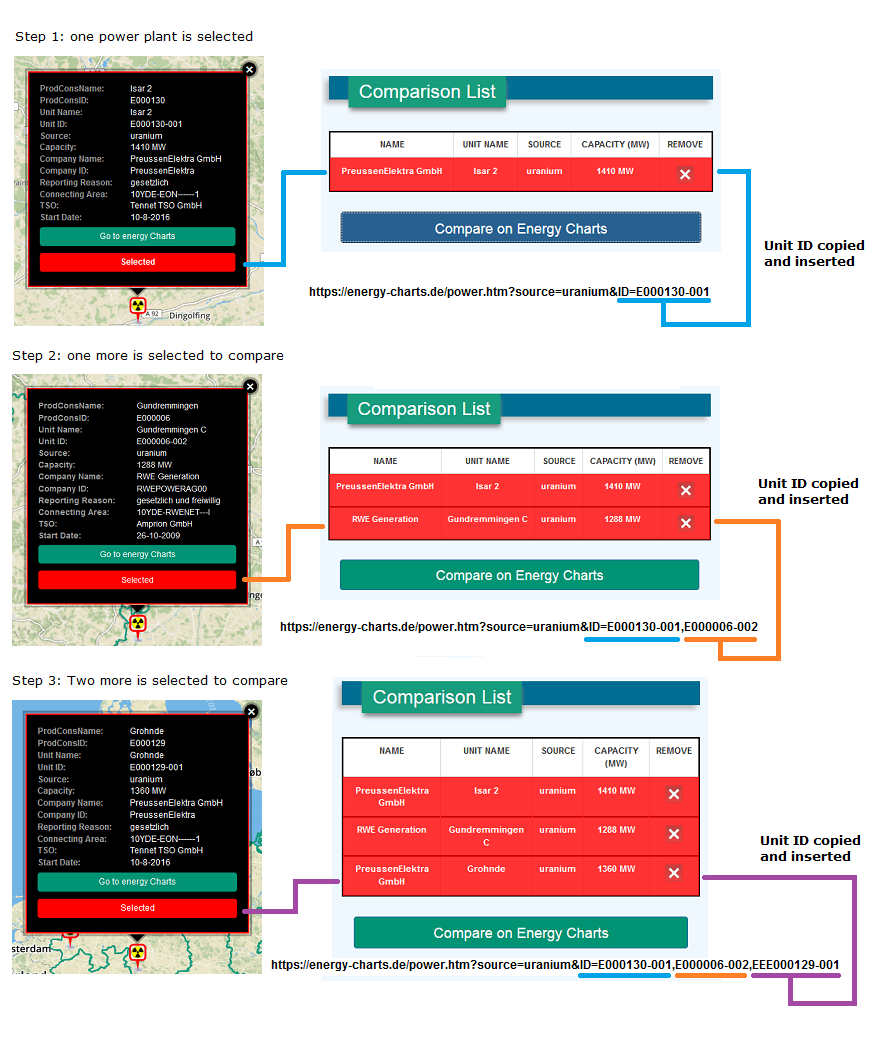
\includegraphics[width=1\textwidth]{multiplechart}
\caption[Steps of adding power plants to the comparison list]{Step 1: a nuclear plant is added into the comparison list - unit id added to the link; Step 2: another nuclear plant is added - new unit id added; Step 3: The last one is added into the list - unit id added and link is updated}
\label{fig:stepsPP}
\end{figure}

Electricity production data are all stored in JSON files. Charts always load the data dynamically and plot these files according to user selection. Every JSON file name is written in several parts. It has a unique source name, week and year. The week and year is manually set when the data for that particular week is available on the server. On having URL variables, energy chart uses these and creates the chart accordingly. URL variables are handled by JavaScript and stored it locally for further operation. “source” variable is used to select the radio button of that particular source category on the navigation menu and also to complete the filepath (see List \ref{lst:url-json}). Radio button initializes the filepath using the source name. List \ref{lst:url-json} shows an instance of the first step of handling URL variables. This operation is similar for both approaches. 

%[language=json,firstnumber=1]
\begin{Listing}
\begin{lstlisting}
var _unitID = []; // Empty array for storing ID from the link 
var _sourceName = getUrlVariables()["source"]; // Variable for storing the source name from the URL variables

_unitID = getUrlVariables()["ID"]; // get the ID/IDs from the link an stores inside this array

if (_sourceName != undefined && _unitID != undefined) { // checks if source and id are available inside the url

	var defaultradiob = "disp_"+ _new_sourceName; // Selects the radio button for selecting source

	var filepath = "./power_unit/week_"+ _path_source_name +"_"+ defaultyear +"_0"+ defaultweek +".json"; //file on first-load using link variables
}

\end{lstlisting}
\caption{URL variables are handled using JavaScript}
\label{lst:url-json}
\end{Listing}

\begin{figure}
\centering
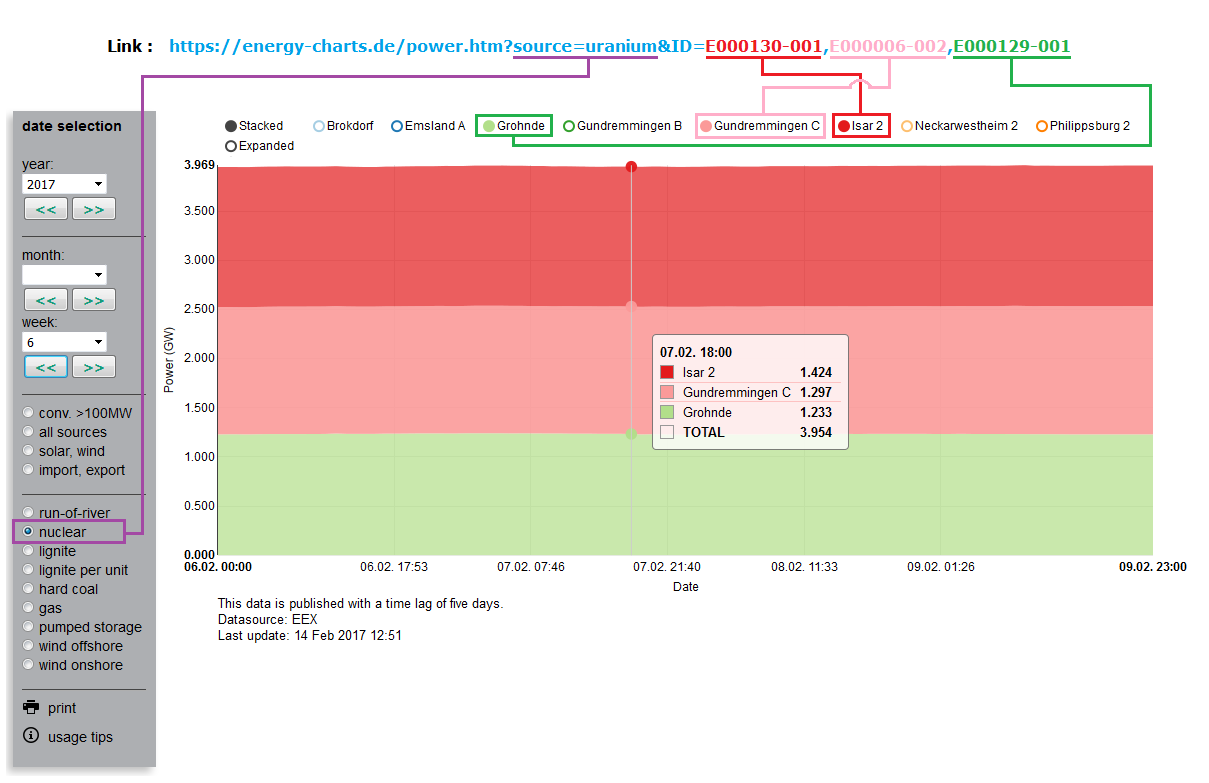
\includegraphics[width=1\textwidth]{ecselection}
\caption{Selected power plant data from the comparison table of Figure \ref{fig:stepsPP}}
\label{fig:ecselect}
\end{figure}

In the next step, algorithm handles unit ids from the URL. "Go to Energy Charts" link passes only a single unit id and "Compare on Energy Charts" link passes and array of unit ids. Figure \ref{fig:stepsPP} shows the impact of URL parameters to the electricity production chart. Source name from URL activates the radio button from the chart control area and unit ids are used to enable the visibility of those power plants on the chart. Therefore, circular legends are filled with colors. Other available power plant data is hidden from the chart thus circular legends are transparent. If there is no data available for selected units in JSON, then chart will load its default view instead. Default view of this chart enables the visibility of all power plants on the chart. 

%[language=javascript,firstnumber=1]
%\begin{Listing} [H]
%\begin{lstlisting}
%
%//Function for creating chart
%createChart(_sourceName, _unitID);
%
%function createChart(_sourceName, _unitID){
%	
%	// _sourceName is used for activating the radio button
%	_disp_source_unit = document.getElementById('radio button id').checked;  
%	
%	// _unitID is required here
%	if (_unitID != null) { // checks if unit ids is available on the URL
%		var uni_id = _unit_ID;
%		var query_list = []
%		query_list = uni_id.split(","); // array of unit ids - if more than one unit ids available //separate them using coma.
%	}
%	
%	// Function is ready for operation
%}
%
%\end{lstlisting}
%\caption{Function for creating chart with user defined parameter}
%\label{lst:createChart}
%\end{Listing}

NVD3\footnote{Official NVD3 Website, \url{https://nvd3.org/} (last accessed on \today)} JavaScript library has been used for creating chart on Energy-Charts page. It is a widely used charting library which is written in d3.js\footnote{Official D3 Website, \url{https://d3js.org/} (last accessed on \today)}. An instance of hourly production data file is shown in the List \ref{lst:dataFile}. This input JSON array has four attributes but only \textit{eexUnitID} is required to fulfill our requirements. The \textit{eexUnitID} of the hourly electricity production data and the unit id of the power plant location data (see Figure \ref{fig:stepsPP} are both the same ids. Our algorithm checks whether this eexUnitID exists inside the array of \textit{query list} or not. If exists then it is rendered on the chart. %List \ref{lst:algo} showing the JavaScript code for checking the URL parameter from the input data series.

%[language=JSON,firstnumber=1]
\begin{Listing} [H]
\begin{lstlisting}
// example of 
var inputData = [
{	"key": [{ "en":"Name_en" , "de":"Name_de" , "fr":"Name_fr" , "it":"Name_it" }] ,
	"color" : "rgb(number,number,number)" ,
	"eexUnitID" : "E000###-00#",
"KwNrBNetzA" : "BNA####" ,
	"values" : [ [ 1485903600000 , 0 ] , [ 1485907200000 , 0 ], [........]]}
]

\end{lstlisting}
\caption{Example of hourly production JSON data object}
\label{lst:dataFile}
\end{Listing}

%[language=JSON,firstnumber=1]
\begin{Listing} [H]
\begin{lstlisting}
IF link variables exists THEN
   IF Only one eexUnitID exsits THEN
     loop1: REPEAT UNTIL < query list length
     loop2:  REPEAT UNTIL < eexUnitID length
					IF eexUnitID exist in query list
        	          enable series visibility 
                	  BREAK loop1
                	end IF
					ELSE Disable series
			 END loop2
		    END loop1
   end IF
   ELSE //for more than one eexUnitID
     REPEAT REPEAT UNTIL < query list length
       IF eexUnitID exist in query list
         Enable Series
         BREAK loop2
       end IF
       ELSE Disable series
     END for
end IF

ELSE Enable Series
\end{lstlisting}
\caption[pseudo code for checking unit ids]{JavaScript pseudo code for checking unit ids and enabling their visibility on the charts}
\label{lst:algo}
\end{Listing}

This part of the code is the new contribution to the existing energy chart. Line 1 of List \ref{lst:algo} checks the existence of parameter on URL. This function runs if URL parameters are available. Line 2 checks the number of the URL parameter (less or greater than 1). If the type of \textit{ID} is object then starts executing from line 2. Conversely, the function starts executing from line 13 if the number of \textit{ID} elements are more than one. Subsequently, function repeatedly checks the availability of unit ids from URL inside the data series. For this purpose, Line 6 enables the visibility of that data series on the chart if its unit id matches whereas unmatched data series are disabled on line 9. After executing this code users get the actual desired data illustrated on the chart which were queried over the link.

\section{Interlinking the Energy Chart with the Map}

In Section \ref{sssec:connectivity}, the connectivity from the map to the energy chart is introduced where users can move to energy chart from the map to see the hourly electricity production of power plants. Likewise, an additional feature is imposed to the energy charts to establish a connection from energy-charts to the map. 

Energy chart users can locate the power plants on the interactive map. Firstly users need to select a source category to see their hourly production in the form of stacked are chart. After selecting a source from the navigation bar of energy chart, a button "Power plant locations" appears at the bottom of the chart. This button enables users to see the location of all power plants of the selected source. For example, a energy chart user is watching the electricity production of all gas power plant unit. Now the user is interested to see the locations of those power plants inside Germany. The locations of all gas power plant is shown on the map by clicking on "Power plant locations" (see Figure \ref{fig:interlink}). The function of this button is dynamically updated when user changes the source category from the navigation bar. 

\begin{figure}
\centering
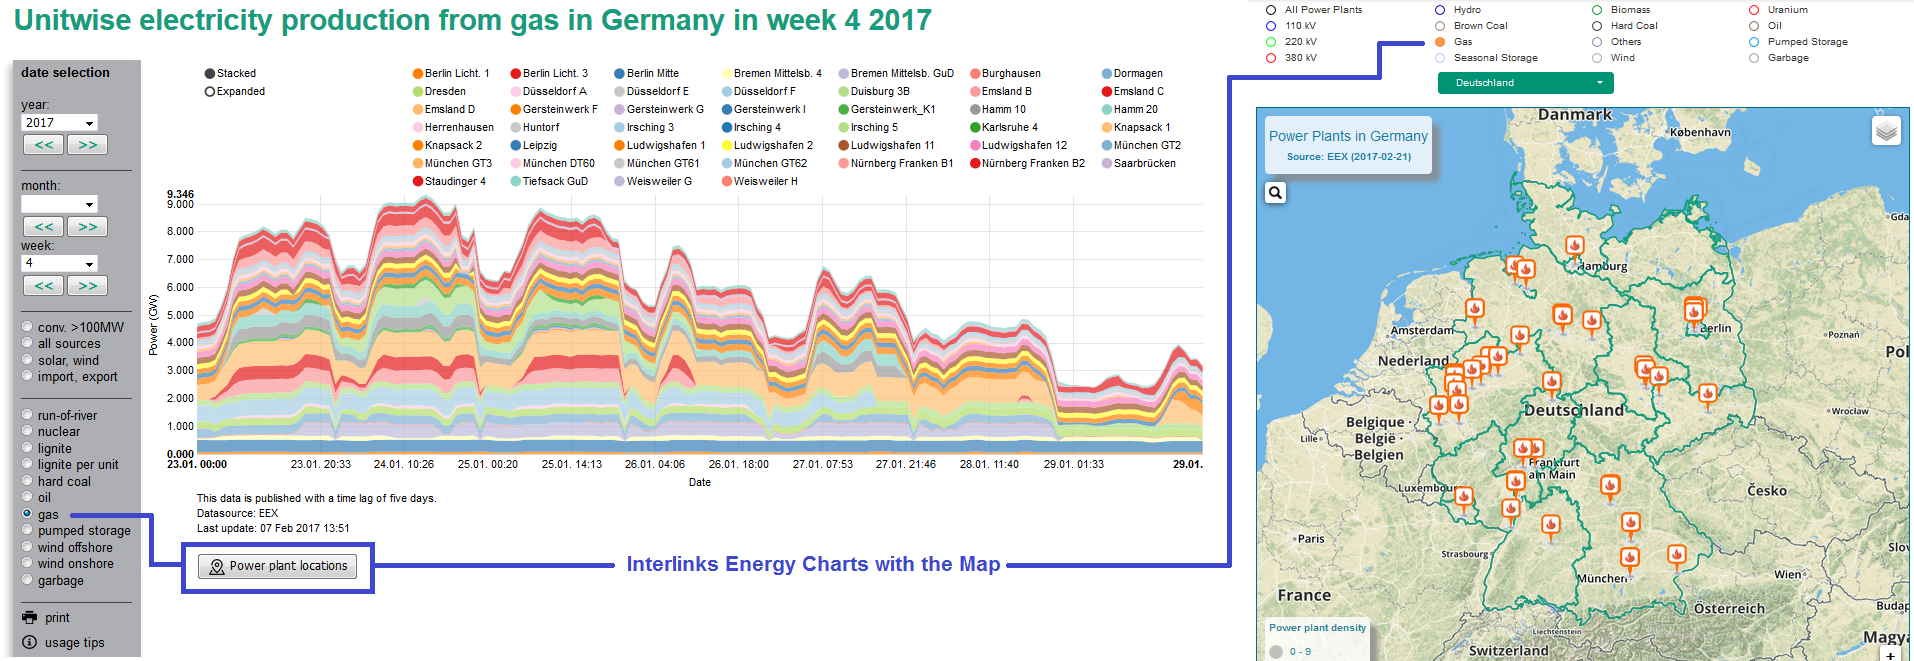
\includegraphics[width=1\textwidth]{interlinkButton}
\caption{Interlinking between energy charts and the map}
\label{fig:interlink}
\end{figure}

\section{Optimization of power line visualization}
\label{sec:powerLine}

In addition to the visualization of power plant location, showing the power transmission line is also a part of functional requirements. Therefore, our application provides an option for visualizing power transmission lines for 110kV, 220kV, and 380kV. Information about the data source is already discussed in Chapter~\ref{chap:background} Section \ref{sec:plsource}. Data was extracted in the format of geoJSON from the OpenStreetMap database. Figure \ref{fig:export} showing the available data formats that can be extracted using the overpass-turbo API. Leaflet supports GeoJSON and provides flexibility to map GeoJSON file there we have decided to use this format. Leaflet parses GeoJSON data and creates feature layers. Finally, the function displays the power transmission line to the map.

\begin{figure}
\centering
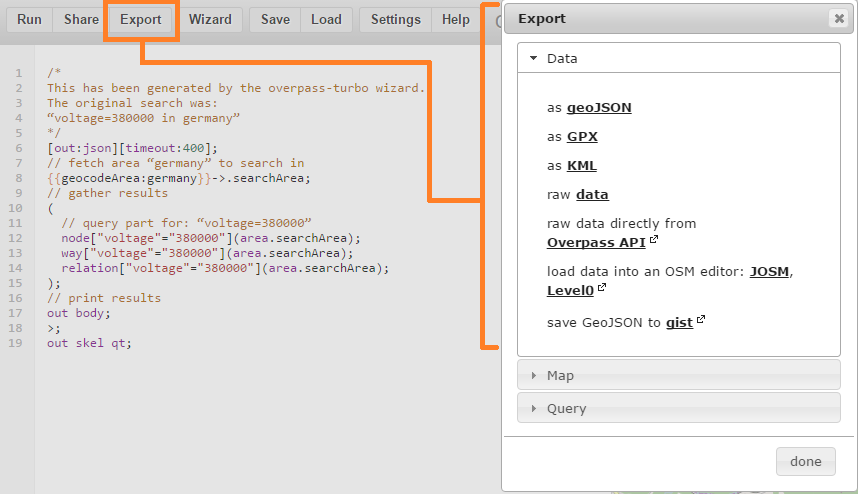
\includegraphics[width=1\textwidth]{export}
\caption{All possible data format that be extracted from the Overpass-turbo API}
\label{fig:export}
\end{figure}

The extracted GeoJSON data are too big in size. For the desktop computers it takes less than 2 seconds to load but Smart-phones and tablets take around 2 to 5 seconds for loading. Thus, it affects the performance of the map while zooming-in/out. Hence, it was required to optimize the process of mapping power lines. The following steps were taken to optimize the visualization of power lines.

\subsection{Map Bounds}

Leaflet provides extensive opportunities to control the map and provides current scale information about the map view. For our operation map bounds were considered for displaying the power transmission line on the map. It provides the lowest and highest value of latitude and longitude of the map view. Map bounds are changed every time the map is moved (either by zoom or pan).  Therefore, we used a function to reconsider the map bounds in every zoom level and display the GeoJSON data accordingly. Each time the map is moved, the map bounds is stored. If the power line data contains the map bound then the line is displayed otherwise it is skipped from mapping. Figure \ref{fig:mpbound} showing the power lines (380 kV) on 2 different zoom levels. In figure \ref{fig:mapBoundG}, map zoom level is 6 and whole Germany is visible inside the map bounds. Therefore, all the power lines data contains inside the current map bounds. Figure \ref{fig:mapBoundB} represents the map on zoom level 8 and showing the power lines that contains inside the current map bounds. Every time the map is moved, power lines are update according to the map bound. The Power lines which are outside the map bounds are skipped from operation. As a result, performance of the map was improved and loading time of the power lines were faster than before. List \ref{lst:plBound} showing the pseudo code for filtering the power line by utilizing the map bounds. Line 1 checks if the map has moved or zoomed-in/out and line 2 checks whether any power line is selected by users. A function for updating the power lines is called in line 4. Map update function is represented between line 8 to line 14 which is doing the filtering operation and return the layer to the map. 

\begin{figure}
  \begin{center}
\subfloat[Complete 380kV power line in the Germany (zoom level 6, no filtering)\label{fig:mapBoundG}]
  {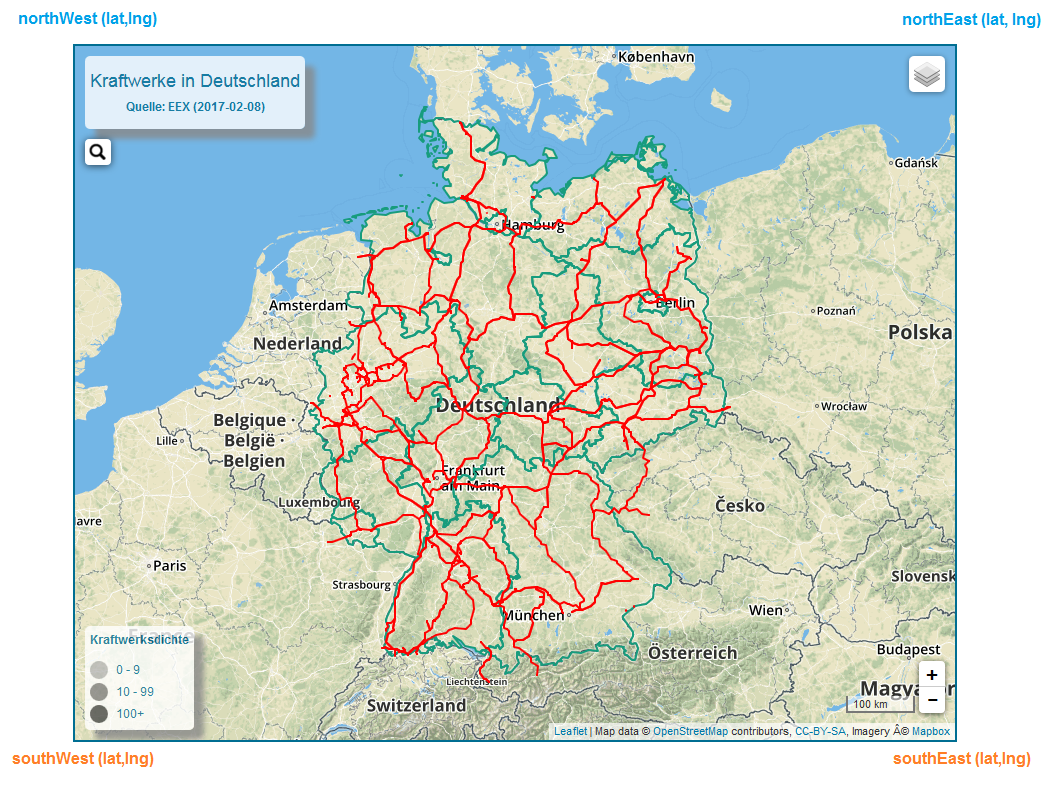
\includegraphics[width=.45\linewidth]{mapBoundGermany}}\hfill
\subfloat[380kv power line through Berlin (zoom level 8, filtered by map bounds)\label{fig:mapBoundB}]
  {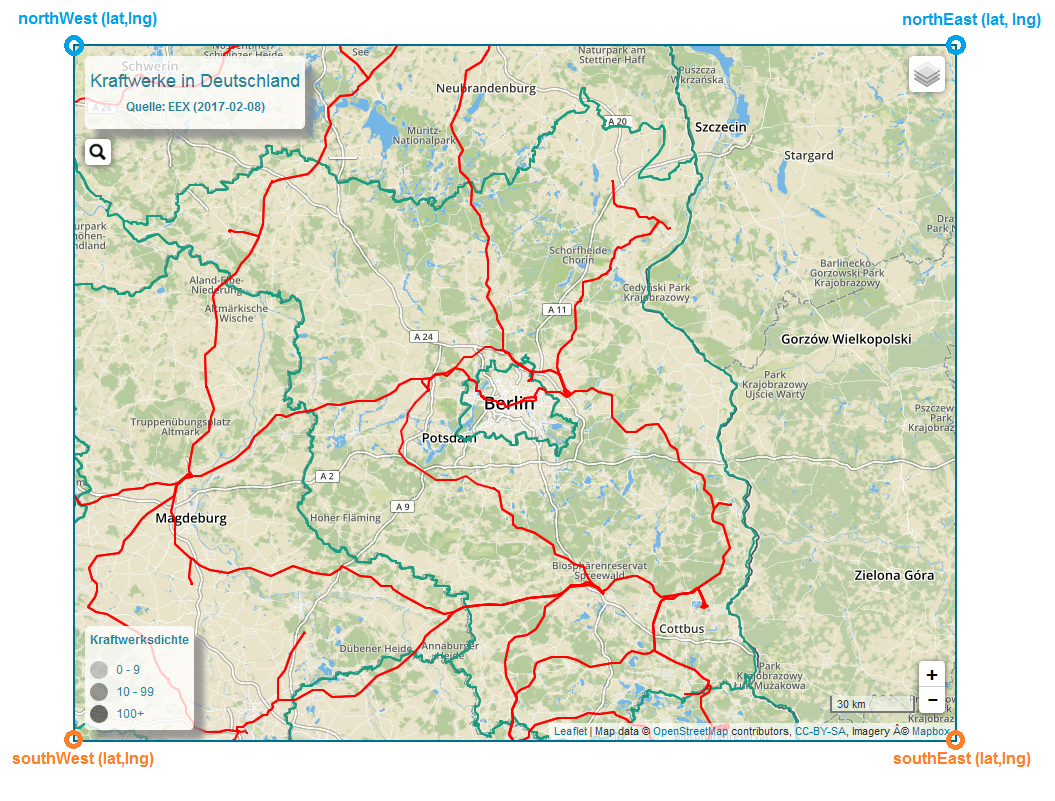
\includegraphics[width=.45\linewidth]{mapBound}}
\hfill
\caption{Filtering power lines depending on the map bounds}
\label{fig:mpbound}
\end{center}
\end{figure}

%[language=JavaScript,firstnumber=1]
\begin{Listing}
\begin{lstlisting}
ON map move ends or map zooming ends
	IF power line input selected
			DO remove previous layer
			CALL updateMap function
			DO add new power line layer
	end IF
// function for updating the map
FUNCTION updateMap
			GET map bounds
			CREATE power line layer
				IF layer contains map bounds
					ADD to layer
					RETURN layer
			end IF
\end{lstlisting}
\caption{Power line filtering algorithm depending on the map bound}
\label{lst:plBound}
\end{Listing}

\subsection{The Length of Power line}

The length of power transmission line is also considered for optimization. A long power transmission line is a collection of small sub layers of line string. These smaller line strings are affecting the performance of the map while loading.  For this purpose, smaller power lines are hidden on smaller zoom levels (when zoom level <= 8).  Small power lines contain a length between 1m to 500m. These smaller power lines are visible on higher zoom level ( zoom level > 8). This optimization is applied only for the 110kV power line. 110kV geoJSON data is relatively bigger in size and has more details than 220kV and 380kV transmission lines. 

This file has massive amount of entries for power lines and power stations. Polygons are describing mostly the power stations or substations inside the GeoJSON data and line-strings are describing the power transmission line. To visualize the proper routing and angle of power lines on the map, they are divided into many smaller parts inside the GeoJSON file. Our algorithm is hiding the power stations or substation, which are polygons, in smaller zoom level. Because, this smaller entries doesn't provide any useful feedback to the user. These smaller lines are available and added to the map on higher zoom level. Figure \ref{fig:plfilter} showing the power line density on different zoom levels. In figure \ref{fig:pl6}, power lines with smaller coordinate length (length > 45) are hidden where in figure \ref{fig:pl8} those lines have coordinate length less than 20 are hidden. The complete data information on 110 kV power lines are available when zoom level is higher than 9. Substations and smaller power transmission lines can be recognized at this zoom level. 

\begin{figure}
  \begin{center}
\subfloat[100kV power line (zoom level<6, coordinate length > 45)\label{fig:pl6}]
  {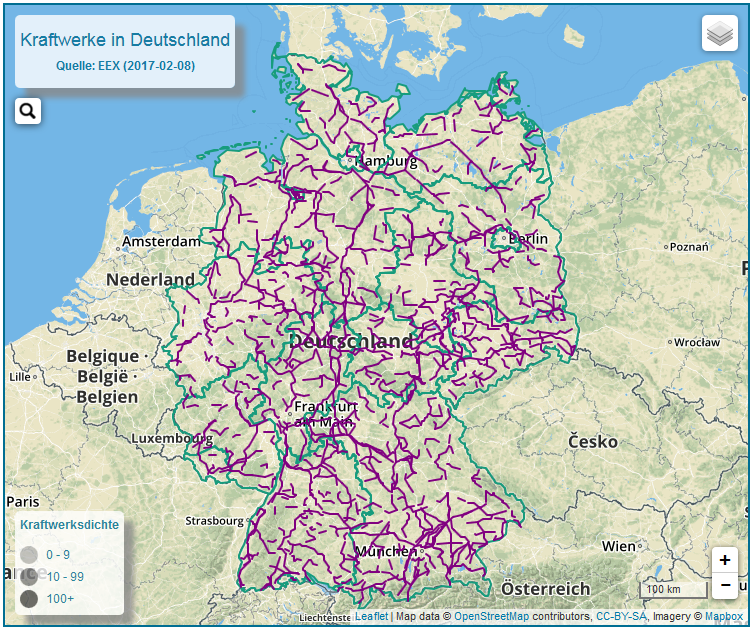
\includegraphics[width=.45\linewidth]{plzoom6}}\hfill
\subfloat[100kV power line (zoom level 8, coordinate length > 20)\label{fig:pl8}]
  {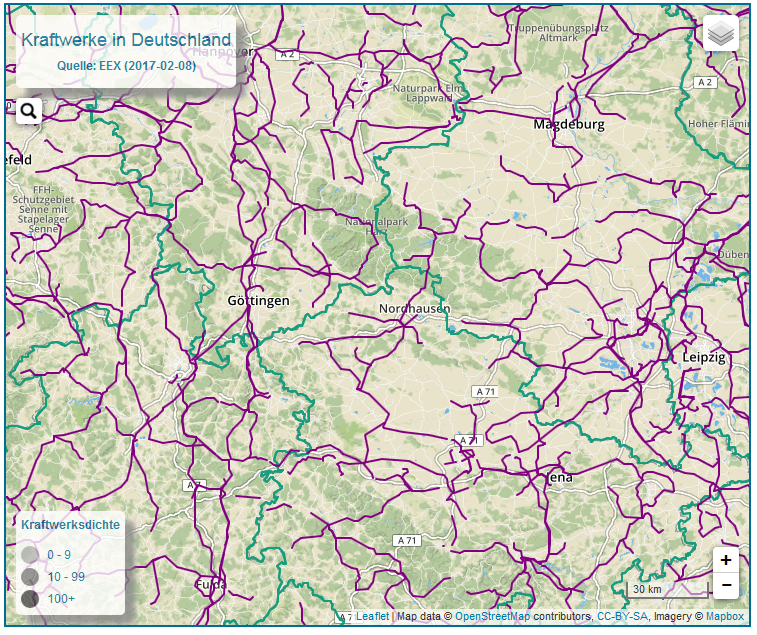
\includegraphics[width=.45\linewidth]{plzoom8}}
\hfill
\caption{Filtering power lines by coordinate length}
\label{fig:plfilter}
\end{center}
\end{figure}

\section{Summary and Discussion}

In this chapter, the implementation of the back-end and the front-end of the system was explained.
Furthermore, an overview of the graphical user interface as well as a detailed impression of
the architecture , interactivity scripting , interconnection process between map and chart was given. The visualization application solves the interface and functional requirements described in the Section \ref{sec:reqAn}. User are able to locate power plants and their hourly production data on energy chart. Furthermore, we assume that our visualization tool will help user to access the information of power plants as well as their hourly electricity production data. 

\chapter{Evaluation}
\label{chap:evaluation}

The online interactive map was evaluated in two different studies. Beforehand, it was published online and merged to the existing energy chart website to make it available for the large audience. In addition, an online survey was prepared to evaluate the map and deployed online to assess the impact, usefulness, and usability of the of this visualization tool.  This online study evaluates the map on two different characteristics. The first study was focusing on the representational aspects of the map and the second was aiming at the usability of the map and its interactive functionality. The goal of this survey was to accumulate qualitative feedback on the map interface, visualization techniques, usability, and scopes of accessing data. A wide range of users assessed the survey. Some of them were from the field of renewable energy study and research, university professors, engineers, journalist, public service holders, businessman, and students. In this chapter, the survey studies and their results are analyzed, explained, and discussed in detail.

\section{Online survey setup}
\label{chap:suveySetup}

The online survey evaluation process was divided into four different question groups with a brief introduction about the purpose of this evaluation and a little usage guide of the visualization tool. Therefore, users can explore the map and discover the functionality before participating in the survey. The participants were invited over the email and social media. They did not get any reward for participating in the online survey. None of the survey questions were mandatory, therefore participants were not required to answer every question. 

In the short introduction, all the participants were informed about the purpose of making this visualization tool followed by a short description about the usability, and some tasks they need to perform for using the map and accessing the data out of it. The tasks were divided into the following steps:

\textbf{Exploring power plant information:}\\
In the description, participants were asked to click on the map marker to view the information of each power plants from the pop-up box. 


\textbf{Use navigation menu for interaction:}\\
In the description, participants were told to use the navigation menu for selecting each source category and for rendering the power lines on the map.

\textbf{View hourly production data:}\\
In the description, participants were told to use the “Go to Energy Charts” link to view the hourly production data on the energy charts.

\textbf{Compare power plants production:}\\
In the description, participants were told to compare between power plants in a comparison table by using the “Compare” button from the pop-up box.

\textbf{View hourly production data of multiple power plants:}\\
In the description, participants were told to use “Compare on Energy Charts” link to see the production data of the power plants in the comparison list. 

After the short introduction, some questions were asked to the participant to empirically evaluate the interface and usability of the map. In total 20 questions were asked to the survey participants and participation time was estimated about 5 minutes.  

\subsection{Question groups}
\label{sssec:quesGroup} 

\subsection*{Introduction}
\label{sssec:intro}

The first question group was about the self-introduction. Participants were asked to mention their gender, age, and professional area of working, besides that their frequency of using interactive maps and their acquaintance with the German power plants and its electricity production were asked. 

\subsection*{User Interface evaluation}
\label{sssec:uiEval}

In this group, participants were asked to evaluate the user interface and its components especially about the cluster view, map markers, power lines, and comparison table. A collection of the demographic question, rating scale, and multiple choice question were asked for this evaluation. 

\subsection*{Map Usability test}
\label{sssec:MUtest}

In this group, participants were asked to evaluate the usability and usefulness of this visualization tool. Participants were also requested to leave some comments if they found the tool difficult to use. 

\subsection*{Comments or Suggestion}
\label{sssec:cORS}

Participants were asked to comment on this complete work package and its features as well as requested to provide suggestions on adding new features or ideas.  

\section{Survey Results and Discussion}

In this section, the result of survey questionnaire of each question group and the qualitative comments and consequences derived from these visions are discussed. 

\subsection{Summary of participants and their backgrounds}

The goal of this question group was to get an idea about the participants, their professional background, age ratio, and their familiarity with German power plants. In addition, how frequently they use interactive maps in their daily life. For our online research study, 23 participants (19 males, 2 females, 2 did not answer) from different level expertise participated in the survey. Participants belong to different age groups where 50\% with an average age of 27 years, 35\% are with an average of 53 years and 15\% are with an average age of 36 years (see Figure \ref{fig:participantBack}). In total, 19 full and 4 partial survey reports were submitted. 

\begin{figure} [H]
  \begin{center}
\subfloat[Age ratio of participants\label{fig:age}]
  {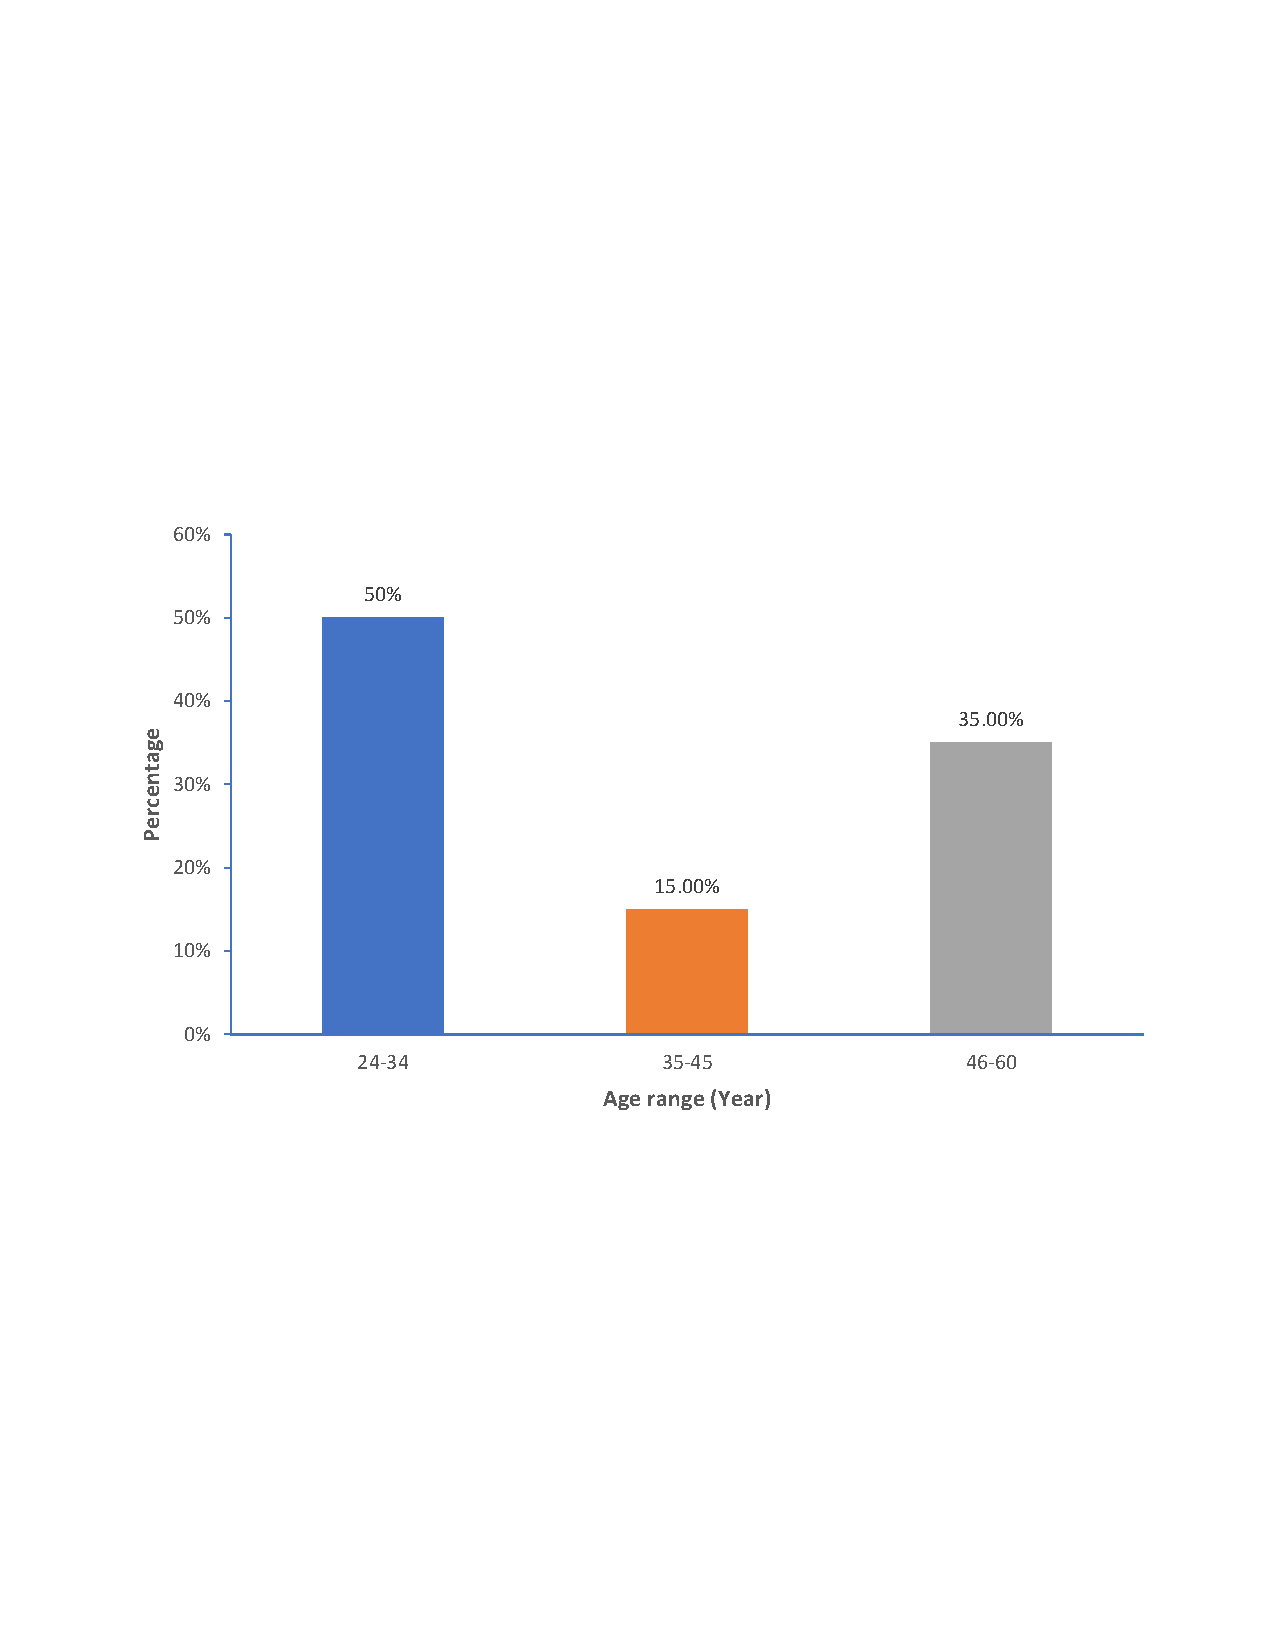
\includegraphics[width=.45\linewidth]{study/age}}\hfill
\subfloat[Professional backgroud of survey participants\label{fig:ageJob}]
  {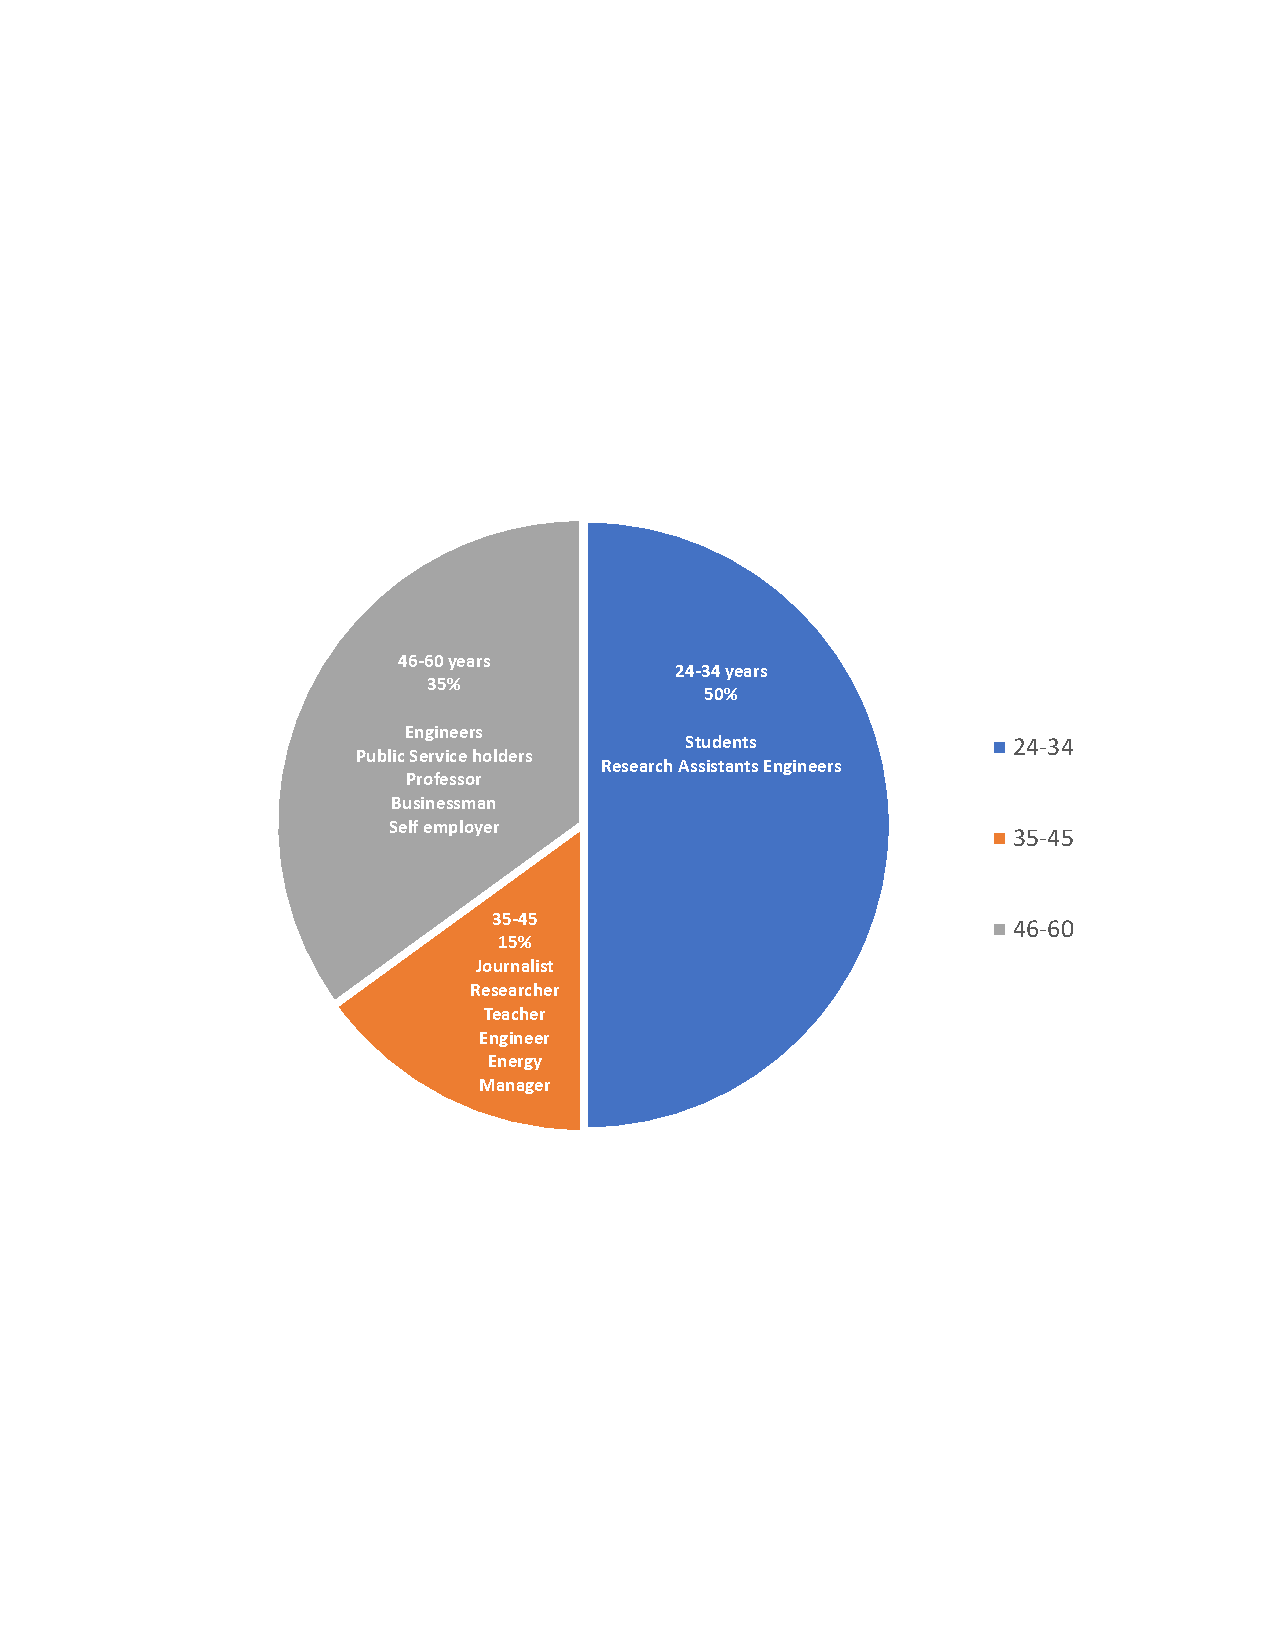
\includegraphics[width=.45\linewidth]{study/pie}}
\hfill
\caption{Age ration and professional background of survey participants}
\label{fig:participantBack}
\end{center}
\end{figure}

Summary of this question groups tells us that almost 50\% of the participants who are comparatively younger than other participants are familiar with German power plants and their production to some extent whereas other participants, who belong to older age groups, are somewhat or very much familiar with it (see Figure \ref{fig:familiar}). After digging up the data more deeply it has been noticed that younger participants are mostly students, research assistants, and engineers however participants older than other group are professors, businessman, and working in the energy industry. Nevertheless, the participants having no idea about German power plants also exists in all age groups. On the other hands, concerning the frequency of using interactive map per week, a maximum number of participants (around 70\%, see Figure \ref{fig:mapUsage}) use interactive map at least once or twice in a week. Therefore, we assumed that user would find the tool and its functionality easy to use.

\begin{figure}
  \begin{center}
    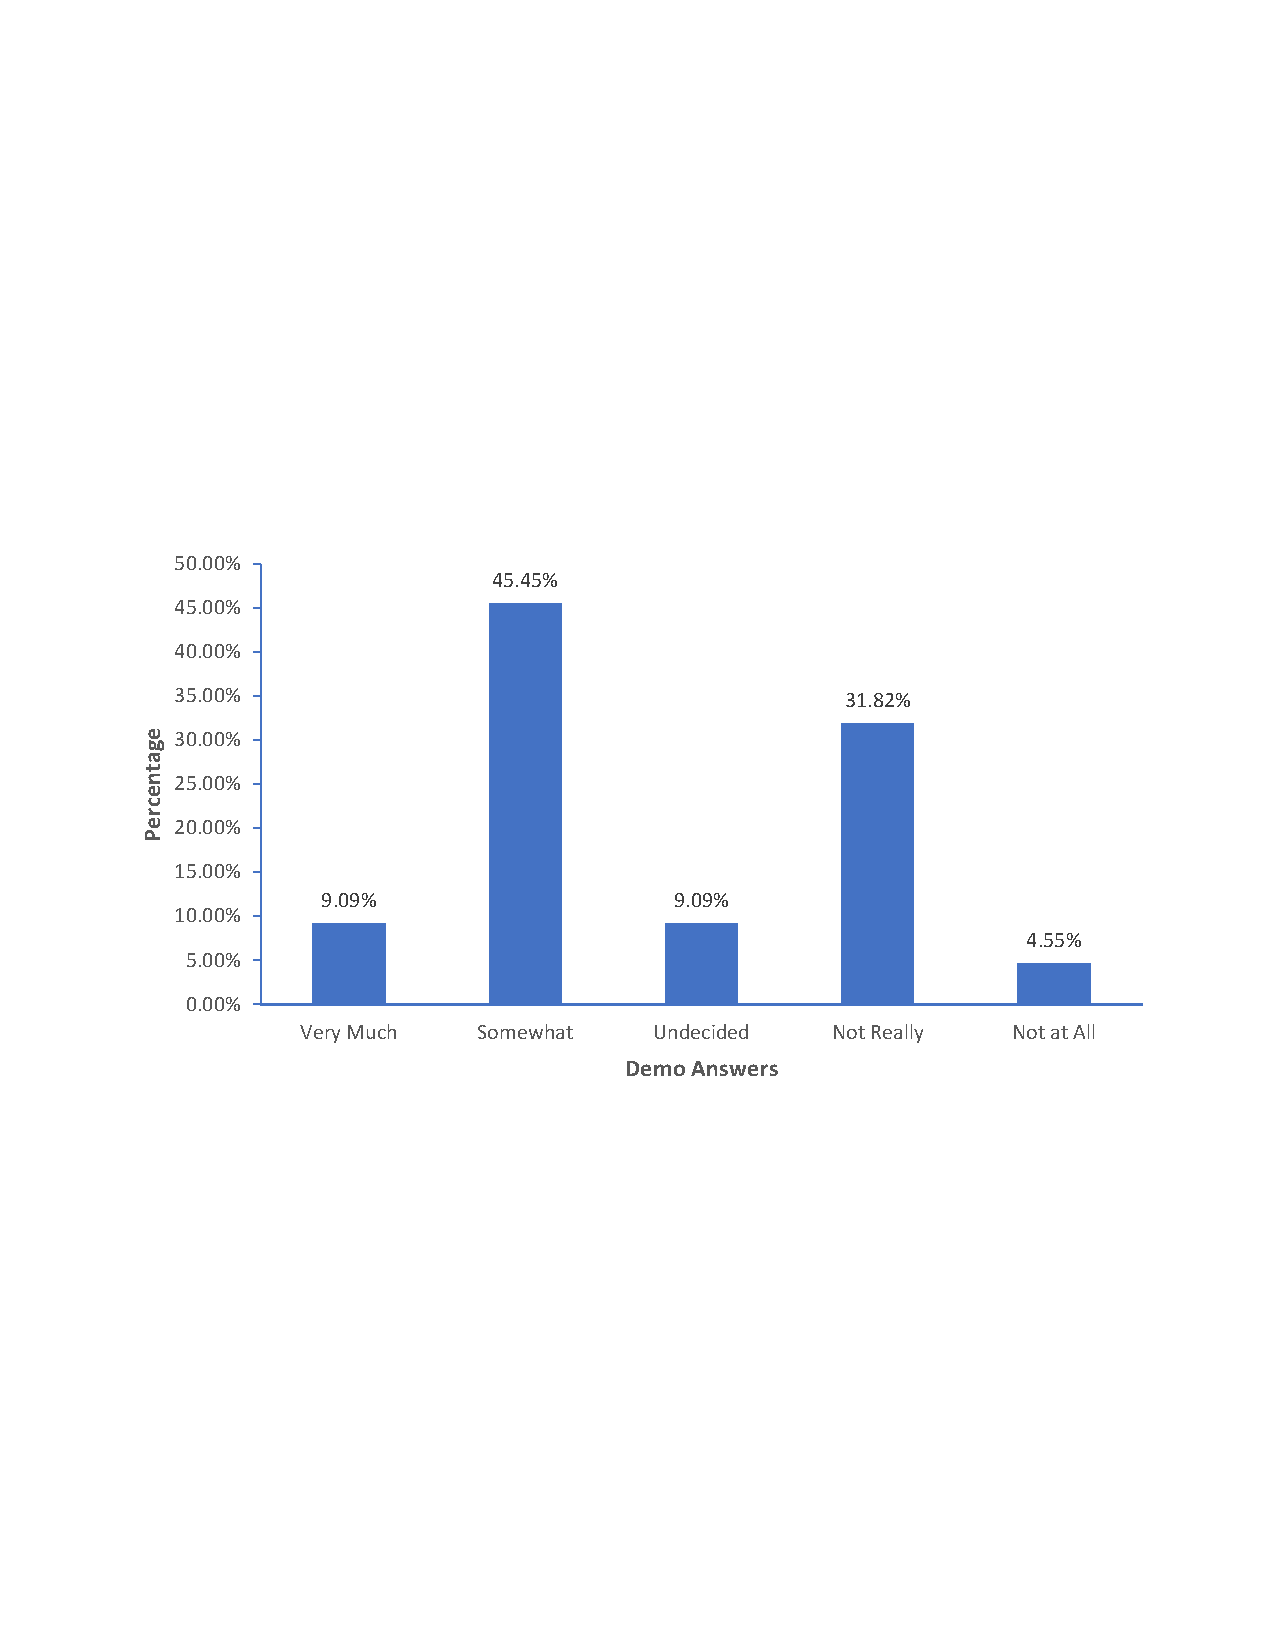
\includegraphics[width=1\textwidth]{study/familiar}
    \caption{Familiarity with German power plants and their production}
    \label{fig:familiar}
  \end{center}
\end{figure}

\begin{figure} 
  \begin{center}
    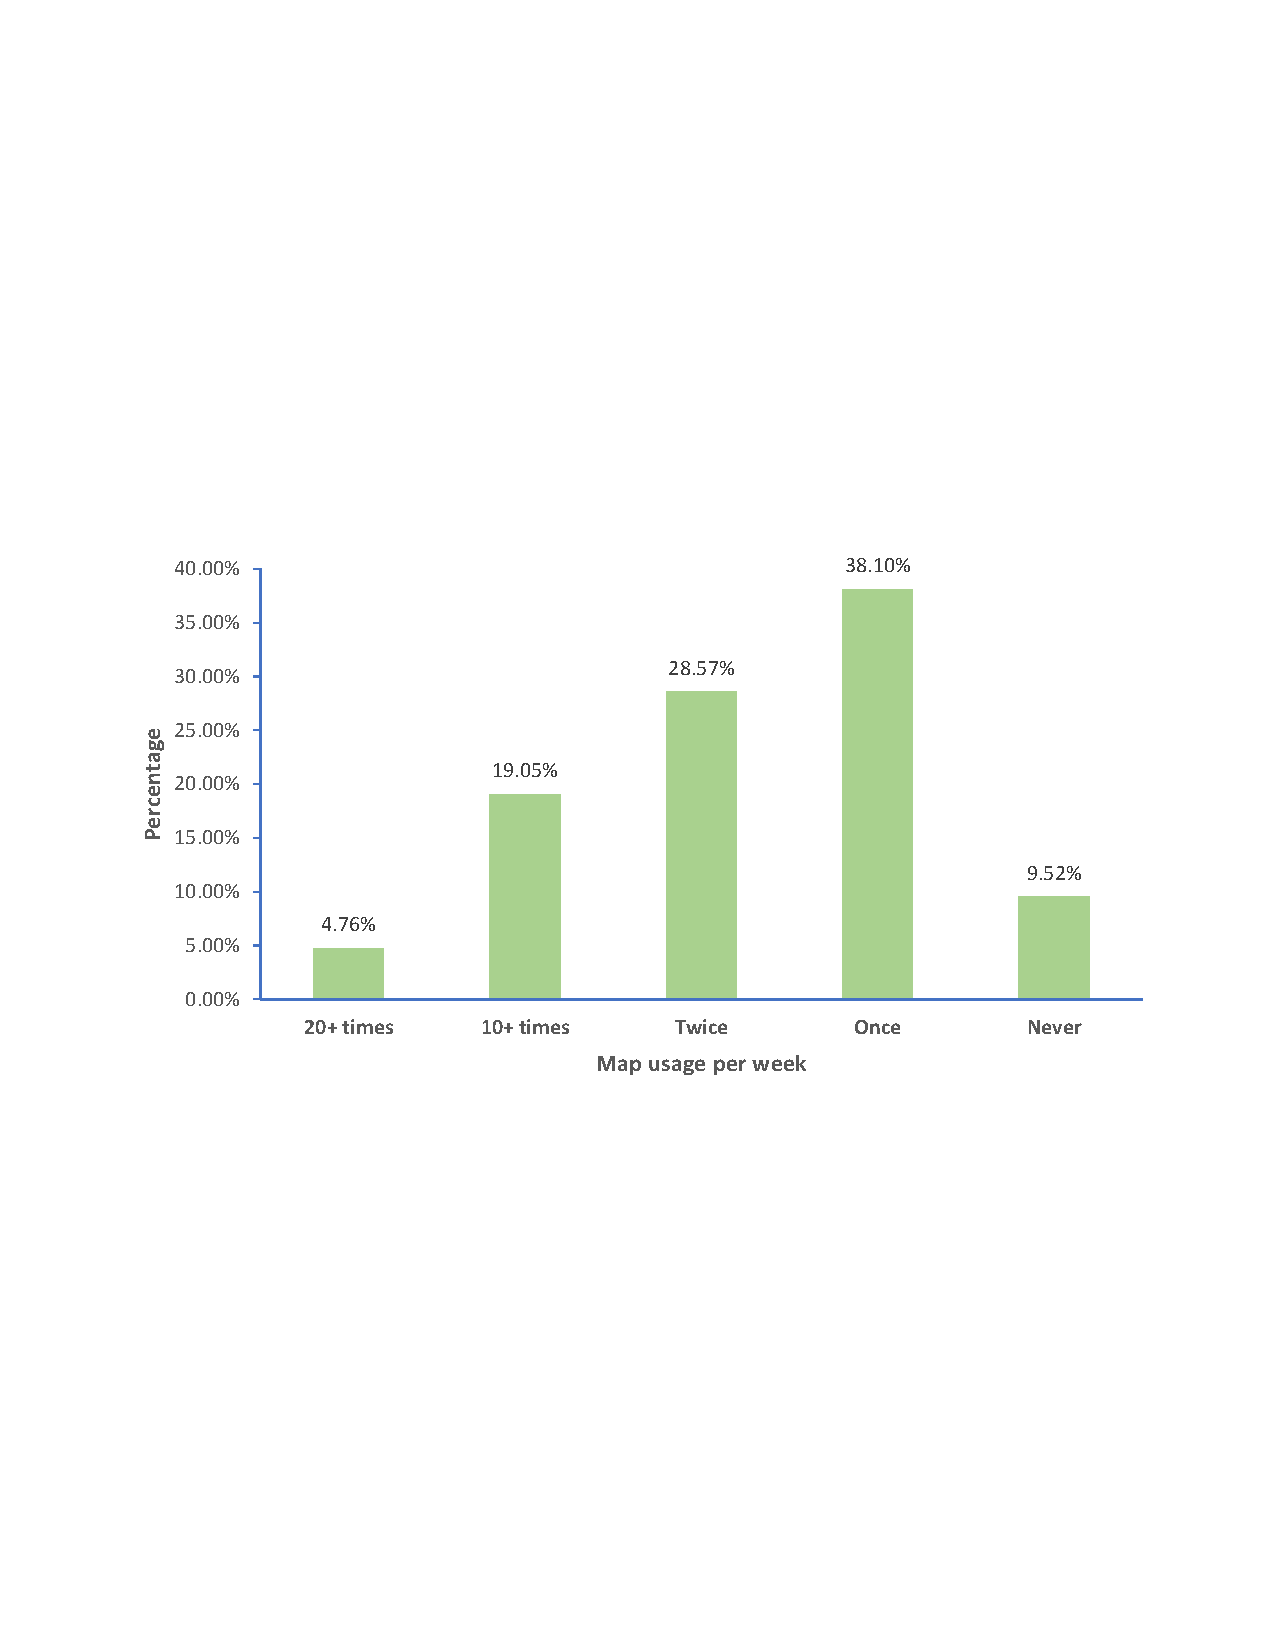
\includegraphics[width=1\textwidth]{study/frequency}
    \caption{The result of online survey - participants frequency of using interactive map per week}
    \label{fig:mapUsage}
  \end{center}
\end{figure}

\begin{figure}
  \begin{center}
    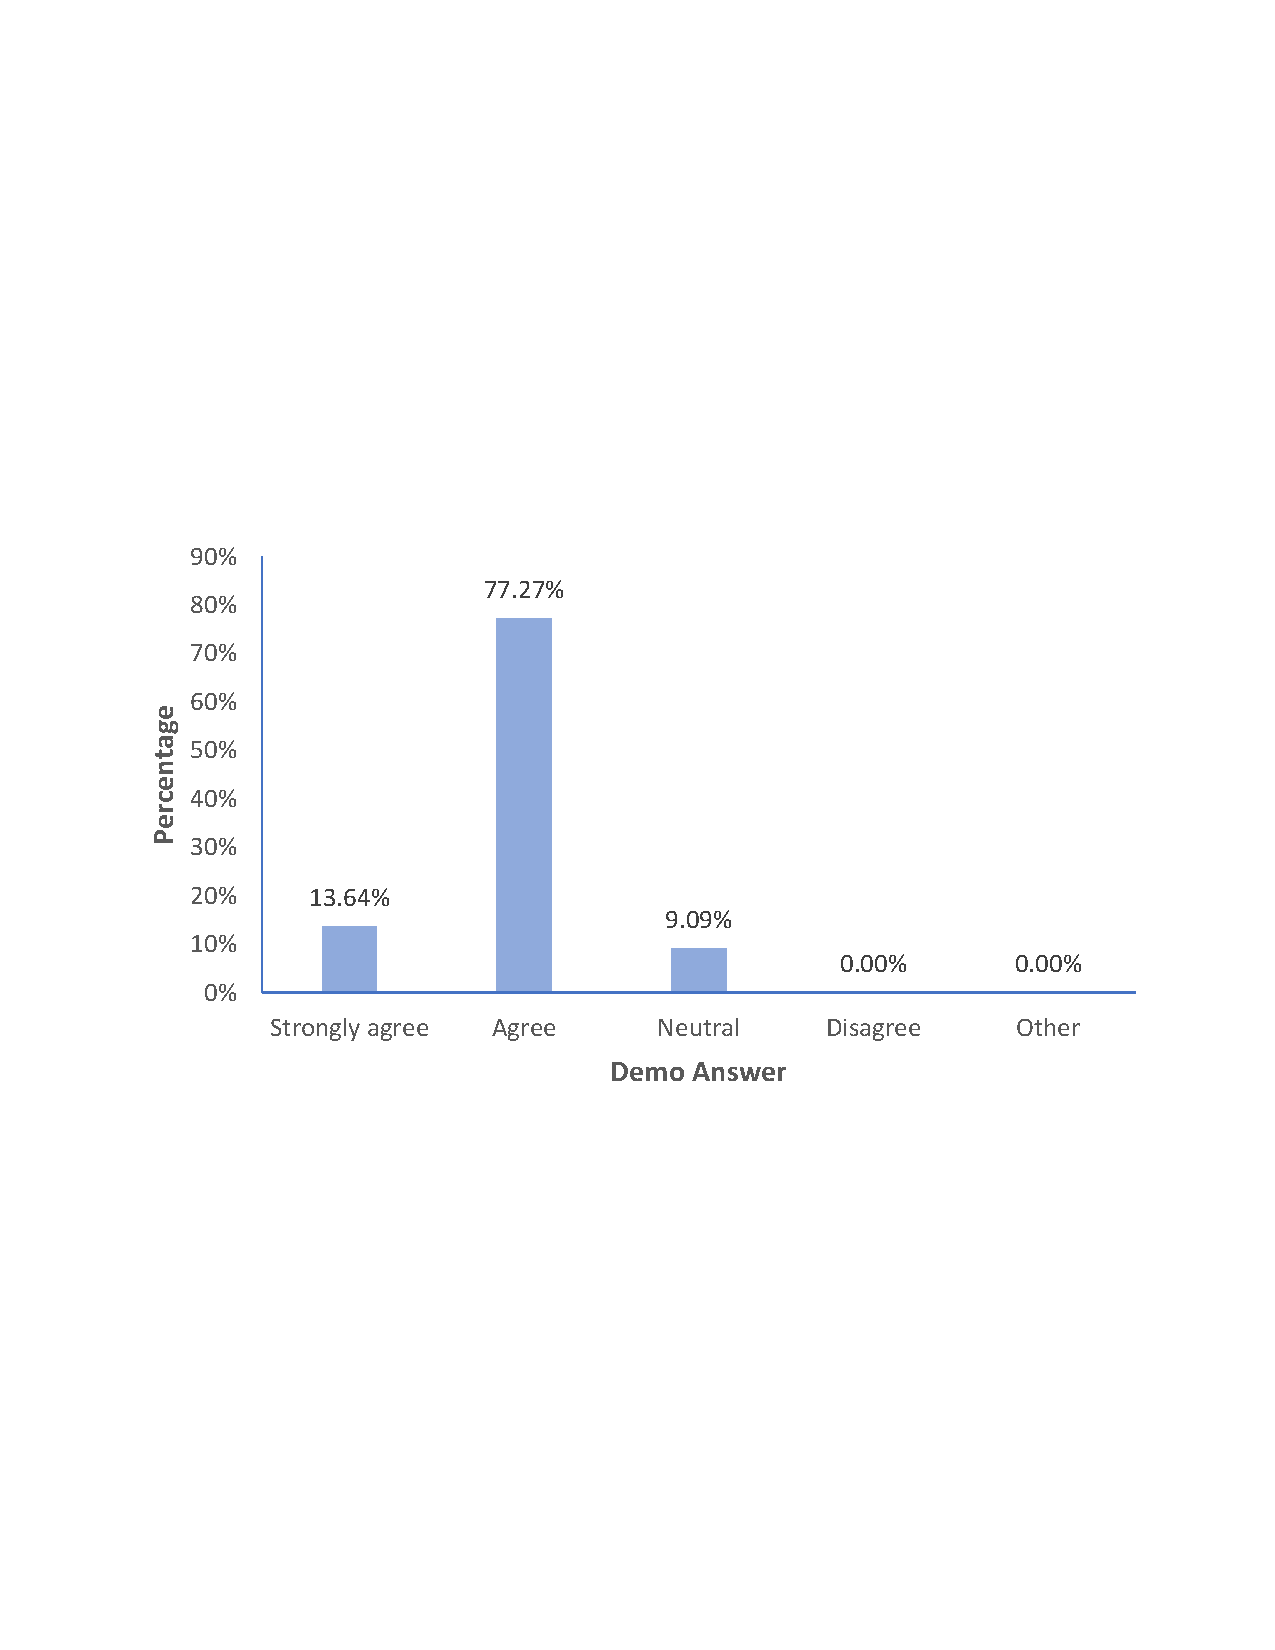
\includegraphics[width=1\textwidth]{study/etu.pdf}
    \caption{The result of online survey - map usability}
    \label{fig:etu}
  \end{center}
\end{figure}

\begin{figure}
  \begin{center}
\subfloat[The evaluation result of map usability by participants\label{fig:etu}]
  {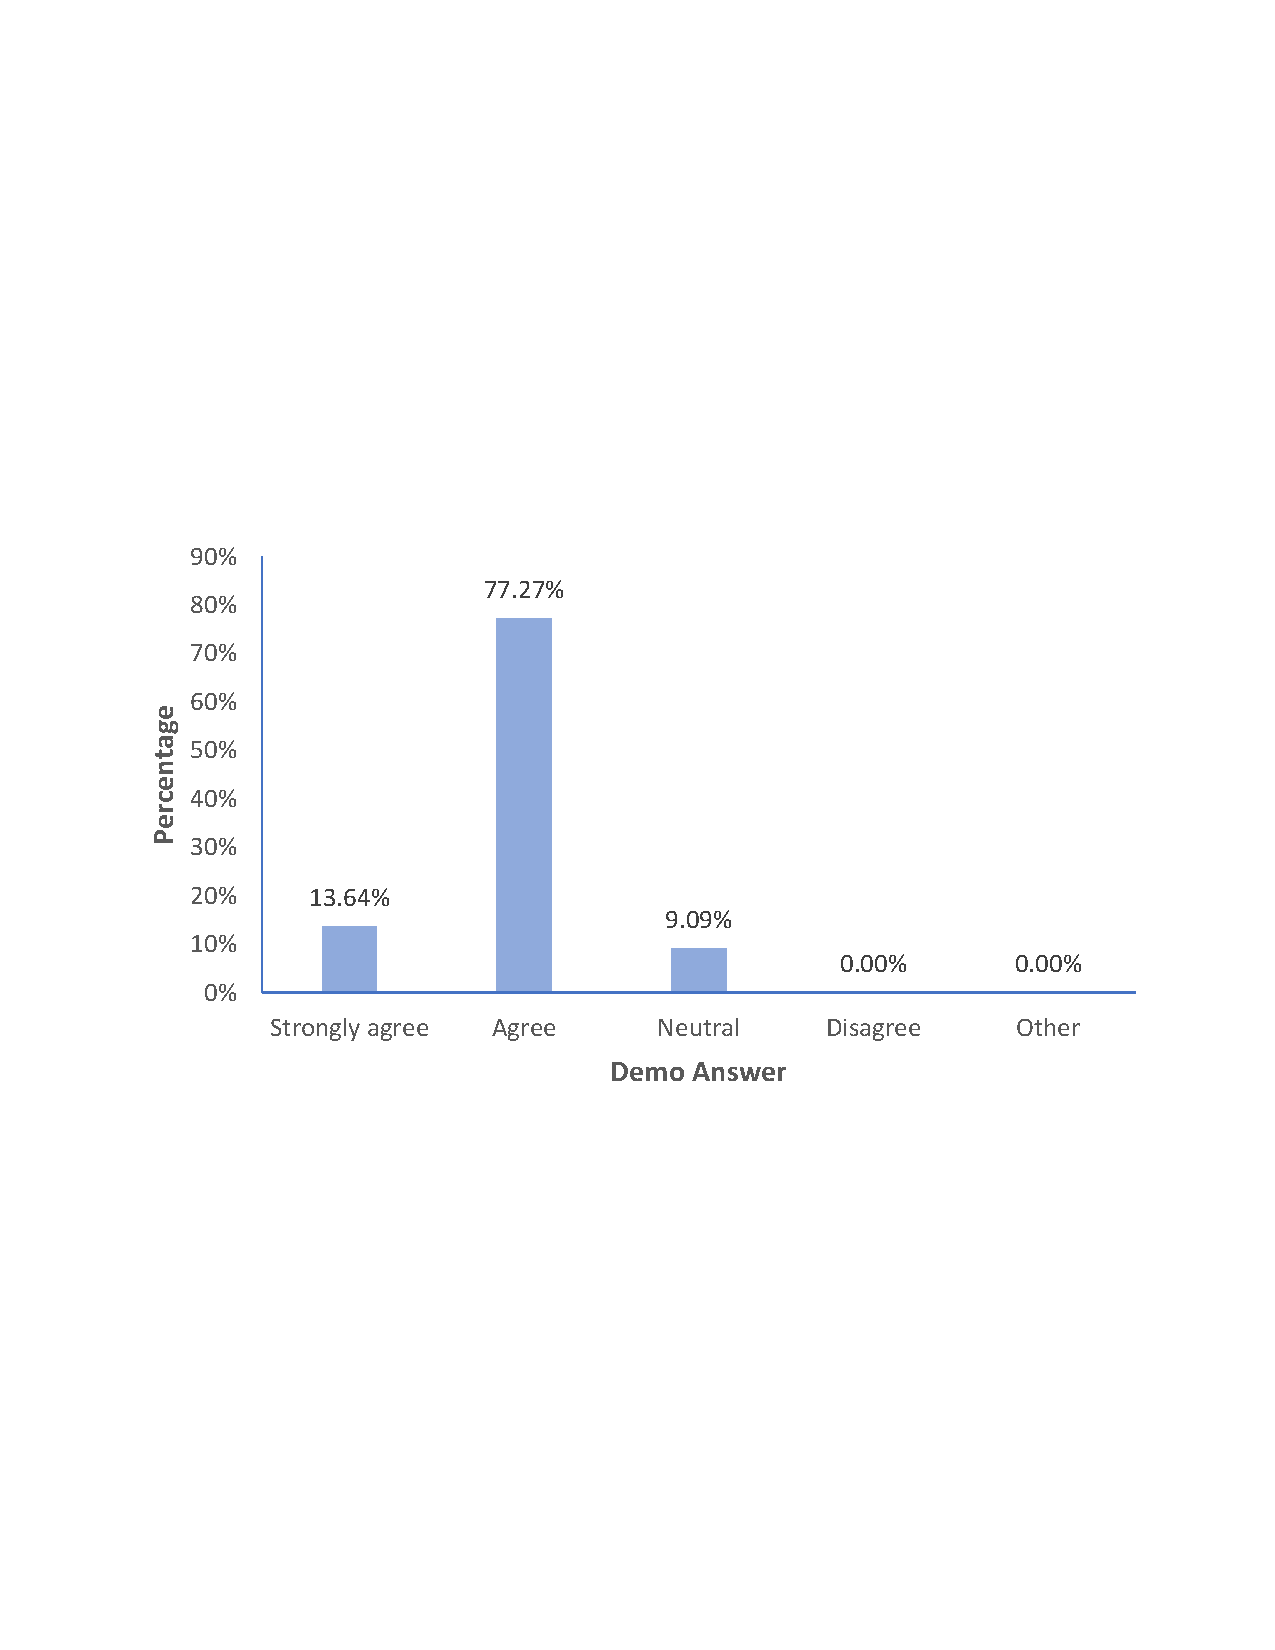
\includegraphics[width=.45\linewidth]{study/etu.pdf}}\hfill
\subfloat[The evaluation result of interface and functionality by participants\label{fig:selfExp}]
  {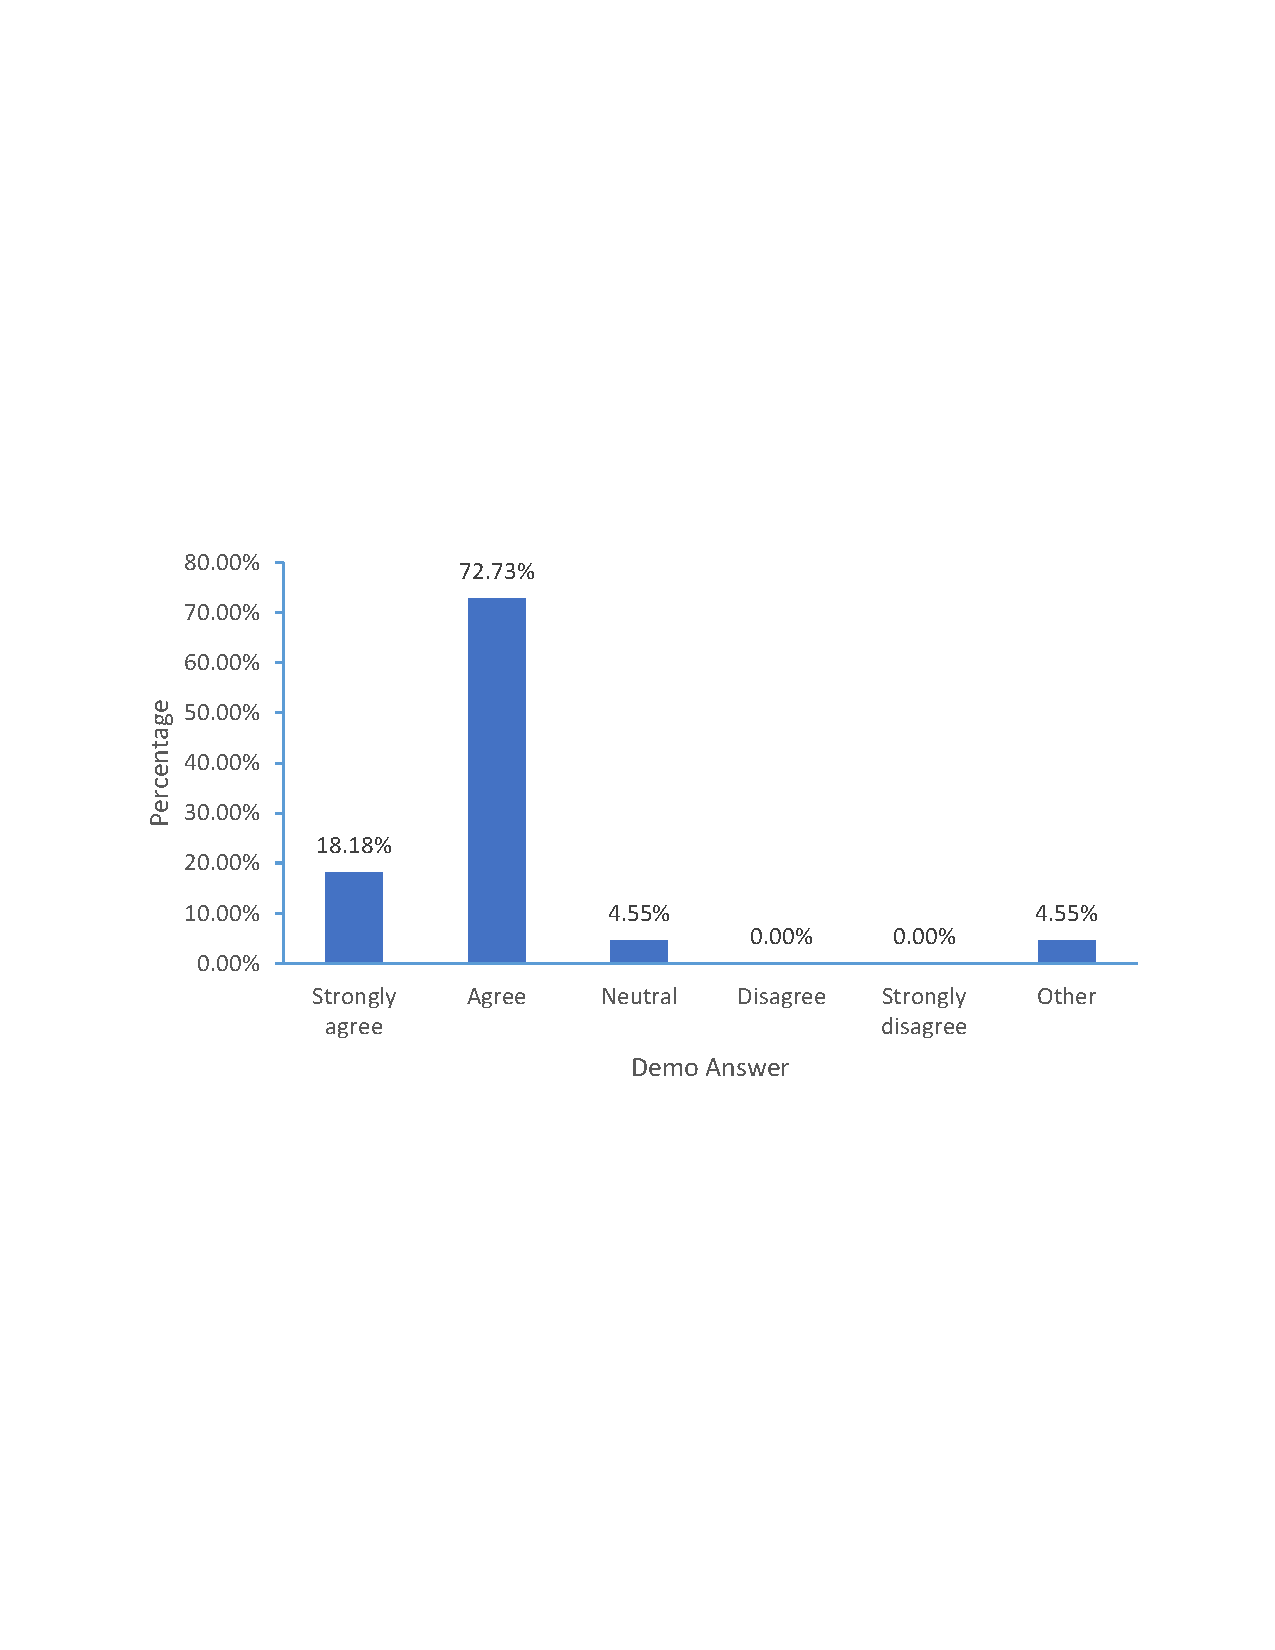
\includegraphics[width=.45\linewidth]{study/selfexp.pdf}}
\hfill
\caption{The evaluation result of online survey}
\label{fig:selfExp}
\end{center}
\end{figure}


\subsection{Working with the Interactive Map}

\subsection*{Evaluation of User Interface(UI)}

We assumed that before evaluating the UI, user followed the steps described in the short introduction and gone through the interface accordingly. The purpose of this questionnaire was to evaluate the map UI and its complexity, comprehensibility, construction as well as visual aesthetics. The participants were very positive after using the map and its interface. They found it intuitive and easy to use which is confirmed by the around 91\% participants. Where 77.27\% participants were agreed and around 13.64\% were strongly agreed on the question \textit{“I found the map easy to use”} of the survey (see Figure \ref{fig:etu}). Similar results are also noticed where participants were asked about the structure of map especially the navigation menus, markers, marker pop-ups, buttons, and comparison table. This is shown by the of 91\% (about 72.73\% agreed and 18.18\% strongly agreed) participants on the question \textit{"Interface and functions of this map are self-explanatory"} of the survey (see Figure \ref{fig:selfExp}). There was also a comment section where participants can write about their confusions instead of answering the question. P12 (a participant) took this opportunity and wrote, \textit{"Definitely they are self-explanatory.”}. P2 said, \textit{"navigation menu could have a logo next to each label”}.

\subsection*{Evaluation of Map API}

The participants rated the initial cluster by the average score of 3.81 (Standard deviation = 1.40, lowest(strongly disagree) – 1.0, highest – 5.0(strongly agree). This score falls between neutral and agree. A mixed response from the participants on the cluster view is noticed from the high standard deviation. Some of them found it interesting but at the same time, some found it confusing and unnecessary. P12 again commented, \textit{“The power plant density function should be removed, it is only confusing”}. P13 noted the cluster view appears on higher zoom level and said, \textit{“The power plant density representation is not always helping, its appearance can be resolved at higher zoom level”}. The Participants found the size of the marker \textit{“Just right”} although some participants found it little bigger. They were satisfied with the icons used inside the marker. The question \textit{“Icons used for power plants are self-explanatory”} got an average score of 4.13 (SD =0.71). Participants also rated the readability of the marker pop-up by the average value of 3.9 (Standard deviation = 0.9) and clarity of the navigation menu by the average value of 4.3 (Standard deviation = 0.67). Participants found the power line visualization interesting and rated by the average value of 4.5 (Standard deviation = 0.60) but not highly satisfied with the loading time in the mobile devices. P2 tested the tool on the mobile device and commented, \textit{“The application crashes very often on tablets while loading power lines”}. This result was expected as we did not use any database for storing large GeoJSON files of power lines. Therefore, It takes between 3 - 5 seconds to load and. All in all, the participants found the user interface and other elements of the interface very user friendly and easy to understand.

\subsection*{Evaluation of Comparison table}

The participants also rated the comparison table on the question \textit{“I found the comparison table useful”}. Not everyone participated in this question. Some participants did not find it useful and it was difficult for find the comparison list.  P2 said, \textit{“where is the comparison table?”}. A reason for this could be short usage time and overlooking the short introduction at the beginning. On the other hand, P19 noticed the feature and said, \textit{“Pity that you can compare only the same energy sources”}. All together participants rated this feature by the average score of 3.77 (Standard deviation = 1).

\subsection*{Usability Evaluation}

The purpose of this question group was to evaluate the interactive functions, its usability, and usefulness. This study would tell whether the interactive techniques and tool supported well for exploring information. From this individual test records, we observed that 75\% of the participants found this map very informative and agreed on the question \textit{“I found this map very informative”}. Others selected neutral as an answer to this question. P9, P11, P2 and P22 mentioned about the information on solar power plants which is missing in our visualization tool. P2 was mostly interested in the high voltage transmission line visualization and requested to have more information regarding the transmission lines. P9 said, \textit{“It would be more informative marker pop-up shows the name of the location”}. Around 40\% Participants disagreed when they answered the question \textit{“I found the interactivity very complex”} (see Figure \ref{fig:complex}). 30\% participants found it difficult to use because of having less experience in using interactive maps and others decision were neutral. Participants were also asked about the necessity of having a short tutorial beforehand or example of how to use the map. In this case, 55\% participants disagreed just like before and around 15\% were neutral or couldn't decide. Around 15\% participant agree on the question of \textit{“I think that I would need a tutorial before using this visualization tool"} (see Figure \ref{fig:introTutorial}). 

\begin{figure}
  \begin{center}
\subfloat[The evaluation result of - "I found the interactivity very complex"\label{fig:complex}]
  {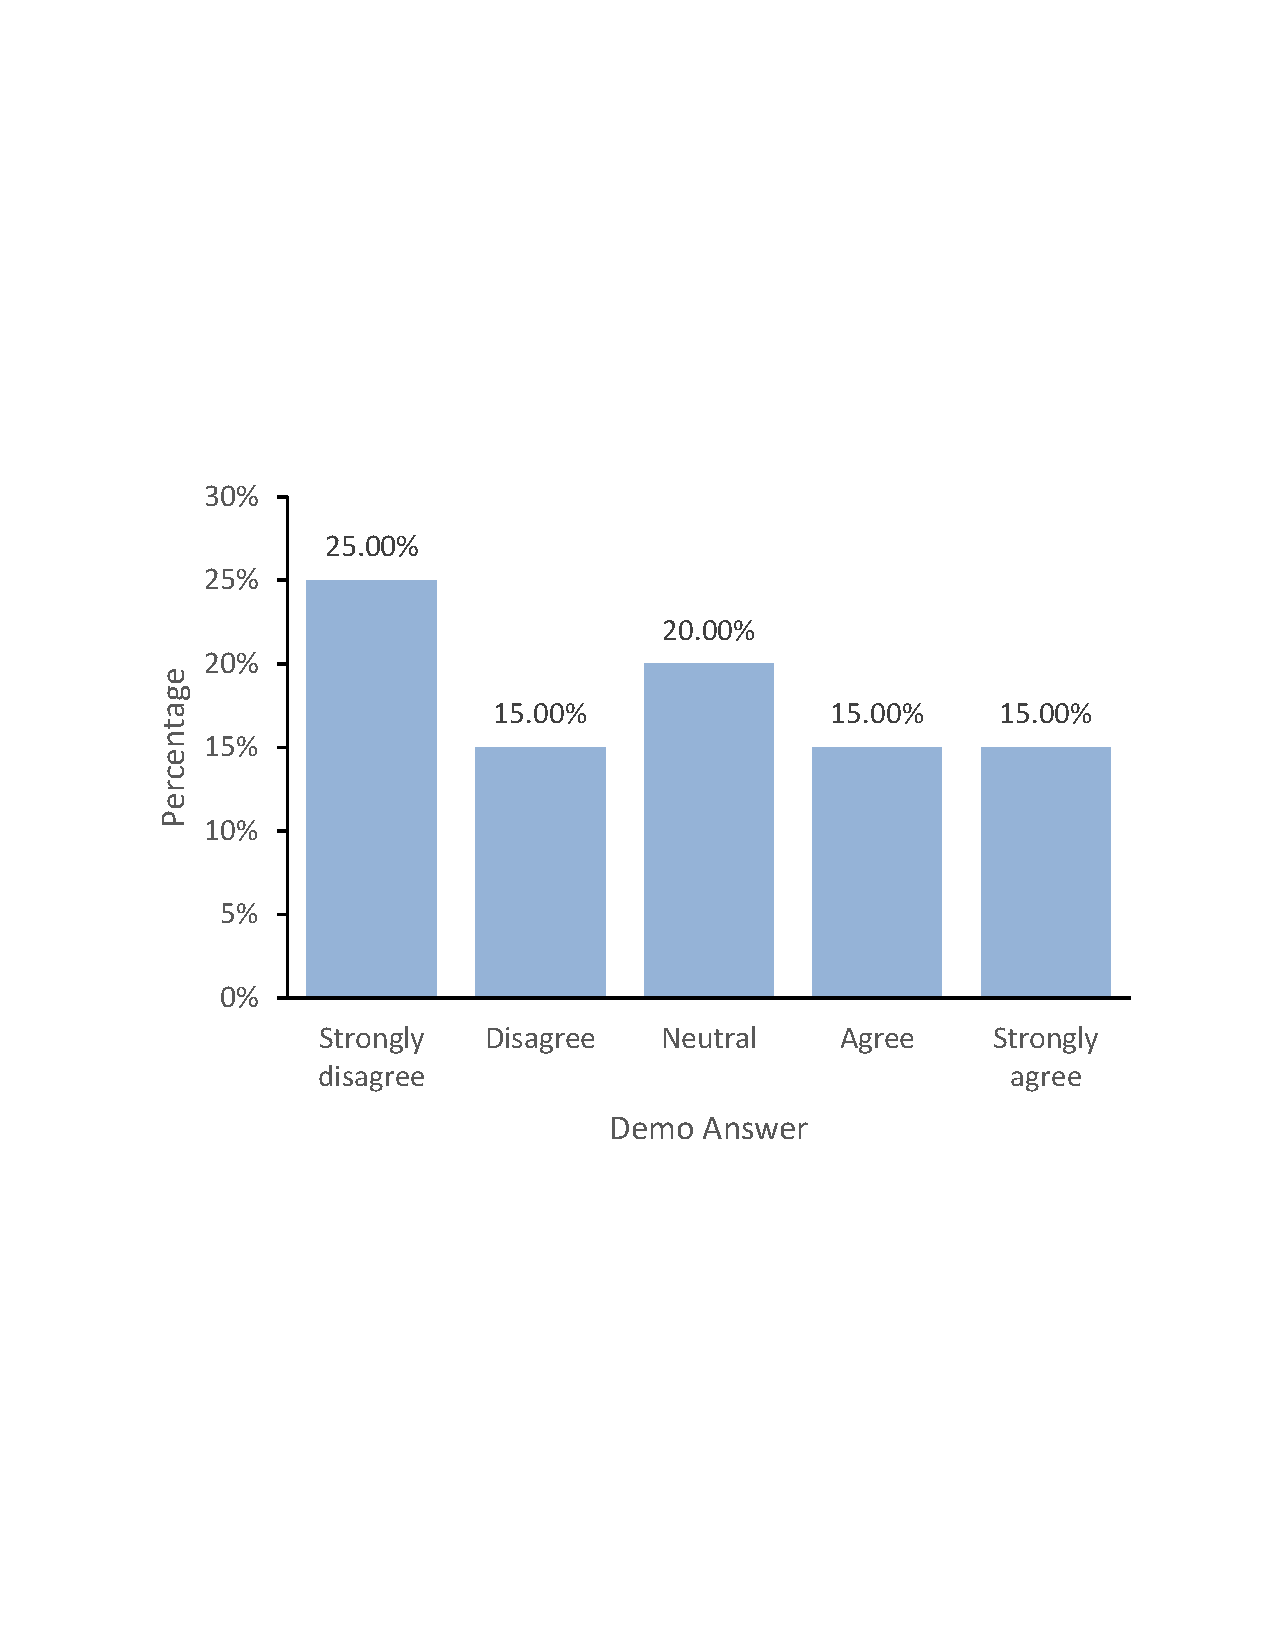
\includegraphics[width=.45\linewidth]{study/complex.pdf}}\hfill
\subfloat[The evaluation result of - "I think that I would need a tutorial before using this visualization tool"\label{fig:introTutorial}]
  {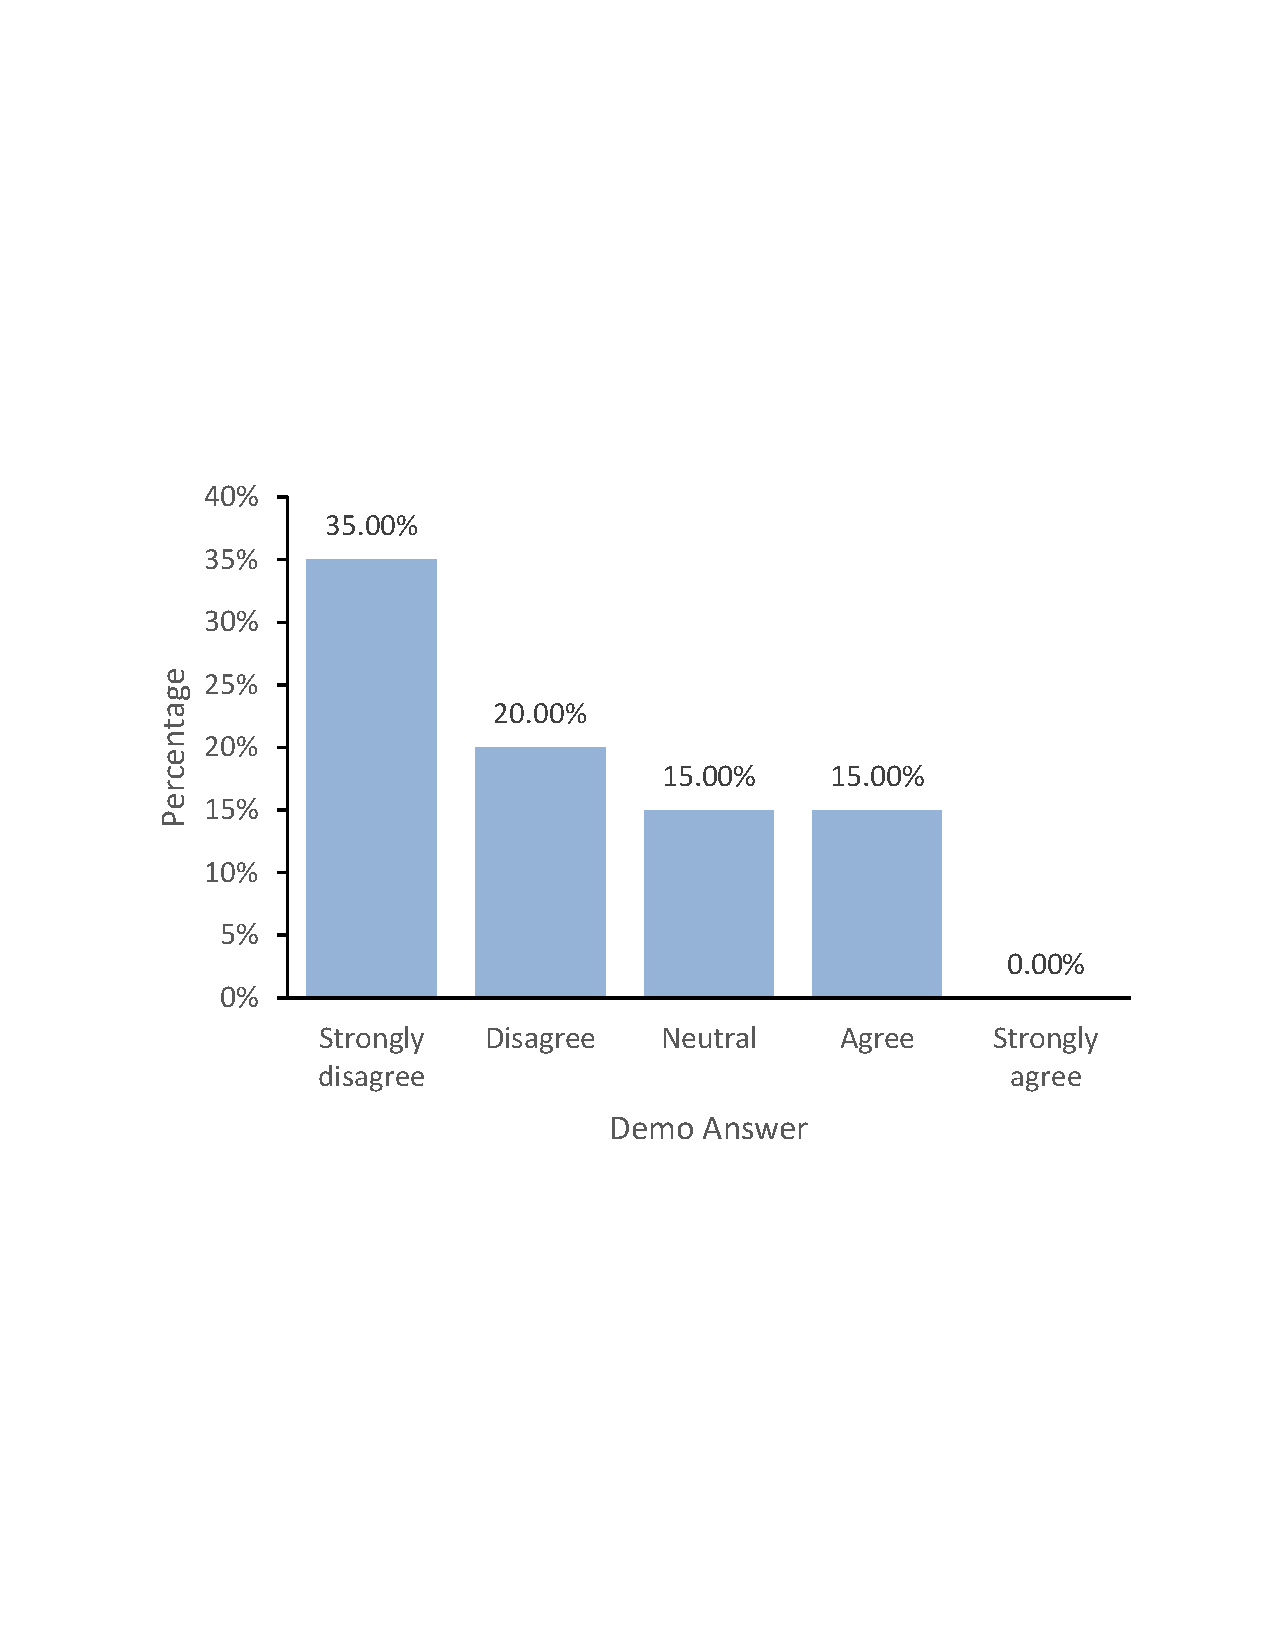
\includegraphics[width=.45\linewidth]{study/intro.pdf}}
\hfill
\caption{The evaluation result of complete visualization tool}
\label{fig:selfExp}
\end{center}
\end{figure}

In figure \ref{fig:finalRev}, the evaluation results are shown ordered by participants based on the map usability and its usefulness. 22 participants completed this question group. Total usability test got a score of 73 where 60\% of the participants rated above than average score and they think the map is very informative and its interactivity is not really complex. 40\% of the participants found it difficult to use and rated less than the average score.

\begin{figure} 
  \begin{center}
    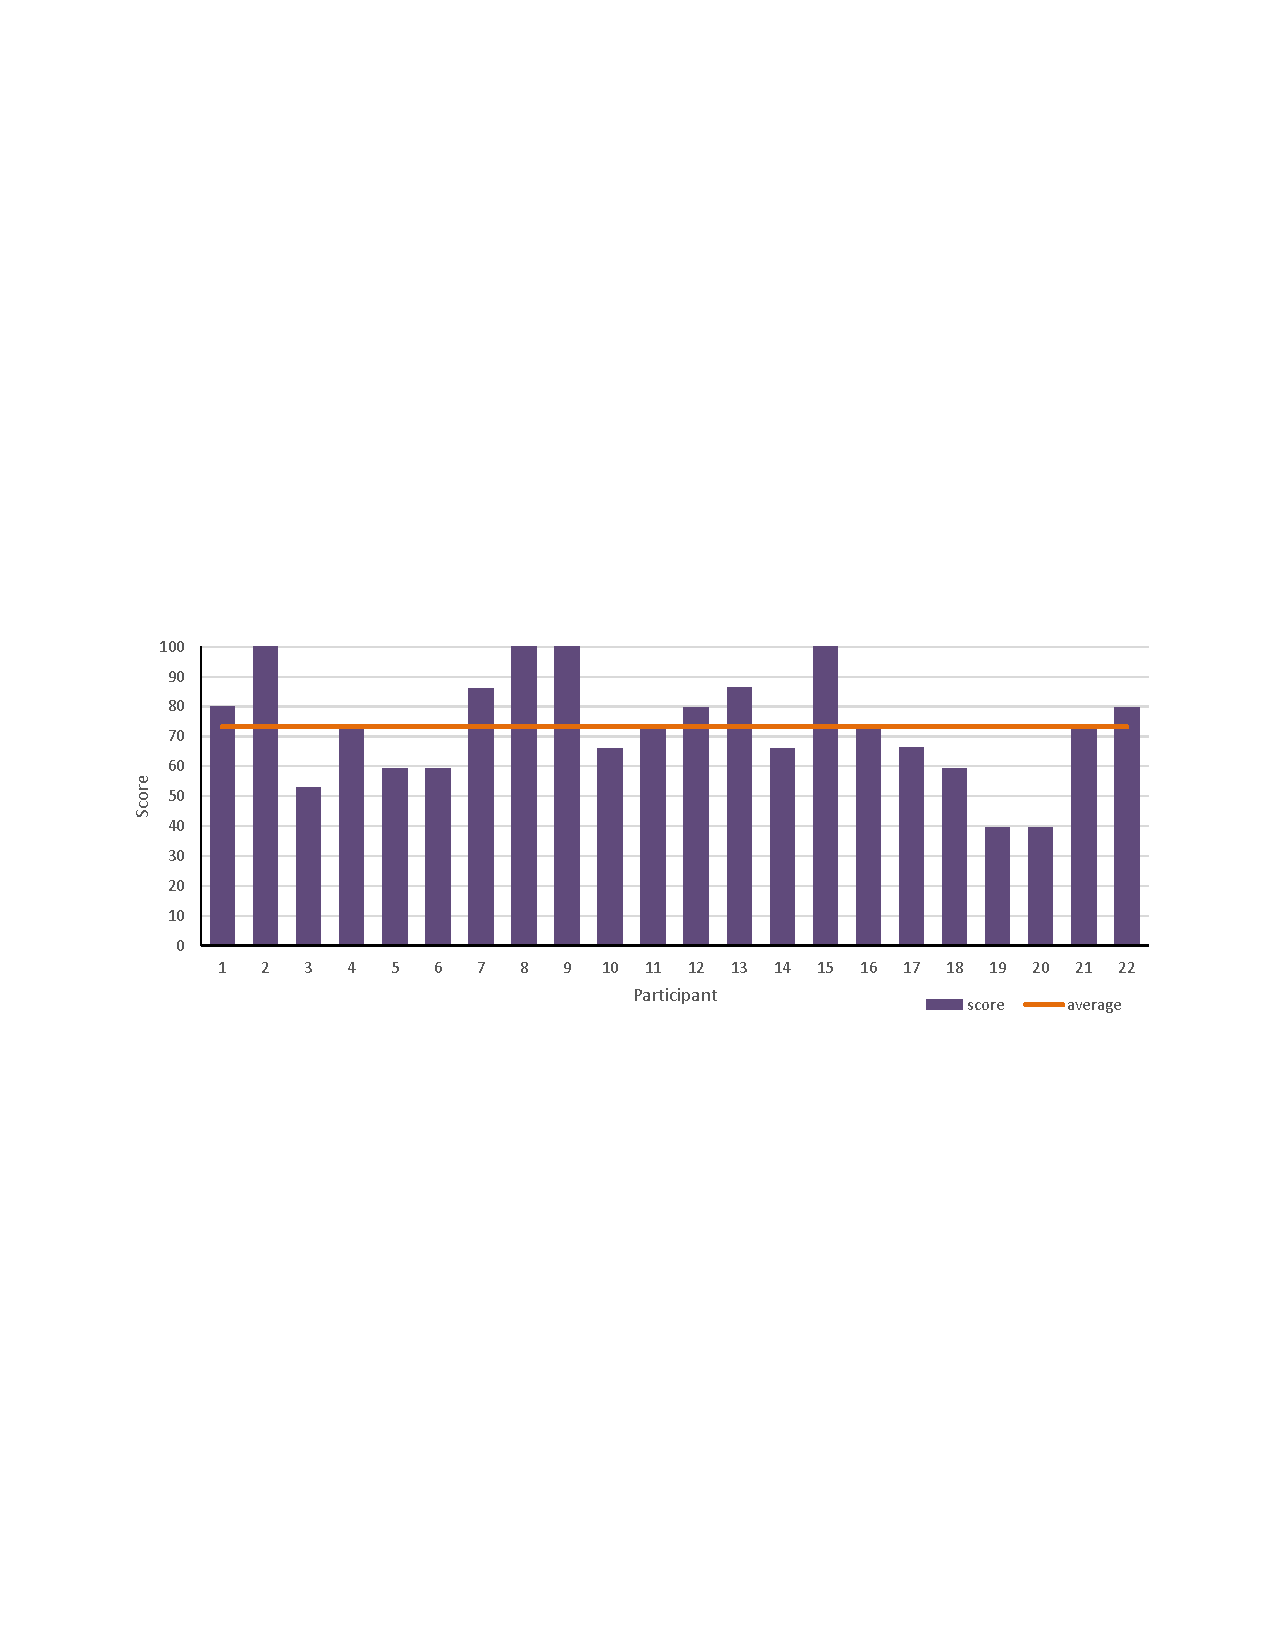
\includegraphics[width=1\textwidth]{study/finalreview.pdf}
    \caption{The result of online survey - complete map usability and usefulness}
    \label{fig:finalRev}
  \end{center}
\end{figure}

\section{User Feedback}

Besides having this information about the power plants the participants in general desired more information from the system. Because of missing information on solar power plants, they proposed to include solar in the information list. Participants also requested to include the city where the plant is located in the marker pop-up. Participants got confused when they saw the marker cluster layer and proposed to omit this feature. The participants also mentioned about difficulties for finding some features, for example, comparison table. Participants also talked about the limitation of comparison table and energy charts. They are interested to compare power plant units from different energy sources on energy chats. They are also interested to see power plants production in bar charts. Participants also requested to have this map in German language. People from social media also shared their thoughts and ideas who didn't participate in the survey. Their thoughts were quite similar with the survey participants. A user said, \textit{“No information on solar!”}. Another social media use provided some important information regarding the correctness of geographical location of power plants.   Another user commented on the 220kV and 380kV power lines and their information. Information provided for the power lines in the map are outdated. However, users from social media noticed the work, got fascinated by the tool and appreciated saying, \textit{“Great Stuff”, "The Map is very informative"}.  

\section{Summary}

The online interactive map was evaluated using an online survey for one week. In this very short time we received 23 survey reports . The study was focused on the qualitative feedback of the map user who are renewable energy professionals, professors, students, engineering working in the energy industry, journalist, and teacher. We were able to reach them through this survey and obtained various feedback, thoughts, ideas, suggestion, usability evaluation result as well as appreciations. The qualitative feedback however uncovered some gaps and limitations within the tool which can be included in the list of future work.

\chapter{Discussion}
\label{chap:discussion}

In this chapter the advantages and usefulness of the interactive map as well as the user-friendliness of this interactive system are highlighted. Furthermore, the weaknesses and difficulties of the system are addressed based on the observation and feedback from the online survey studies. Finally, some complementary approaches to resolve some of these difficulties are outlined.

One of the major advantages of this interactive map is its ability to enable user to get a quick overview of the geographical location of German power plants and high voltage power transmission lines inside Germany.  The interactive map also provides technical data of all power plants and power lines respectively inside the pop-up window and label. The map also provides two more brushing and linking features inside the pop-up window. With “Go to Energy Chart” function, it is possible to see the hourly production of a singular power plant on the energy chart in the form of stacked area chart. “Compare” function generates a comparison table inside the webpage and selected data of that power plants are listed inside the table. Whereas, from the comparison table it is also possible to see the hourly production of the power plant group listed in the table. The navigation menu allows user to select different energy sources and display them on the map in groups. One can select German states to have a closer look and get an idea about the density of power plants and power lines within that specific region. With this new interactive map in combination with energy charts, users can get information on the contribution of renewable and non-renewable energy to power generation in Germany. Survey participants were enthusiastic about having these features in one place. They mentioned that the tool is very informative and easy to use. Although, the map fails to provides some information that user wished for. The data for power plants are periodically collected from European Energy Exchange (EEX) in Leipzig which include power plants which are capable of producing an output of 100MW or more. Our interactive map provides no information on solar power plants and other energy sources with lower generation capacity (less than 100 MW). During the survey, participants were asking for the information on solar and medium sized power plants. Interactive map also shows the high voltage power transmission lines, namely 110 kV, 220 kV and 380 kV. Participants also mentioned their interest in power lines and asked for more technical data about power lines. In the survey, they also mentioned high loading time of power lines on the map. The reason of high loading time was forecasted while developing the interactive map. Large GeoJSON file causes high loading time and for this purpose irresponsiveness is visible on the map. A dedicated database could solve this problem. Map API provides a fully clickable interactive system for the user. Therefore, many users found it user-friendly. Although, confusion has been raised for novice users while they saw the initial cluster view and didn’t understand how to proceed. They requested to remove this feature and didn’t find it useful. Little experienced users who have been using interactive map or similar application found it easy to use. The participant found the markers, navigation menu, and user interface elements self-explanatory. Nevertheless, the interactivity does not eliminate the need for a tutorial by now. One of the participants could not find the comparison table while taking part in the survey. One approach to solve this problem could be a legend mentioning the map features and its operation on the page. Interactive data drill down and brushing-and-linking function make a strong connection with energy charts where user can get up-to-date data on German electricity production. 

The interactive map of energy chats is consistently expanding therefore the view of the map UI and its functionality might be changed over time. At the same time, the operation and other requested additional features by participants will be considered for increasing its usability from novice to expert users. The actual goal of the energy chart is to provide a solid data base and make the energy data transparent to the interested users.  


\chapter{Conclusion and Future Work}
\label{chap:conclusion}

The online visualization tool of German power plants is a fully clickable interactive map providing a quick overview of the location of all power plants listed on the European Energy Exchange (EEX) in Leipzig. In addition, the map also illustrates the high voltage power transmission lines (110 kV, 220 kV and 380 kV) running through all Germany. This interactive visualization map has been added to the Energy Charts, driven by the Fraunhofer Institute for Solar Energy System (ISE). Energy charts presents interactive charts on electricity production, electricity stock market prices and import/export of electricity which is very popular and widely used by people from different countries. In the frame of this work, the new interactive application has been developed to extend a new way for accessing electricity production data for each power plant. Glyph based visualization technique is used to design the location marker according to the semantics of the power plants. Every time user clicks on the power plant, a pop-up window appears with technical information about the power plants for example, source category, nominal electricity generation capacity and owner. The visualization tool also offers brushing and linking functionality with energy charts. The map and hourly electricity production chart are interlinked in both ways. The map offers two different ways for establishing this connection with energy charts. Firstly, map users can see the hourly production of singular power plant or group of power plants on the energy chart. Secondly with the function “Compare”, the selected power plants are listed in a table for comparison and at the end user can see their production on energy charts. Interactive map source selection includes hydro, biomass, nuclear, brown coal (lignite), hard coal, oil, gas, pumped storage, seasonal storage, wind, and garbage power plants. One can either see the power plants in groups or select the plants according to their groups. No data on solar power plant are available in this information visualization, since the EEX list contains only those plants that are larger than 100 MW. There are no solar plant exists in Germany with such a large capacity.  However, energy chart provides hourly electricity production of hydro, nuclear, lignite, hard coal, gas, oil, pumped storage, and wind power plants units. Furthermore, energy chart is also connected with the interactive map. User can see the location of all power plants on the map if a source category is selected on the energy charts. Therefore, both map and energy charts are interlinked with each other. 

The online survey evaluation study showed that the participants adapted the tool very well and very positive about the new application. Furthermore, participants found the tool very informative and using this tool for getting everyday which is noticed from the online access pattern of the user all over the world.  

\section*{Future Work}




%
%
%\renewcommand{\appendixtocname}{Anhang}
%\renewcommand{\appendixname}{Anhang}
%\renewcommand{\appendixpagename}{Anhang}
\backmatter
\appendix
\chapter{Appendix}

\includepdf[scale=0.8,pages={31-38}]{graphics/appendix/Survey_Report.pdf}



%\printindex
%\bibliographystyle{alphadin}
\ifdeutsch
\bibliographystyle{bibliography/IAASde} %f"ur deutsche Texte
\else
\bibliographystyle{bibliography/IAAS} %f"ur englische Texte
\fi
\bibliography{bibliography/mendeley/library}
\ifdeutsch
Alle URLs wurden zuletzt am 17.\,03.\,2008 geprüft.
\else
All links were last followed on \today.
\fi

\backmatter 
\pagestyle{empty}
\renewcommand*{\chapterpagestyle}{empty}
\Versicherung
\end{document}
